% Tipe dokumen adalah report dengan satu kolom. 
% Menggatur setting halaman 
\documentclass[12pt, a4paper, onecolumn, oneside, final]{report}
\makeatother
\usepackage{amsmath}
\usepackage{float}
\usepackage{array}
\usepackage{longtable}
\usepackage{adjustbox}
% Load konfigurasi LaTeX untuk tipe laporan thesis
\usepackage{if_ithb}
\usepackage{enumitem}
\usepackage{multirow}
% Daftar pemenggalan suku kata dan istilah dalam LaTeX
%
% Hyphenation untuk Indonesia 
%
% @author  Enggar Alfianto
% @version 1.00
% 
% Tambahkan cara pemenggalan kata-kata yang salah dipenggal secara otomatis 
% oleh LaTeX. Jika kata tersebut dapat dipenggal dengan benar, maka tidak 
% perlu ditambahkan dalam berkas ini. Tanda pemenggalan kata menggunakan 
% tanda '-'; contoh:
% menarik
%   --> pemenggalan: me-na-rik
%

\hyphenation{
    % alphabhet A
    a-na-li-sa a-tur 
    a-pli-ka-si 
    a-na-li-tik
    % alphabhet B
    ba-ngun-an 
    be-be-ra-pa 
    ber-ge-rak
    ber-ke-lan-jut-an 
    ber-pe-nga-ruh
    bim-bing-an 
    % alphabhet C
    ca-ri
    % alphabhet D
    di-sim-pan di-pim-pin de-ngan da-e-rah di-ba-ngun da-pat di-nya-ta-kan 
    di-sim-bol-kan di-pi-lih di-li-hat de-fi-ni-si
    di-rahmat-i
    di-identifi-kasi-kan
    di-re-pre-sen-ta-si-kan
    du-kung-an-nya
    % alphabhet E
    e-ner-gi eks-klu-sif
    % alphabhet F
    fa-si-li-tas
    fe-no-me-na
    % alphabhet G
    ga-bung-an ge-rak
    % alphabhet H
    ha-lang-an
    hamilton-nia-nya
    % alphabhet I
    % alphabhet J
    % alphabhet K
    ke-rapat-an
    ke-hi-lang-an
    ku-ning 
    kompu-tasi
    kua-li-tas ka-me-ra ke-mung-kin-an ke-se-pa-ham-an
    % alphabhet L
    ling-kung-an
    % alphabhet M
    me-nge-luar-kan
    me-neng-ah
    mem-perhitung-kan
    mem-ban-ding-kan
    meng-a-tas-i me-mung-kin-kan me-nge-na-i me-ngi-rim-kan 
    meng-u-bah meng-a-dap-ta-si me-nya-ta-kan mo-di-fi-ka-si
    meng-a-tur
    % alphabhet N
    nya-ta non-eks-klu-sif
    nano-tekno-logi
    % alphabhet O
    % alphabhet P
    pa-ling
	pe-nye-rap-an 
	pe-ngon-trol
    pe-mo-del-an
    pe-ran  pe-ran-an-nya
    pem-ba-ngun-an pre-si-den pe-me-rin-tah prio-ri-tas peng-am-bil-an 
    peng-ga-bung-an pe-nga-was-an pe-ngem-bang-an 
    pe-nga-ruh pa-ra-lel-is-me per-hi-tung-an per-ma-sa-lah-an 
    pen-ca-ri-an peng-struk-tur-an
    % alphabhet Q
    % alphabhet R
    ran-cang-an
    % alphabhet S
    si-mu-la-si sa-ngat
    se-bagai
    semi-konduktor
    % alphabhet T
    te-ngah
    ter-da-pat
    ter-selesai-kanya 
    % alphabhet U
    % alphabhet V
    % alphabhet W
    % alphabhet X
    % alphabhet Y
    % alphabhet Z
    % special
}

% Variabel baru untuk menyimpan nomor halaman
\newcounter{originalpagenumber}%

% Awal bagian penulisan laporan
\begin{document}

	% Sampul Laporan
	\begin{titlepage}
\begin{center}
	\onehalfspacing
	{\large \bfseries PENERAPAN SUPPORT VECTOR MACHINE UNTUK DETEKSI SARKASME PADA ANALISIS SENTIMEN MEDIA SOSIAL INDONESIA\\
	\vspace{1.5cm}
	 \large TUGAS AKHIR}\\
           Diajukan sebagai syarat untuk menyelesaikan\\ Program Studi Strata-1 Departemen Informatika

	\vspace{1.5cm}
          {\bfseries Disusun Oleh: \\
           Candra Ricky Susanto \\
	1114046}
	
	\vspace{1.5cm}
	
\includegraphics[width=8cm]{images/ithb.jpg}
	
	
	\vspace{3.5cm}
	
{\large \bfseries DEPARTEMEN INFORMATIKA \\
INSTITUT TEKNOLOGI HARAPAN BANGSA \\
BANDUNG\\
2017}

	
\end{center}

\end{titlepage}

\newpage
	
	% Daftar isi, gambar, dan tabel
	% Gunakan penomeran Romawi (i, ii, iii, ...) setelah bagian ini.

	\newcounter{savepage}
	\pagenumbering{roman}
	
	% Lembar Pengesahan
	\phantomsection \addcontentsline{toc}{chapter}{LEMBAR PENGESAHAN}
	\renewcommand{\headrulewidth}{3pt} 
\lhead{
\includegraphics[width=0.3\textwidth]{images/ithb.jpg}\\[0.01cm]}
\rhead{{\bfseries DEPARTEMEN INFORMATIKA \\
 INSTITUT TEKNOLOGI HARAPAN BANGSA\\[0.01cm]}}
\thispagestyle{fancy}

\hspace{-2cm}\\[1cm]
\begin{center}
{\bfseries LEMBAR PENGESAHAN}\\[1.0 cm]
{\bfseries PENERAPAN DAN PERBANDINGAN ARSITEKTUR MICROSERVICE TERHADAP ARSITEKTUR MONOLITIK UNTUK KASUS RAWAT JALAN PADA PERANGKAT LUNAK SISTEM INFORMASI MANAJEMEN RUMAH SAKIT} \\[0.5 cm]
\end{center}

\vspace{0.5cm}
%\begin{wrapfigure}{r}{0.90\textwidth}
%
\includegraphics[width= 3.5 cm, height= 5 cm]{images/icon.jpg}
%\vspace{-5cm}
%\vspace{1cm}
%\end{wrapfigure} 

%\hspace{1.5cm}
%\begin{table}[ht]
%\centering
%\hspace{-1.3cm} Disusun Oleh:\\
%	\begin{tabular}{lll}
%		\hspace{2 cm} Nama & : & XXX XXX XXX\\
%		\hspace{2 cm} NIM & : & XXXXXXX \\
%	\end{tabular}
%\end{table} 
%\\[1.5cm]

\begin{center}   
\begin{tabular}{ p{4.5cm}  p{5.5cm}}
 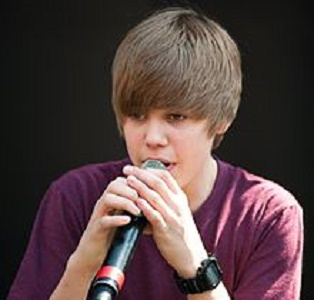
\includegraphics[width=4cm, height =6cm]{images/bieber.jpg} &
\vspace{-4cm}{Disusun oleh:\newline Nama: Edric Laksa Putra\newline NIM	: 1114065}

\end{tabular}
\end{center}
\doublespacing
{\center
\vspace{1cm}
Telah Disetujui dan Disahkan\\ Sebagai laporan Tugas Akhir Departemen Informatika\\
Institut Teknologi Harapan Bangsa\\[0.5cm]
Bandung,   Desember 2017\\
Disetujui,\\[0.5cm]
Pembimbing\\[2cm]
\bfseries 
{\underline {Irfin Afifudin, S.T., M.T.}\\
NIK. \\}}

	% Lembar Pernyataan Pribadi
	\phantomsection \addcontentsline{toc}{chapter}{LEMBAR PERNYATAAN HASIL KARYA PRIBADI}
	\renewcommand{\headrulewidth}{3pt} 
\lhead{
\includegraphics[width=0.3\textwidth]{images/ithb.jpg}\\[0.01cm]}
\rhead{{\bfseries DEPARTEMEN INFORMATIKA \\
 INSTITUT TEKNOLOGI HARAPAN BANGSA\\[0.01cm]}}
\thispagestyle{fancy}

\hspace{-2cm}\\[1cm]
\begin{center}
{\bfseries PERNYATAAN HASIL KARYA PRIBADI}\\[1.0 cm]
\end{center}
Saya yang bertanda tangan di bawah ini:\\[0.5 cm]
\renewcommand{\arraystretch}{1.5}
\begin{table}[ht]
	\begin{tabular}{lll}
		Nama & : & Candra Ricky Susanto \\
		NIM & : &  1114046\\
	\end{tabular}
\end{table} 
\\Dengan ini menyatakan bahwa laporan Tugas Akhir dengan Judul : ” {\bfseries PENERAPAN SUPPORT VECTOR MACHINE UNTUK DETEKSI SARKASME PADA ANALISIS SENTIMEN MEDIA SOSIAL INDONESIA}” adalah hasil pekerjaan saya dan seluruh ide, pendapat atau materi dari sumber lain telah dikutip dengan cara penulisan referensi yang sesuai.\\[0.5 cm]
Pernyataan ini saya buat dengan sebenar-benarnya dan jika pernyataan ini tidak sesuai dengan kenyataan maka saya bersedia menanggung sanksi yang akan dikenakan pada saya.

\noindent
\vspace{0.3cm}
\begin{tabularx}{\linewidth}{XX}

\begin{minipage}{\linewidth}\raggedleft
\vspace{2cm}
Bandung, Desember 2017\\
Yang membuat pernyataan,\\
\vspace{2cm}
Candra Ricky Susanto\\
\end{minipage}
\end{tabularx}

	% Lembar Abstrak
	\phantomsection \addcontentsline{toc}{chapter}{ABSTRAK}
	\chapter*{ABSTRAK}

\noindent Arsitektur perangkat lunak merupakan ringkasan yang menguraikan organisasi standar proses perangkat lunak. Arsitektur ini menguraikan pemesanan, antarmuka, kesalingbergantungan, dan hubungan lainnya di antara unsur-unsur organisasi standar proses perangkat lunak \cite{14}. Tantangan pada analisis penelitian adalah mengembangkan arsitektur \textit{microservice} untuk mengatasi masalah pada arsitektur \textit{monolithic} pada sistem yang semakin besar untuk menjaga sinergi dari sistem tetap efisien \cite{9}. Contoh kasus yang diangkat untuk penelitian ini adalah sistem rawat jalan pada Sistem Informasi Manajemen Rumah Sakit Apertura. Pengembangan arsitektur \textit{microservice} diawali dengan menentukan modul \textit{service} yang terbentuk dari hasil dekomposisi proses bisnis \cite{6}, dengan menggunakan \textit{pattern database per service} \cite{6}. Metode komunikasi antar \textit{service} menggunakan RESTful (\textit{Representational State Transfer}) API dengan format data yang dikirimkan berupa JSON (\textit{JavaScript Object Notation}) \cite{9} dan metode \textit{API Composition} untuk melakukan \textit{in-memory join} \cite{6}. Pengujian dilakukan dengan melakukan perbandingan analisa dari cara sistem bekerja untuk setiap parameter uji yang terdiri dari : tingkat performa, availabilitas, skalabilitas, dan reliabilitas sistem \cite{10}. Berdasarkan hasil analisa pengujian, arsitektur \textit{microservice} dapat menjadi solusi dalam menyelesaikan kendala dalam arsitektur \textit{monolithic} dan cocok diterapkan pada sistem Apertura untuk pengembangan sistem beberapa tahun kedepan.

\noindent\textbf{Kata Kunci}: \textit{Monolithic}, \textit{Microservice}, Arsitektur Perangkat Lunak, Rekayasa Perangkat Lunak.

	% Lembar Abstract
	\phantomsection \addcontentsline{toc}{chapter}{ABSTRACT}
	\chapter*{ABSTRACT}
\noindent The software architecture is a summary that describes the organization standard software process. This architecture outlines reservations, interfaces, interdependencies, and other relationships among the elements the standard organization of software processes [14]. Challenges on research analysis is developing microservice architecture to solve the problem on monolithic architecture on an increasingly large system to keep synergies from the system remains efficient [9]. Examples of cases raised for this study are outpatient system at Apertura Hospital Management Information System. Development of microservice architecture begins with determining the service module which is formed from the decomposition of business processes [6], using database per service pattern [6]. Communication methods between services use RESTful (Representational State Transfer) API with a data format delivered in the form of JSON (JavaScript Object Notation) [9] and API methods Composition to perform in-memory join [6]. Testing done with perform comparison comparisons of the way the system works for each parameter test consisting of: level of performance, availability, scalability, and reliability system [10]. Based on the result of testing analysis, microservice architecture can be the solution in solving constraints in monolithic and architecture suitable applied to Apertura system for multiple system development years ahead.

\noindent\textbf{Keyword}: Monolithic, Microservice, \textit{Arsitektur Perangkat Lunak}, \textit{Rekayasa Perangkat Lunak}.

	% Lembar Pedoman
	\phantomsection \addcontentsline{toc}{chapter}{PEDOMAN PENGGUNAAN TUGAS AKHIR}
	
%
% Halaman Pedoman Pengunaan Tugas Akhir

\chapter*{PEDOMAN PENGGUNAAN TUGAS AKHIR}
{\raggedleft Laporan tugas akhir yang tidak dipublikasikan terdaftar dan tersedia di Perpustakaan Institut Teknologi Harapan Bangsa, dan terbuka untuk umum dengan ketentuan bahwa hak cipta ada pada pengarang dan pembimbing Tugas Akhir. Referensi kepustakaan diperkenankan dicatat, tetapi pengutipan atau peringkasan hanya dapat dilakukan dengan seizin pengarang atau pembimbing Tugas Akhir dan harus disertai dengan ketentuan penulisan ilmiah untuk menyebutkan sumbernya.}\\[1.0 cm]
Tidak diperkenankan untuk memperbanyak atau menerbitkan sebagian atau seluruh laporan tugas akhir tanpa seizin dari pengarang atau pembimbing Tugas Akhir yang bersangkutan.


\newpage


	% Kata Pengantar
	\phantomsection \addcontentsline{toc}{chapter}{KATA PENGANTAR}
	% Kata Pengantar
\chapter*{KATA PENGANTAR}
{\raggedleft Terima kasih kepada Tuhan yang Maha Esa karena dengan bimbingan-Nya dan karunia-Nya penulis dapat melaksanakan Tugas Akhir yang berjudul \textquotedblright PENERAPAN METODE LABELED LATENT DIRICHLET ALLOCATION DENGAN TF-IDF UNTUK KATEGORISASI DOKUMEN\textquotedblleft. Laporan ini disusun sebagai salah satu syarat kelulusan di Institut Teknologi Harapan Bangsa. Pada kesempatan ini penulis menyampaikan terima kasih yang sebesar-besarnya kepada:} \\
\begin{enumerate}
\item Tuhan Yang Maha Esa, karena oleh bimbingan-Nya penulis selalu mendapat pengharapan untuk menyelesaikan tugas akhir ini.
\item Ibu Ria Chaniago, S.T., M.T., selaku pembimbing I Tugas Akhir yang  senantiasa memberi dukungan, semangat, ilmu-ilmu, saran dan dukungan kepada penulis selama tugas akhir berlangsung dan selama pembuatan laporan tugas akhir ini.
\item Bapak Firhat Hidayat, S.T., M.T., selaku penguji I Tugas Akhir. Terima kasih atas dukungan, semangat, ilmu-ilmu, dan masukan yang telah diberikan kepada penulis dalam menyelesaikan Laporan Tugas Akhir ini
\item Ibu Ir. Inge Martina, M.T., selaku penguji II dalam Tugas Akhir Terima kasih atas dukungan, semangat, ilmu-ilmu, dan masukan yang telah diberikan kepada penulis dalam menyelesaikan Laporan Tugas Akhir ini.
\item Seluruh dosen dan staff Departemen Teknik Informatika ITHB yang telah membantu dalam menyelesaikan Laporan Tugas Akhir ini.
\item Segenap jajaran staf dan karyawan ITHB yang turut membantu kelancaran dalam menyelesaikan Laporan Tugas Akhir ini.
\item Kedua orang tua tercinta yang selalu menyediakan waktu untuk memberikan doa, semangat dan dukungan yang tak habis-habisnya kepada penulis untuk menyelesaikan Laporan Tugas Akhir ini. Terima kasih untuk nasihat, masukan, perhatian, teguran dan kasih sayang yang diberikan hingga saat ini.
\\
\end{enumerate}
Penulis menyadari bahwa laporan ini masih jauh dari sempurna karena keterbatasan waktu dan pengetahuan yang dimiliki oleh penulis. Oleh karena itu, kritik dan saran untuk membangun kesempurnaan tugas akhir ini sangat diharapkan. Semoga tugas akhir ini dapat membantu pihak-pihak yang membutuhkannya.\\[1.5cm]  
\hfill
{\begin{flushright} Bandung, Desemeber 2017\\[1.5cm] Hormat  Saya,\\ Devit Lie.\end{flushright}}
\newpage
	
	\vspace*{-2.5cm}
	\tableofcontents
	\phantomsection
	\addcontentsline{toc}{chapter}{DAFTAR ISI}
	\clearpage
	\vspace*{-2.5cm}
	\listoftables
	\phantomsection
	\addcontentsline{toc}{chapter}{DAFTAR TABEL}
	\clearpage
	\vspace*{-2.5cm}
	\listoffigures
	\phantomsection
	\addcontentsline{toc}{chapter}{DAFTAR GAMBAR}
	\clearpage
	
	\setcounter{savepage}{\arabic{page}}
	\makeatletter
	\def\MyPagenumbering#1{%
		\global\c@page \@ne \gdef\thepage{\arabic{chapter}-\csname @#1\endcsname
			\c@page}}
	\makeatother
	\pagestyle{fancy}
	\renewcommand{\chaptermark}[1]{%
		\markboth{\thechapter.\ #1}{}}
	
	\fancyhf{}
	% Gunakan penomeran Arab (1, 2, 3, ...) setelah bagian ini.
	\MyPagenumbering{arabic}
	
	% Untuk mengatur posisi pagenumber
	%\pagestyle{plain}
	\setlength\LTleft{0pt}            % default: \fill
	\setlength\LTright{0pt}           % default: \fill
	\lhead{\leftmark}
	\renewcommand{\headrulewidth}{1pt}
	
	\fancypagestyle{plain}{%
		\renewcommand{\headrulewidth}{0pt}%
		\fancyhf{}%
		\fancyfoot[R]{\arabic{chapter}-1}%
	}
	
	\onehalfspacing
	\setcounter{page}{1}
	\rfoot{\arabic{chapter}-\arabic{page}}
	%-----------------------------------------------------------------------------%
\chapter{PENDAHULUAN}
%-----------------------------------------------------------------------------%

\vspace{4.5pt}

\section{Latar Belakang Masalah} \label{sec:latar_belakang}
Sistem komputer adalah interaksi dari perangkat lunak dan perangkat keras yang membentuk sebuah jaringan elektronik. Tugas dari sebuah sistem adalah menerima input, memproses data input, menyimpan data olahan, dan menampilkan output sebagai bentuk informasi. Dalam penerapannya, kita menyebut sistem aplikasi sebagai program komputer yang bertugas untuk menyelesaikan kebutuhan khusus. Terdapat beberapa tahapan umum dalam mengembangkan sistem aplikasi yaitu perencanaan, analisa, desain, pengembangan, testing, implementasi, dan pemeliharaan [1].  Tahap yang cukup penting dan akan menjadi fokus diskusi adalah desain dan pengembangan, yang dimana peran arsitektur perangkat lunak sangat berperan penting untuk menetapkan landasan dasar pengembangan aplikasi dari awal sampai selesai. Hasil dari arsitektur perangkat lunak merupakan struktur yang melandasi keberadaan komponen-komponen perangkat lunak, cara komponen untuk saling berinteraksi dan organisasi komponen dalam membentuk perangkat lunak [2]. Arsitektur yang paling sering digunakan saat ini adalah model monolitik. Arsitektur monolitik merupakan arsitektur yang mudah dimengerti dan dimodifikasi karena lebih sederhana implementasinya. Arsitektur ini menggunakan kode sumber dan teknologi yang serupa untuk menjalankan semua tugas-tugasnya. Secara garis besar keunggulan dari arsitektur monolitik dapat dirasakan apabila aplikasi ingin mudah untuk dikembangkan, mudah untuk di deploy, dan dapat selalu dipantau pertumbuhan perfomanya [5]. Namun apabila aplikasi semakin besar dan anggota tim semakin banyak, arsitektur monolitik akan menghadapi kekurangan yang semakin lama akan semakin signifikan. Kelemahan dari arsitektur monolitik dapat dirasakan dari sisi \textit{deployment}, tingkat keamanan, tingkat ketersediaan, dan manajemen aplikasi yang semakin sulit dan kualitasnya menurun \cite{8}.\\
Pada tahun 2015 sebuah arsitektur microservice merupakan arsitektur alternatif yang dapat mengatasi kelemahan dari monolitik. Arsitektur microservice menjadikan sebuah aplikasi lebih mandiri dan efisien. Namun kendala yang sering menjadi hambatan adalah setiap kasus memiliki masalah dan desain yang berbeda satu dengan yang lain, sehingga dibutuhkan desain microservice yang tepat untuk setiap kasus yang diangkat. Kendala lain adalah sulitnya implementasi arsitektur baru, dibutuhkan panduan yang menjelaskan tahap migrasi dari arsitektur monolitik hingga menjadi microservice. Pada tahap terakhir, uji perbandingan dibutuhkan untuk menjadi parameter keberhasilan arsitektur yang baru.\\
Penelitian ini akan mengangkat contoh kasus penerapan arsitektur microservice pada sistem informasi manajemen rumah sakit Apertura. Penelitian ini bertujuan untuk membuktikan bahwa arsitektur microservice dapat memberikan performa yang lebih baik untuk aplikasi Apertura di kemudian hari.
\section{Rumusan Masalah}
Berikut ini adalah rumusan masalah yang dibuat berdasarkan latar belakang di atas:
\begin {enumerate}[nolistsep, leftmargin=0.5cm]
\item Bagaimana melakukan migrasi dari arsitektur monolitik ke model arsitektur microservice?
\item Bagaimana perbandingan performa yang dihasilkan dari arsitektur microservice yang baru terhadap arsitektur monolitik?
\end{enumerate}

\section{Batasan Masalah}
Batasan masalah pada penelitian ini adalah penelitian hanya berfokus pada perancangan \textit{service} pada arsitektur microservice serta penerapannya secara general untuk ditinjau peluang dan keunggulannya dibandingkan arsitektur monolitik.

\section{Tujuan Penelitian}
Berdasarkan batasan masalah di atas, berikut ini adalah tujuan penelitian dari tugas akhir ini:
\begin{enumerate}[nolistsep,leftmargin=0.5cm]
\item Menentukan bagaimana tahap yang benar untuk melakukan migrasi dari arsitektur monolitik ke arsitektur microservice.
\item Membandingkan apa saja kelebihan dan kekurangan dari arsitektur microservice dibandingkan dengan arsitektur monolitik.
\end{enumerate}

\section{Kontribusi Penelitian}
Berikut ini adalah kontribusi penelitian yang diberikan pada pengembangan sistem analisis sentimen ini:
\begin{enumerate}[nolistsep,leftmargin=0.5cm]
\item Memberikan contoh panduan untuk melakukan migrasi dari arsitektur konvensional ke arsitektur microservice pada sistem informasi manajemen rumah sakit.
\item Memberikan hasil perbandingan arsitektur microservice dan monolitik.
\end{enumerate}

\section{Metode Penelitian}
Tahapan-tahapan yang akan dilakukan dalam pelaksanaan penelitian ini adalah sebagai berikut:
\begin{enumerate}[nolistsep,leftmargin=0.5cm]
\item Analisis\\
Melakukan studi literatur dan analisa melalui wawancara dengan pihak perancang aplikasi monolitik sebelumnya. Data juga dikumpulkan dari jurnal-jurnal, karya ilmiah, dan situs yang memberikan informasi yang menunjang mengenai konsep arsitektur microservice dan tahap-tahap implementasi pada aplikasi monolitik.
\item Identifikasi\\
Melakukan identifikasi mengenai target-target yang ingin dicapai setelah menerapkan arsitektur baru. Identifikasi ini berguna untuk menentukan perbandingan apa saja yang akan diperhatikan antara arsitektur microservice dan arsitektur monolitik ketika pengujian dilakukan.
\item Perancangan\\
Perancangan arsitektur microservice meliputi perancangan model dasar (proses bisnis), perancangan sistem basis data, perancangan kelas service yang baru dengan konsep microservice, juga perancangan jalur komunikasi dan pertukaran data antara kelas-kelas service yang akan dibuat.
\item Implementasi\\
Melakukan implementasi hasil perancangan dalam bentuk web service application (server side). Selanjutnya dibuat aplikasi client sederhana untuk input data dan pengujian performa dari arsitektur server yang telah dibuat.
\item Pengujian\\
Melakukan pengujian terhadap rancangan aplikasi microservice yang baru dan aplikasi monolitik dengan menggunakan data rumah sakit untuk mengetahui hasil kinerja dan perbandingan performa antara kedua jenis arsitektur.
\end{enumerate}

\section{Sistematika Penulisan}
Pada penelitian ini peneliti menyusun berdasarkan sistematika penulisan sebagai berikut: \\[0.5cm]
\noindent \textbf{BAB I \hspace{1cm} PENDAHULUAN}
\begin{addmargin}[2.35cm]{0em}
Berisi penjelasan mengenai latar belakang, rumusan masalah, batasan masalah, tujuan penelitian, manfaat penelitian, metodologi penelitian, dan sistematika penulisan laporan penelitian. 
\end{addmargin}
\noindent \textbf{BAB II \hspace{0.8cm} LANDASAN TEORI}
\begin{addmargin}[2.35cm]{0em}
Membahas tentang definisi dari arsitektur microservice, teori-teori pendukung, dan metode penerapan arsitektur baru yang akan dijadikan landasan dan dipelajari serta dirangkum dari berbagai sumber, seperti buku, karya tulis, jurnal, artikel dari situs ilmiah. Juga pembahasan sekilas mengenai arsitektur konvensional yang digunakan sebelumnya.
\end{addmargin}
\noindent \textbf{BAB III \hspace{0.7cm} ANALISIS DAN PERANCANGAN}
\begin{addmargin}[2.35cm]{0em}
Berisi analisa mengenai bagaimana konsep penerapan arsitektur microservice pada aplikasi rumah sakit dan modul-modul apa saja yang akan di migrasi menjadi modul baru untuk diimplementasikan pada tahap selanjutnya. Selanjutnya membahas perancangan aplikasi dari hasil analisa dengan menggunakan arsitektur microservice yang baru.
\end{addmargin}
\noindent \textbf{BAB IV \hspace{0.7cm} IMPLEMENTASI DAN PENGUJIAN}
\begin{addmargin}[2.35cm]{0em}
Berisi implementasi dari hasil perancangan aplikasi dalam bentuk perangkat lunak menggunakan teknologi \textit{web service}. Selanjutnya perangkat lunak diuji fungsi dan performanya dari sisi \textit{client} (pengguna).
\end{addmargin}
\noindent \textbf{BAB V \hspace{0.8cm} KESIMPULAN DAN SARAN}
\begin{addmargin}[2.35cm]{0em}
Memberikan kesimpulan berdasarkan hasil analisis, perancangan, implementasi dan pengujian, serta evaluasi yang dilakukan, juga saran-saran yang dibutuhkan untuk pengembangan lebih lanjut.
\end{addmargin}

\newpage
	\setcounter{page}{1}
	%-----------------------------------------------------------------------------%
\chapter{LANDASAN TEORI}
Pada bab ini akan dijelaskan teori pendukung serta metode yang digunakan untuk mengekstraksi modul-modul yang terdapat pada aplikasi monolitik. Penjelasan teori dimulai dengan pengertian dari arsitektur Microservice, prinsip dan pemodela microservice, membangun arsitktur microservice dari arsitektur monolitik, metode pengembangan aplikasi berbasis Microservice, serta aplikasi rumah sakit Apertura sendiri.
%-----------------------------------------------------------------------------%

%
\vspace{4.5pt}

\section{Arsitektur Microservice}
Arsitektur aplikasi yang memiliki struktur hubungan service yang renggang namun kolaboratif. Tiap service memiliki fungsi yang lebih sempit dan saling berhubungan. Tiap service ini saling berkomunikasi menggunakan web service dan dapat dikembangkan dan di \textit{deploy} secara mandiri. Tiap service memiliki database masing-masing yang saling memisahkan data. 
\subsection{Definisi Arsitektur Microservice}
Aritektur microservice pertama kali muncul untuk memenuhi kebutuhan dan menunjukan bagaimana sebuah aplikasi dapat lebih efektif dalam tahap \textit{production}, juga menunjukan bagaimana cara \textit{development} yang lebih baik dengan memberikan kemampuan kepada mesin untuk saling berkomunikasi. Microservice juga termasuk ke dalam perancangan insfrastrktur mesin sampai skala yang dibutuhkan. Banyak organisasi telah membuktikan dengan berpindah ke arsitektur microservice, aplikasi mereka menjadi lebih cepat dan berani untuk menggunakan teknologi yang baru. Microservice memberikan \textit{developer} kebebasan untuk bereaksi dan mengambil keputusan yang berbeda, memberikan respon yang lebih cepat atas segala kebutuhan dari pengguna aplikasi \cite{9}.
\subsection{Prinsip Pendekatan Arsitektur Microservice}
Terdapat beberapa tahapan dalam pendekatan dalam arsitektur mikroservis yang menjadikan desain system yang baik, pendekatan ini berguna untuk mendefinisikan prinsip dan petunjuk yang bergantung pada gol yang kita tuju, tahapan pendekatan tersebut yaitu :
\begin{enumerate}[leftmargin=*]
	\item \textit{Strategic Goals.} Strategic goals harus memberikan arahan kemana perusahaan ingin beranjak dan bagaimana memenuhi kebutuhan konsumen. Bahasan ini harus berisi tujuan tertinggi dan tidak membahas teknologi sama sekali. Goals ini bisa dibahas di level perusahaan atau juga di level divisi. Kuncinya adalah untuk membuat kemana arah organisasi akan bergerak \cite{9}.
	\item \textit{Principles.} Principles adalah aturan yang harus dibuat agar dapat memenuhi goals, prinsip ini kadang berubah sesuai dengan kondisi. Misalnya apabila strategic goals perusahaan adalah untuk mengurangi waktu pengiriman barang-barang baru, maka organisasi terebut akan mendefinisikan prinsip yang mengatakan bahwa tim pengiriman mempunyai kontrol penuh terhadap \textit{lifecycle} produk mereka untuk dikirimkan kapanpun produk siap. Namun apabila goals adalah untuk mengembangkan pertumbuhan produk dengan cepat di sebuah negara, maka organisasi akan memutuskan untuk mengimplementasi prinsip bahwa semua system harus bisa bekerja secara portable agar dapat di \textit{deploy} secara local dan memastikan bahwa data akurat. Prinsip ini juga jangan terlalu banyak, kurang dari 10 adalah angka yang baik, karena semakin banyak prinsip akan beresiko menjadikan aturan-aturan tersebut saling bentrok satu sama lain \cite{9}.
	\item \textit{Practices.} Tahap ke tiga adalah untuk memastikan semua prinsip telah dilakukan. \textit{Practices} adalah sebuah detail set, bagaimana untuk melakukan task-task agar goals dapat dicapai sesuai dengan aturan yang ada. Tahap ini termasuk dengan spesifikasi teknologi, dan harus cukup sedetail mungkin agar semua \textit{developer} dapat paham. \textit{Practices} dapat termasuk petunjuk bagaimana \textit{lifecycle}coding dilakukan. Sesuai dengan sifat naturalnya, \textit{practices} akan lebih sering berubah dibandingkan dengan principal di tahap ke 2 \cite{9}.
	\item \textit{Combining Principles and Practices.} Ide dari point terakhir ini adalah ketika system berevolusi dengan ide baru, organisasi tetap siap dengan segala detail yang dibutuhkan agar semua orang tahu bagaimana mengimplementasi ide baru tersebut. Terdengar mudah untuk dilakukan di lingkup yang kecil, namun untuk lingkup besar, bisa terdapat perbedaan antara teknologi dengan praktek yang dilakukan. Misalnya tim .NET akan mempunyai set \textit{practices} yang berbeda dengan tim Java \cite{9}.
\end{enumerate}
\subsection{Konsep Microservice}
Setelah pengertian umum mengenai arsitektur microservice, pada bagian ini akan dijelaskan bagaimana cara berfikir dengan batasan-batasan microservice yang akan memaksimalkan semua potensinya. Dalam point ini peneliti menginginkan pembaca fokus terhadap dua konsep kunci microservice, yaitu \textit{loose coupling} dan \textit{high cohesion}.\\
\textbf{\textit{Loose Coupling.}} Ketika service telah \textit{loosely coupled}, perubahan yang dilakukan terhadap satu service tidak akan mengakibatkan perubahan pada service yang lain. Prinsip ini menekankan bagaimana microservice dapat melakukan perubahan pada satu service dan melakukan \textit{deploy} tanpa harus melakukan perubahan apapun pada sistem. Namun sebuah sistem dapat memiliki kebutuhan berkomunikasi antar service, hal ini mengakibatkan arsitek harus membatasi limit panggilan dari satu service terhadap service yang lain, karena selain dapat menyebabkan masalah performa, hal ini pula dapat mengakibatkan terjadinya \textit{tight coupling} \cite{9}.\\
\textbf{\textit{High Cohesion.}} Model microservice menginginkan sifat-sifat yang berkaitan untuk berada di satu wadah, dan yang tidak berkaitan ditempatkan di wadah yang lain, karena apabila ada perubahan yang terjadi, hanya satu wadah tersebut yang akan berubah dan perubahan dapat langsung di implementasikan dengan cepat. Apabila service dibuat terlalu tercecer, maka akan menyebabkan perubahan di banyak tempat dan akan membuang banyak waktu. Point yang diinginkan adalah menempatkan service dengan sifat yang mirip di satu wadah, namun tetap berkomunikasi dengan wadah lain selonggar mungkin \cite{9}.\\
Dalam buku yang dijelaskan Sam Newman, penulis mengambil contoh sebuah departemen keuangan dan departemen \textit{warehouse} di sebuah organisasi untuk menjelaskan tentang shared dan hidden model. Kedua departemen mempunyai \textit{interface} yang berbeda ketika ditampilkan. Departemen keuangan tidak perlu tahu segala detail di \textit{warehouse}. Namun walau begitu tetap ada data yang dibutuhkan seperti misalnya stok barang agar mendapatkan perhitungan terbaru. Pada model microservice maka ke dua modul ini akan dibuat terpisah. Berikut penggambarannya :\\

\begin{adjustbox}{width=1\textwidth}
	\centering
	\begin{minipage}{\linewidth}
		\framebox[\textwidth]{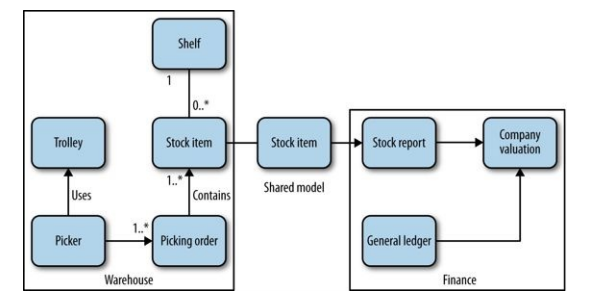
\includegraphics[width=10cm]{images/departements_relation.png}}	
		\captionof{figure}{Model pembagian dari departemen keuangan dan warehouse.}
	\end{minipage}
\end{adjustbox}

Untuk dapat menjalankan alur informasi, pegawai keuangan membutuhkan data stok. \textit{Stock item} menjadi \textit{shared model} antara dua departemen. Perlu diingat bahwa tidak semua data \textit{warehouse} harus diperlihatkan di keuangan, jadi terdapat representasi internal dan representasi external yang diperlihatkan. Desain diatas memperlihatkan konsep \textit{loose coupling} dan \textit{high cohesion} yang digambarkan menjadi sebuah modul. Desain seperti ini sangat mempermudah proses perpindahan dari monolitik dan menyakinkan bahwa desain microservice telah \textit{loosely coupled} dan \textit{stongly cohesive} \cite{9}.
\section{Integrasi Teknologi}
Mengintegrasikan dengan benar merupakan tahap yang paling penting, memungkinkan perubahan yang signifikan dengan tingkat kemandirian aplikasi yang tinggi. Dalam tahap integrasi ini ada beberapa point penting yang harus dianalisis sebelum memilih teknologi yang digunakan dan mengimplementasikannya.
\begin{enumerate}[leftmargin=*]
	\item \textit{\textbf{Menjaga teknologi API agar tetap agnostik.}} IT industri adalah berubah dengan sangat cepat, \textit{tools} baru, \textit{framework} dan bahasa baru, serta ide-ide implementasi yang selalu berkembang. Hal inilah yang menjadi pertimbangan agar memastikan bahwa API inisial harus dapat digunakan terus menerus ketika mengimplementasikan microservice.
	\item \textit{\textbf{Hindari perubahan major pada aplikasi.}} Perubahan arsitektur dapat mengakibatkan perubahan pada bagian-bagian aplikasi yang lainnya, pemilihan teknologi yang tepat bertujuan agar perubahan ini terjadi sekecil mungkin.
	\item \textit{\textbf{Buat service sederhana untuk dipakai.}} Arsitektur microservice yang baru harus cepat beradaptasi dengan penggunanya, maka dari itu modul service harus bersifat \textit{user-friendly}. 
\end{enumerate}
Seperti yang dikutip dari website Chris Richardson, microservice merupakan sekumpulan teknologi yang saling bekerjasama. Teknologi tersebut tidak dibatasi oleh sebuah wadah tertentu, namun saling terpisah yang menyebabkan luasnya pemilihan teknologi yang akan digunakan. Point berikutnya akan menjelaskan beberapa pilihan teknologi yang baik yang dapat diimplementasikan. Mulai dari lapisan paling dalam, yaitu managemen data, pembagian service, metode berkomunikasi antar service, sampai dengan API gateway yang akan digunakan oleh clien \cite{9}.
\subsection{Manajemen Data}
Bab ini akan membahas bagaimana penyimpanan data pada arsitektur monolitik dan apa kelemahannya. Kemudian dilanjutkan dengan penjelasan dan pembahasan metode penyimpanan data yang baik dan sesuai dengan arsitektur microservice.
\subsubsection{Model Penyimpanan Data Arsitektur Monolitik}
Pada arsitektur biasa, umumnya database disimpan dalam 1 tempat dan terdiri dari beberapa table. Ketika terjadi permintaan untuk membaca data, maka sistem akan mengambil data tersebut dari database, sama halnya apabila data diubah, maka sistem akan langsung mengubah database. \textit{Life cycle} seperti ini sangat simpel dan sangat cepat sehingga sampai saat ini dipakai oleh banyak sistem.\\
Contoh dalam gambar 2-1, \textit{customer} yang akan melakukan registrasi akan melakukan \textit{querry} ke database, juga aplikasi \textit{call center} yang menampilkan dan mengubah data akan langsung melakukan \textit{querry} ke database, begitu pula dengan informasi \textit{update warehouse} mengenai pesanan konsumen, akan melakukan \textit{query} pada database. Ini adalah contoh pattern yang sangat umum, namun banyak kelemahan dari pattern database ini \cite{9}

\begin{adjustbox}{width=1\textwidth}
	\centering
	\begin{minipage}{\linewidth}
		\framebox[\textwidth]{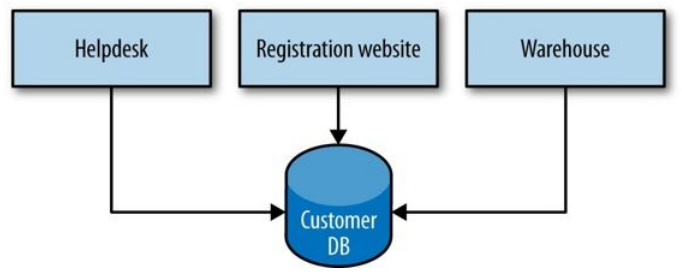
\includegraphics[width=10cm]{images/common_accessing_db.png}}	
		\captionof{figure}{Pemodelan cara akses database yang umum.}
	\end{minipage}
\end{adjustbox}\\

Pertama, model ini mengizinkan langsung pihak luar untuk mengubah data internal. Struktur data yang di simpan di DB dipakai oleh semua \textit{user}, apabila terjadi perubahan pada DB, maka semua \textit{user} akan terkena dampaknya. Database menjadi sangat besar, dan \textit{shared} API menjadi rapuh. Apabila akan terjadi perubahan, misalnya perubahan table customer di database, maka harus sangat berhati-hati agar \textit{schema} yang dipakai oleh service lain tidak rusak. Hal ini membutuhkan usaha testing regresi yang besar. Hal ini melanggar konsep \textit{loose coupling} \cite{9}. Kedua, semua \textit{client} menjadi terikat dengan sebuah teknologi spesifik. Mungkin saat ini database berjalan dengan baik dengan menggunakan \textit{relational} database, namun bagaimana bila seiring berjalannya waktu, performa untuk menyimpan data lebih baik menggunakan \textit{nonrelational} database? \textit{Client} menjadi terikat dengan model implementasi. Hal ini melanggar konsep \textit{cohesion}.
\subsubsection{Model Penyimpanan Data Arsitektur Micoservice}
Dalam perancangan arsitektur microservice, terdapat 2 pattern database ditinjau dari pembagian database tersebut. Pattern pertama adalah \textit{shared database} dan yang kedua adalah \textit{database per service}. Untuk contoh kedua pattern, penulis Chris Richardson memberikan contoh dengan menggunakan modul \textit{customer} dan modul \textit{order}. Hubungan kedua modul tersebut terjadi ketika ada transaksi baru, dimana modul \textit{order} harus memastikan bahwa jumlah pesanan yang baru tidak melebihi limit kredit yang dimiliki \textit{customer}. Relasi kedua modul itu dapat dilihat dari gambar dibawa \cite{6}\\

\begin{adjustbox}{width=1\textwidth}
	\centering
	\begin{minipage}{\linewidth}
		\framebox[\textwidth]{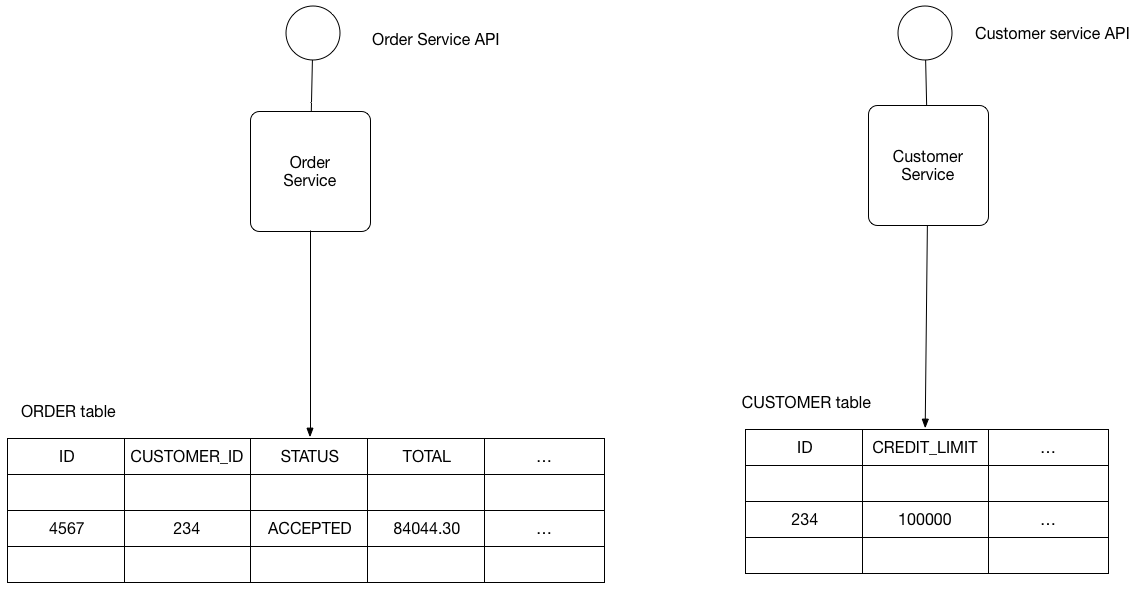
\includegraphics[width=13cm]{images/shared_database.png}}	
		\captionof{figure}{\textit{Shared database.}}
	\end{minipage}
\end{adjustbox}\\

\textbf{Shared database.} Model yang pertama adalah database yang di \textit{share} untuk diakses oleh beberapa service. Modul \textit{order} bisa langsung mengakses table \textit{customer} untuk mendapatkan limit kredit \textit{customer} tersebut. Model ini dapat menjadi pilihan ketika \textit{developer} ingin model yang familiar dan tegas untuk menjaga konsistensi data. Model \textit{shared database} memiliki beberapa kelemahan, antara lain :
\begin{enumerate}[leftmargin=*]
	\item \textit{Development time coupling.} Modul \textit{order} harus tahu apabila terjadi perubahan pada \textit{schema customer}, hal ini menjadikan kedua modul menjadi memiliki ketergantungan. Hal ini akan memperlambat proses \textit{development}.
	\item \textit{Runtime coupling.} Karena beberapa service dapat mengakses database yang sama, terdapat potensi mengganggu proses yang lain, misalnya ketika modul \textit{customer} sedang melakukan \textit{update} terhadap \textit{customer} dengan id 234 untuk merubah kredit limit, maka modul \textit{order} harus menunggu sampai \textit{update customer} selesai dilakukan karena \textit{customer} dengan id 234 akan di \textit{block} sementara waktu.
\end{enumerate}
\textbf{Database per service}. Pattern database yang kedua menjadikan sebuah table menjadi \textit{private} hanya untuk 1 buah service dan hanya dapat diakses via API, service lain tidak bisa mengakses database tersebut. Kelebihan dari model ini adalah menjadikan service lebih \textit{loose coupled}, tingkat ketergantungan antar service rendah. Tiap service pun dapat memiliki database yang cocok untuk dirinya sendiri. Namun model database ini memiliki beberapa kesulitan, antara lain :
\begin{enumerate}[leftmargin=*]
	\item Mengimplementasikan proses bisnis yang melibatkan banyak service menjad lebih sulit, dan lebih baik dihindari karena akan menemukan kesulitan di integritas data, terutama database modern (NoSQL). Solusi terbaik adalah dengan menggunakan konsep SAGA pattern (dibahas pada point berikutnya), yang menjalankan \textit{event} ketika ada perubahan data. Service lain yang men-\textit{subscribe event} tersebut akan merespon dan melakukan \textit{update} \cite{6}.
	\item Mengimplementasi \textit{query} yang menggabungkan data dari banyak database akan lebih sulit \cite{6}.
\end{enumerate}
\subsection{\textit{API Composition}}
Ketika mengaplikasikan arsitektur microservice menggunakan pattern \textit{database per service}, praktis implementasi dari \textit{straightforward query} yang menggabungkan data lebih dari satu tabel tidak dapat dilakukan lagi, karena tabel dalam database terpisah di berbagai lokasi service. Solusi untuk dapat mengatasi permasalahan ini adalah dengan menggunakan \textit{API Composition}. Ide dari konsep ini adalah menggabungkan data hasil service dan melakukan \textit{in-memory} join di level sistem. Namun kelemahan dari metode ini adalah menyebabkan data join yang besar dalam \textit{memory} system. Untuk menangani masalah tersebut, dapat dilakukan dengan meningkatkan performa \textit{hardware}, misal menambah \textit{core} dari \textit{processor} dan menambah \textit{memory} sistem \cite{6}.
\subsection{Dekomposisi Modul}
Tujuan dari dekomposisi modul ini adalah menemukan service terkecil penyusun aplikasi. Dengan memisahkan modul menjadi sebuah service tunggal, menjadikan aplikasi lebih mandiri dan mudah untuk di koordinasikan dalam tim, yang dapat mempercepat proses \textit{development}. Tujuan yang lebih besar lagi adalah menghindari perubahan besar pada aplikasi ketika ada proses bisnis yang berubah. Dengan mendekomposisi modul, akan membantu untuk memastikan hanya ada sebuah service saja yang akan terkena dampaknya.\\
Tantangan yang didapat ketika hendak melakukan dekomposisi modul adalah :
\begin{enumerate}[leftmargin=*]
	\item Rancangan arsitektur service yang baru harus stabil.
	\item Sebuah service harus terdiri dari susunan \textit{functions} yang erat fungsinya.
	\item Service harus memastikan tidak melanggar \textit{Common Closure Principle}, yaitu apabila terjadi perubahan tidak akan melibatkan \textit{package} lain.
	\item Setiap service sebagai API yang terenkapsulasi dari pengguna. Segala perubahan tidak boleh memberikan dampak secara langsung pada pengguna.
	\item Sebuah service harus cukup kecil untuk ditangani oleh tim yang terdiri dari 6-10 orang.
	\item Service harus bisa di tes, dan setiap tim harus dapat melakukan proses \textit{develop} dan \textit{deploy} tanpa banyak interaksi dengan tim lain.
\end{enumerate}
Terdapat 2 metode dalam mendekomposisi modul aplikasi, yaitu berdasarkan subdomain dan berdasarkan proses bisnis yang dilakukan \cite{6}.\\
\textbf{Dekomposisi berdasarkan subdomain.} Apabila aplikasi yang dibentuk terpisah berdasarkan \textit{domain-driven design} (DDD) atau disebut juga subdomain, maka metode ini dapat lebih mudah digunakan. DDD memisahkan aplikasi berdasarkan kebutuhannya dan membentuk sebuah subdomain sendiri, setiap subdomain bertanggung jawab untuk menangani proses bisnis yang berbeda.Subdomain dapat diklasifikasikan sebagai berikut :
\begin{enumerate}[leftmargin=*]
	\item \textit{Core} – kunci pembeda dari proses bisnis dan menjadi bagian yang sangat penting dari sebuah aplikasi.
	\item \textit{Supporting} – berhubungan dengan proses bisnis namun bukan menjadi pembeda.
	\item \textit{Generic} – tidak berhubungan dengan proses bisnis dan biasanya hanya menjadi proses pendukung saja.
\end{enumerate}
Kelebihan dari metode ini antara lain:
\begin{enumerate}[leftmargin=*]
	\item Arsitektur service baru yang stabil, karena subdomain sendiri secara relatif sudah stabil.
	\item Service yang dibentuk akan cenderung memenuhi \textit{loosely coupled} dan \textit{cohesive}.
\end{enumerate}
Masalah yang dihadapi dari metode ini antara lain:
\begin{enumerate}[leftmargin=*]
	\item Sulit diterapkan untuk aplikasi yang tidak \textit{domain-driven} atau aplikasi yang memiliki keterikatan modul yang kuat.
\end{enumerate}
\textbf{Dekomposisi berdasarkan proses bisnis.} Pattern alternatif yang lain adalah mendefinisikan service berdasarkan kemampuan bisnis. Kemammpuan bisnis adalah proses yang dilakukan untuk menghasilkan sebuah nilai. Kemampuan bisnis biasanya berhubungan dengan objek bisnis. Misalnya \textit{order management} bertanggung jawab untuk \textit{orders}, \textit{customer management} bertanggung jawab untuk \textit{customer}.  Kemampuan bisnis biasanya tersusun menjadi hirarki multi level, misalnya untuk aplikasi perusahaan memiliki \textit{product/service development}, setelah itu ada \textit{product/service delivery}, lalu diikuti dengan \textit{aftersale service} \cite{6}
Kelebihan dari metode ini antara lain:
\begin{enumerate}[leftmargin=*]
	\item Arsitektur service baru yang stabil, karena kemampuan bisnis pun relatif sudah stabil.
	\item Service yang dibentuk akan memenuhi konsep \textit{loosely coupled} dan \textit{cohesive}.
\end{enumerate}
Masalah yang akan dihadapi dari metode ini antara lain:
\begin{enumerate}[leftmargin=*]
	\item Sulit untuk mengidenfitikasi kemampuan bisnis aplikasi. Identifikasi pembentukan service membutuhkan pemahaman dari proses bisnis, maka harus dilakukan analisa mendalam dari tujuan perusahaan, struktur, dan cakupan area. Analisa dapat dilakukan pertama-tama dari struktur organisasi, karena perbedaan grup dalam organisasi berkaitan dengan kemampuan bisnis dari grup tersebut.
\end{enumerate}
\subsection{Service Deployment}
Setelah mengindentifikasi dan membentuk service, tahap selanjutnya yang akan dilakukan adalah melakukan \textit{deployment} service untuk nantinya digunakan. Tiap service sendiri bisa ditulis menggunakan bahasa dan framework yang berbeda-beda, namun secara mandiri harus \textit{deployable} dan \textit{scalable}. Dalam beberapa kasus, akan terdapat set service yang harus terisolasi dari service lainnya. Kebutuhan lainnya adalah adanya keperluan untuk dapat memantau penggunaan \textit{resources} (CPU dan memori) yang digunakan oleh service dan memantau dengan mudah sifat dan kegunaan dari service tersebut. Semua kebutuhan ini juga harus sebanding dengan biaya yang dikeluarkan.\\
Terdapat beberapa metode \textit{deployment} yang dapat dilakukan, tiap metode cocok digunakan sesuai dengan kebutuhan dari \textit{deployment} itu sendiri. Point berikutnya akan menjelaskan metode-metode \textit{deployment} service.
\begin{enumerate}[leftmargin=*]
	\item \textbf{Multiple service instances per host.}\\
	Metode \textit{deployment} ini cocok digunakan apabila service yang terbentuk tidak banyak dan adanya kebutuhan untuk menghemat penggunaan sumber daya. Set service yang terbentuk disimpan dalam sebuah host (fisik atau \textit{virtual machine}). Terdapat 2 cara dalam melakukan \textit{deploy} set service dalam sebuah host. Pertama, \textit{deploy} set-set service tersebut sebagai JVM, misalnya dengan Tomcat atau Jetty untuk sebuah set service. Kedua adalah melakukan \textit{deploy} semua set service dalam sebuah JVM yang sama, mislanya sebagai web aplikasi \cite{6}.\\
	Metode deployment ini juga terdapat beberapa kelemahan, antara lain:
	\begin{enumerate}[leftmargin=*]
		\item Beresiko terjadi konflik terhadap kebutuhan sumber daya (memori dan CPU).
		\item Beresiko terjadi konflik versi dependency.
		\item Sulit untuk membatasi konsumsi sumber daya yang digunakan sebuah service (berhubungan dengan point pertama).
		\item Apabila banyak set service di deploy dalam sebuah mesin yang sama, maka akan sulit untuk memonitor konsumsi sumber daya dari tiap service, karena sulit untuk melakukan isolasi terhadap service.
	\end{enumerate}
	\item \textbf{Single service instance per host.}\\
	Pilihan yang kedua adalah setiap service memiliki hostnya sendiri. Dengan menerapkan pattern ini, setiap service akan terisolasi dari yang lainnya, serta tidak akan ada resiko konflik akan sumber daya dan dependency. Setiap service lebih mudah untuk dimonitor dan dikelola. Namun kekurangan dari patern ini apabila dibandingkan dengan multiple service per host adalah kurangnya efisiensi penggunaan sumber daya, karena bisa jadi akan ada banyak host yang digunakan \cite{9}
	
\begin{adjustbox}{width=1\textwidth}
	\centering
	\begin{minipage}{\linewidth}
		\framebox[\textwidth]{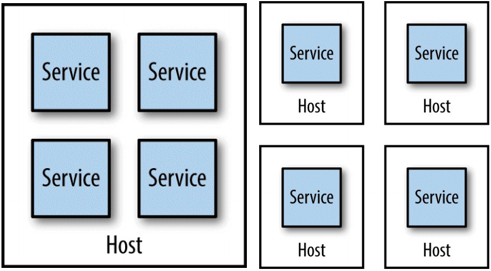
\includegraphics[width=8cm]{images/service_deployment.png}}	
		\captionof{figure}{\textit{Banyak service per host dan satu service per host.}}
	\end{minipage}
\end{adjustbox}\\
	\item \textbf{Service instance per container.}\\
	Apabila masing-masing service dibuat dengan bahasa atau framework yang berbeda, maka proses \textit{deployment} dari setiap service akan berbeda-beda pula. Dengan menggunakan \textit{container}, semua detail teknologi yang digunakan oleh setiap service akan dibuat terenkapsulasi dari service lain. \textit{Container} juga menspesifikasikan dengan jelas bagaimana proses \textit{deployment} yang harus dilakukan dalam sebuah mesin, sehingga ketika sebuah aplikasi hendak dijalankan dalam mesin yang berbeda, user tidak perlu tahu proses apa saja yang harus dilakukan [9].  Contoh dari \textit{container} adalah Docker, namun Docker tidak bisa melakukan \textit{deployment} dalam banyak mesin. Maka dari itu Google mengembangkan \textit{tools} yang bernama Kubernetes, Kubernetes memungkinkan agar Docker bisa dalam satu saat bersamaan dijalankan dalam banyak mesin sekaligus \cite{9}
	
\begin{adjustbox}{width=1\textwidth}
	\centering
	\begin{minipage}{\linewidth}
		\framebox[\textwidth]{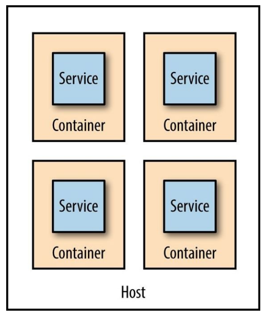
\includegraphics[width=5cm]{images/container_deployment.png}}	
		\captionof{figure}{\textit{Menggunakan container untuk \textit{deployment}.}}
	\end{minipage}
\end{adjustbox}\\
	\item \textbf{Serverless deployment.}\\
	Ide dari serverless deployment adalah mengurangi interaksi dari pengguna dengan server. Segala hal yang berhubungan dengan infrastruktur server disembunyikan dari pengguna. Pengguna hanya dikenakan biaya penyewaan server saja, namun tidak perlu lagi melakukan pengaturan apapun pada server. Untuk melakukan deployment, pengguna meembuat package dari kode (misalnya ZIP file), lalu melakukan upload kepada penyedia jasa server dan melakukan pengaturan performa. Ada beberapa penyedia jasa lingkungan serverless, misalnya AWS Lambda, Google Cloud Function, Microsoft Azure \cite{6}.\\
	Kelebihan dari penggunaan serverless ini antara lain:
	\begin{enumerate}[leftmargin=*]
		\item Tidak perlu membuang-buang waktu untuk mengurus menejemen infrastruktur low-level. Pengguna bisa lebih fokus untuk mengembangkan aplikasinya saja.
		\item Arsitektur dari serverless sangat elastis. Server secara otomatis menghitung beban dari service yang digunakan agar tidak ada resource yang terbuang.
	\end{enumerate}
	Kekurangan dari serverless antara lain:
	\begin{enumerate}[leftmargin=*]
		\item Adanya batasan lingkungan, misalnya server hanya bisa support untuk beberapa bahasa saja.
	\end{enumerate}
\end{enumerate}
\subsection{Metode Berkomunikasi Antar Service}
Dengan memiliki modul service yang berbeda-beda, timbul sebuah masalah yang berkaitan dengan pertukaran informasi yang berasal dari banyak service. \textit{Remote Procedure Invocation} (RPI) adalah protocol yang menyediakan teknik komunikasi antara service yang berbeda lokasi. Teknologi RPI ini ada yang menggunakan kode biner sebagai format pertukaran data, ada pula yang menggunakan format pesan XML seperti SOAP. Implementasi RPI ini berguna untuk mendapatkan data dengan sangat cepat yang dikirimkan melalui jaringan, hal yang menjadi keuntungan utama dari RPI adalah kemudahan penggunaannya. Contoh RPI lain yang menjadi fokus disini adalah Representational State Transfer (REST), point berikutnya akan menjelaskan mengapa REST menjadi pilihan terbaik untuk menangani proses komunikasi di microservice \cite{9}.

\textbf{Representational State Transfer (REST).} REST adalah standar arsitektur web yang menggunakan protokol HTTP. HTTP sendiri mempunyai kemampuan yang sangat cocok untuk REST, salah satunya HTTP faham apa yang harus dilakukan apabila menerima perintah GET, POST, PUT dari REST. Kelebihan penting yang dimiliki REST adalah pengguna bisa menghindari kontak langsung dari pengguna dengan server secara langsung. Konsep ini kemudian disebut sebagai \textit{hypermedia as the engine of application state} (HATEOAS). \textit{Hypermedia} adalah konsep dimana sebuah konten mempunyai link yang berhubungan dengan konten lainnya yang bisa berupa berbagai format (text, gambar, suara) \cite{9}. Ide dari HATEOAS adalah \textit{client} berhubungan dengan server hanya dengan menggunakan \textit{link} yang telah disediakan. 
Misalnya seperti gambar 2.6 dibawah. Ketika pengguna ingin mengubah data \textit{account}, maka pengguna akan mengirimkan \textit{request} pada \textit{account service}, \textit{account service} dengan logic yang dimilikinya akan menentukan apakah request tersebut dapat diterima. \textit{Account service} disini menjaga semua interaksi yang berhubungan dengan data \textit{account} itu sendiri. \textit{Client} tidak perlu tahu dan tidak perlu beradaptasi apabila terjadi perubahan pada server. \textit{Client} akan merasakan perubahan hanya apabila terjadi perubahan sifat atau ketika hilangnya kontrol yang merepresentasikan \textit{account}. Format data yang dikirimkan REST di HTTP dapat beragam, namun yang paling populer adalah format JSON, karena JSON mudah dimengerti dan mudah dikonsumsi langsung. REST pada HTTP sangat baik untuk diimplementasikan pada interaksi \textit{sevice-to-service} \cite{9}\\

\begin{adjustbox}{width=1\textwidth}
	\centering
	\begin{minipage}{\linewidth}
		\framebox[\textwidth]{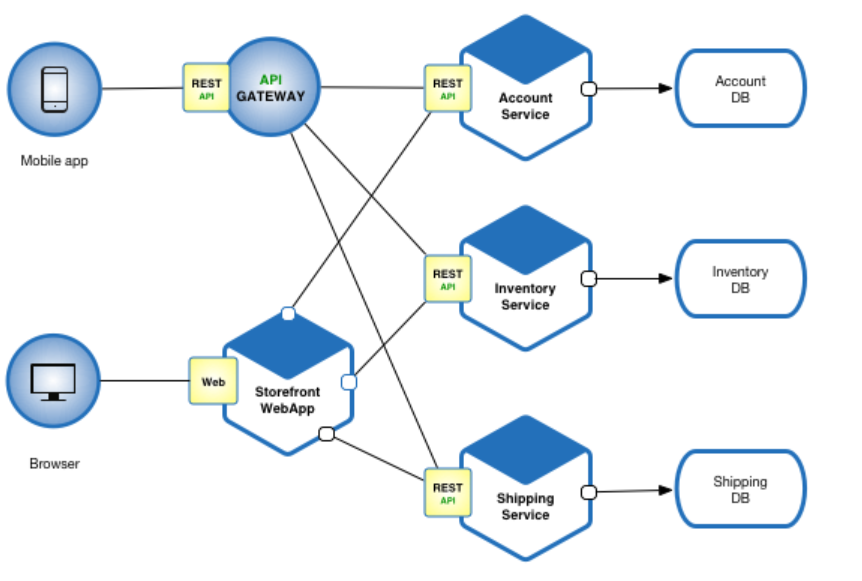
\includegraphics[width=12cm]{images/rest_example.png}}	
		\captionof{figure}{\textit{Contoh pemanfaatan REST sebagai media user-server}}
	\end{minipage}
\end{adjustbox}\\
\section{Strategi Pengujian}
Strategi pengujian berguna untuk memberikan gambaran dari test yang akan dilakukan terhadap \textit{software}. Testing ini berguna untuk memberi tahu kepada proyek menejer, tester, dan tim pengembang apabila ditemukannya masalah dalam \textit{software}. Strategi pengujian ini termasuk tujuan dari test, metode yang digunakan, sumber daya yang digunakan, juga lingkungan ketika menjalankan proyek. Test strategi mendeskripsikan seberapa tinggi resiko kesalahan (kegagalan) yang dapat terjadi \cite{12}. 
\subsection{Pengujian Arsitektur Microservice}
Uji kelayakan arsitektur microservice menurut Martin Fowler adalah dengan melakukan 5 test yang mirip dengan software testing pada umumnya, test tersebut antara lain adalah:
\begin{enumerate}[leftmargin=*]
	\item \textit{Unit Testing}. Bagian terkecil dalam software yang ditest untuk menentukan apakah unit tersebut bekerja sesuai harapan. Umumnya, unit yang dimaksud adalah kelas penyusun atau grup kecil yang menghubungkan kelas-kelas tersebut dan method yang terdapat dalam kelas.
	\item \textit{Integration Testing}. Goal dari test ini adalah membuktikan bahwa tidak terdapat masalah dari komunikasi dan interaksi dari setiap unit.
	\item \textit{Component Testing.} Komponen membatasi lingkup sebuah software. Dalam 1 buah komponen, dapat terdiri dari beberapa integrasi yang terjadi antara unit kelas.
	\item \textit{Contract testing.} Test yang memverifikasi bahwa pihak luar yang mengakses sebuah service akan mendapatkan hasil yang sesuai dengan harapan.
	\item \textit{End-to-end Testing.} Memverifikasi bahwa sistem memenuhi telah berhasil memenuhi kebutuhan dan sesuai dengan rancangan goal. Test dilakukan dari awal sampai dengan output yang dihasilkan. 
\end{enumerate}
\begin{adjustbox}{width=1\textwidth}
	\centering
	\begin{minipage}{\linewidth}
		\framebox[\textwidth]{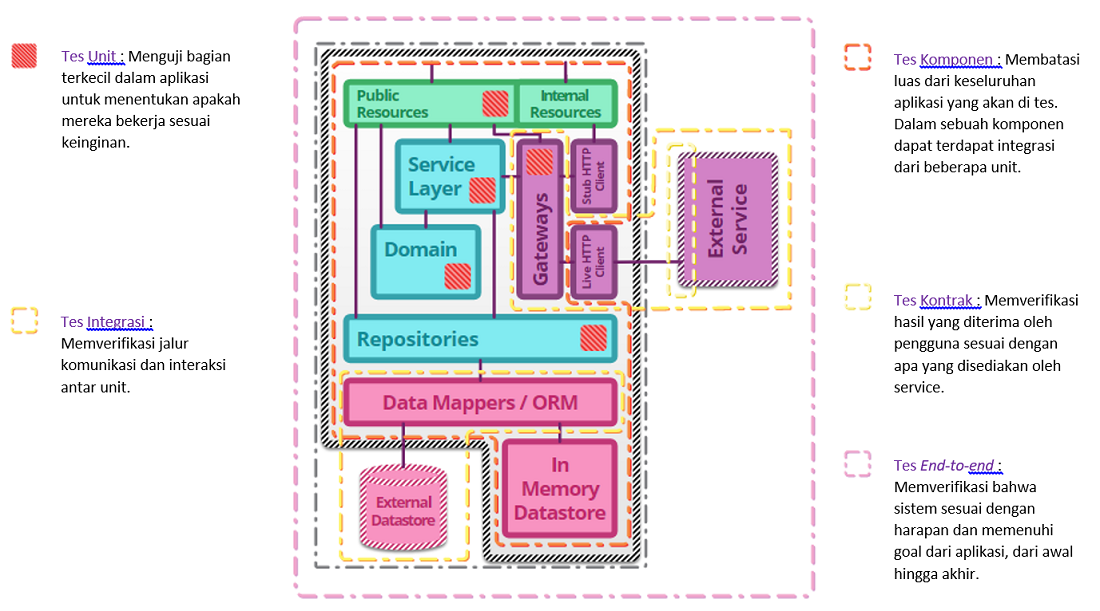
\includegraphics[width=13cm]{images/software_test.png}}	
		\captionof{figure}{\textit{Testing pada software microservice}}
	\end{minipage}
\end{adjustbox}\\

Tujuan utama dari testing yang pertama adalah memastikan bahwa fungsi bisnis dari arsitektur yang baru sudah memenuhi \textit{requirement} yang sama dengan arsitektur monolitik sebelumnya.
\subsection{Uji Perbandingan Performa}
Test kedua adalah menunjukan bahwa performa dari arsitektur microservice akan memberikan hasil yang lebih baik dari monolitk. Strategi pengujian yang akan dilakukan adalah dengan membuat point-point pembanding yang akan diuji, kemudian dari point tersebut akan dibuat \textit{test-plan} masing-masing ang terdiri dari sekitar 1-3 buah \textit{test-plan}. Hasil tes kemudian akan disimpan dalam dokumen berupa \textit{matrix traceability}.
Menurut Paulo Merson (Software Architecture di TCU; SOA/microservice trainer dan consultan), point pembanding tersebut adalah \cite{12}:
\begin{enumerate}[leftmargin=*]
	\item \textit{Deployability}. Lebih agile untuk meluncurkan versi terbaru karena siklus \textit{build, test, build} yang lebih pendek. Tingkat fleksibilitas yang lebih tinggi untuk menggunakan layanan keamanan, replikasi, persistensi, dan konfigurasi pemantauan.
	\item \textit{Reliability}. Kesalahan dalam microservice hanya akan berpengaruh pada microservice itu sendiri dan konsumennya, sedangkan dalam model monolitik kesalahan layanan dapat merusak seluruh sistem monolitik.
	\item \textit{Availability}. Waktu \textit{downtime} yang dibutuhkan ketika ingin mengeluarkan versi terbaru dari microservice lebih sedikit dibandingkan monolitik.
	\item \textit{Scalability}. Setiap microservice dapat diskalakan secara terpisah menggunakan \textit{pool, cluster, grid}. Karakter menyebar membuat microservice lebih fleksibel dibandingkan dengan monolitik.
	\item \textit{Modifiability and Management}. Sifat fleksibel untuk menggunakan \textit{framework, libraries}, dan sumber data baru karena ditunjang sifat \textit{loose-coupled} yang dimiliki microservice, modular komponen hanya dapat diakses oleh contracts (pihak yang berhak), dan sifat yang cenderung tidak mudah berubah menjadi software besar yang sulit ditangani. Upaya pengembangan aplikasi juga dapat dibagi dalam tim yang lebih kecil dan bekerja lebih mandiri. 
\end{enumerate}
\newpage
	\setcounter{page}{1}
	%-----------------------------------------------------------------------------%
\chapter{ANALISIS DAN PERANCANGAN SISTEM}

%-----------------------------------------------------------------------------%

%
\vspace{4.5pt}

Bab ini menjelaskan analisis masalah beserta pendekatan dan alur kerja dari aplikasi yang akan dikembangkan, dimulai dari \textit{preprocessing}, implementasi metode dan hasil yang ditampilkan.
\section{Analisis Masalah}
Dalam penelitian ini, penulis akan menggunakan data berupa \textit{tweet} dari media sosial Twitter untuk data \textit{training} dan data \textit{testing}. Penulis memilih media sosial Twitter sebagai objek penelitian, karena Twitter memiliki fitur \textit{hashtag} yang dapat digunakan untuk mendapatkan data sarkasme, yang kemunculannya sedikit. Selain itu, pada tahun 2011 tercatat ada 200 juta \textit{tweet} setiap harinya. Penulis akan menggunakan klasifikasi \textit{Support Vector Machine} (SVM) pada pengembangan \textit{sistem} analisis sentimen ini. \textit{Kernel} SVM yang dipilih adalah linear, karena jumlah fitur lebih banyak dibanding jumlah data. Data diambil dengan \textit{scraping} html pada halaman Twitter menggunakan \textit{library} Python, yaitu Twitter-scraper. Data diambil berdasarkan pencarian pada Twitter dengan berbagai \textit{keyword}. \textit{Keyword} yang digunakan adalah "DPR", "film", "sekolah" dan "internet" untuk mendapatkan data dengan label positif, negatif 
dan netral. Sedangkan data dengan label sarkasme diambil dengan menggunakan \textit{keyword} seperti "DPR \#sarkasme", "film \#sarkasme", "sekolah \#sarkasme", dan "internet \#sarkasme". Digunakannya \textit{keyword} tersebut karena \textit{keyword} 
tersebut memiliki cukup banyak data sarkasme, dengan 13 teks sarkasme pada \textit{keyword }DPR, 3 teks sarkasme pada \textit{keyword} film, 12 teks sarkasme pada \textit{keyword} sekolah dan 7 teks sarkasme pada \textit{keyword} internet. Dalam penelitian ini akan dilakukan klasifikasi dengan 2 teknik klasifikasi, yaitu \textit{levelled method} dan \textit{direct method} \cite{5}. Pengklasifikasian akan menganggap teks sarkasme sebagai positif sarkasme, karena teks sarkasme cenderung terlihat seperti teks positif, namun bernilai negatif \cite{5}. Berikut ini adalah \textit{flowchart }
proses klasifikasi dengan \textit{levelled method}:

\begin{adjustbox}{width=1\textwidth}
\begin{minipage}{\linewidth}
	\framebox[\textwidth]{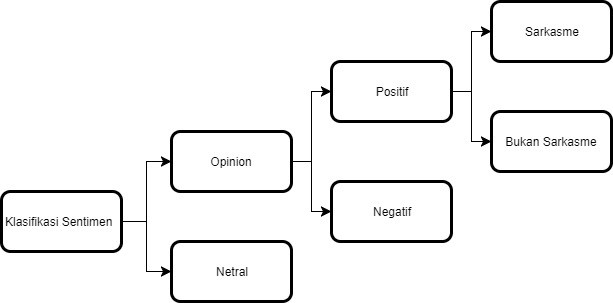
\includegraphics[width=10cm]{images/levelled_method.jpg}}	
	\captionof{figure}{Klasifikasi dengan \textit{Levelled Method}}
\end{minipage}
\end{adjustbox}

Berikut ini adalah \textit{flowchart }proses klasifikasi dengan \textit{direct method}:

\begin{adjustbox}{width=1\textwidth}
\begin{minipage}{\linewidth}
	\framebox[\textwidth]{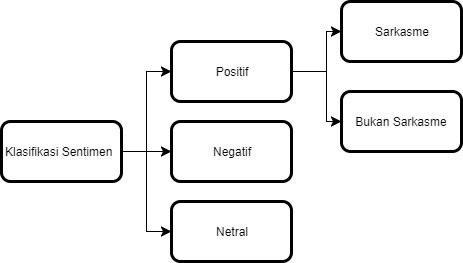
\includegraphics[width=10cm]{images/direct_method.jpg}}	
	\captionof{figure}{Klasifikasi dengan \textit{Levelled Method}}
\end{minipage}
\end{adjustbox}

Klasifikasi \textit{levelled method} dan \textit{direct method }akan membangun sebanyak 4 model. Berikut ini adalah model yang diperlukan untuk klasifikasi \textit{levelled method }dan \textit{direct method}:

\begin{enumerate}[leftmargin=*]
	\item Model 1\ \ \ \ : kelas netral atau bukan netral.
	\item Model 2\ \ \ \ : kelas positif atau bukan positif.
	\item Model 3\ \ \ \ : kelas negatif atau bukan negatif.
	\item Model 4\ \ \ \ : kelas sarkasme atau bukan sarkasme.
\end{enumerate}

Pada klasifikasi \textit{levelled method }akan dilakukan klasifikasi teks termasuk sebagai kelas netral atau kelas opini. Jika teks merupakan kelas opini, maka akan diklasifikasikan menjadi teks positif atau negatif. Jika hasilnya kelas positif, maka akan diklasifikan menjadi teks sarkasme atau non-sarkasme. Sedangkan pada klasifikasi \textit{direct method} teks akan langsung diklasifikasikan sebagai 3 kelas, yaitu positif, negatif atau netral. Jika teks merupakan positif, maka akan diklasifikasikan sebagai sarkasme atau non-sarkasme. Penelitian ini akan membandingkan akurasi klasifikasi \textit{levelled method} dan \textit{direct method}.

Data \textit{tweet} yang dikumpulkan akan diberi label secara manual. Data \textit{tweet} yang diambil tersebut diberi label sebagai positif, negatif, netral, sarkasme. Salah satu fitur yang dianggap membantu dalam penentuan teks sarkasme adalah menggunakan fitur seperti \textit{emoticon}, kemunculan kata \textit{adjective }dan \textit{adverb, }kemunculan \textit{interjection }dan penggunaan \textit{punctuation }\cite{5}. Fitur-fitur yang akan digunakan pada penelitian ini adalah \textit{unigram,} \textit{interjection}, \textit{question word,} \textit{sentiment score, capitalization},
\textit{ topic}, \textit{part of speech} dan \textit{punctuation-based}. Fitur \textit{unigram }lebih dipilih dibanding \textit{bigram},\textit{ }karena kata-kata pada media social terlalu beragam, sehingga sulit untuk menemukan kata yang sama jika 
menggunakan \textit{bigram}. Berikut ini adalah contoh teks yang akan menganggap sebuah kata beda jika menggunakan \textit{bigram}:

\begin{enumerate}[leftmargin=*]
	\item Se7...kalau boleh setiap hari kemerdekaan WAJIB TAYANG \textbf{DI 
		SEKOLAH}
	\item Ceritanya menarik. Karakternya juga unik. Salah satu karakter 
	favorit, Endong. Aktingnya cukup keren. Sangat cocok di tonton \textbf{
		anak sekolah}.
	\item Tiap sore \textbf{pulang} \textbf{sekolah} ngarepin paket 
	dating
\end{enumerate}

Berdasarkan data di atas, jika menggunakan \textit{bigram}, akan menghasilkan token ["tayang sekolah"], ["anak sekolah"], dan ["pulang sekolah"]. Hal tersebut menyebabkan setiap token tersebut akan dianggap berbeda dan nilai fitur tidak bagus. Kata "di" pada teks 1 dihapus, karena kata "di" tidak memiliki makna, oleh karena itu fitur kata \textit{bigram} menjadi ["tayang sekolah"]. Sedangkan jika menggunakan \textit{unigram}, akan menghasilkan token ["tayang", "sekolah"], ["anak", "sekolah"], dan ["pulang", "sekolah"]. Sehingga kata "sekolah" dapat memberikan nilai fitur yang lebih baik karena kemunculannya adalah 3.

\pagebreak

\section{Kerangka Pemikiran}
Berikut ini adalah kerangka pemikiran dari metode yang diusulkan untuk 
melakukan klasifikasi:

\begin{adjustbox}{width=1\textwidth}
\begin{minipage}{\linewidth}
	\framebox[\textwidth]{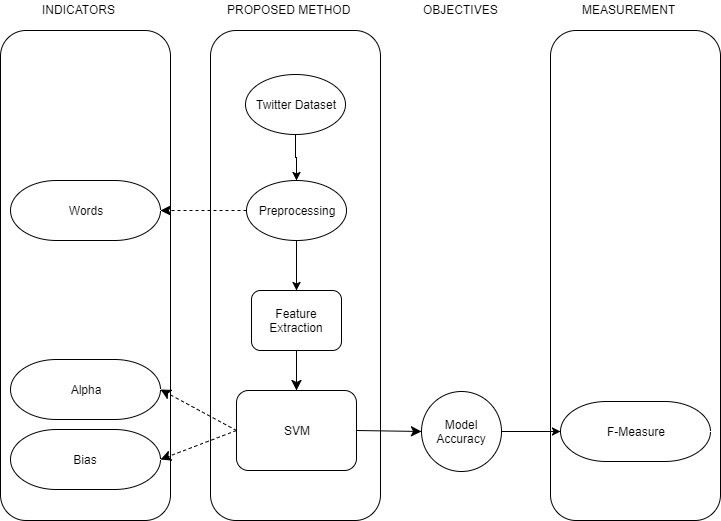
\includegraphics[width=10cm,height=8cm]{images/kerangka_pemikiran.jpg}}	
	\captionof{figure}{Kerangka kerja klasifikasi teks}
\end{minipage}
\end{adjustbox}

Sistem akan dimulai dari masukan data Twitter. Kemudian melakukan proses \textit{text preprocessing} dengan menggunakan data Twitter yang sudah diberi label. Tahap selanjutnya setelah \textit{preprocessing} adalah melakukan \textit{feature extraction}. Hasil \textit{feature extraction }akan digunakan untuk pemodelan klasifikasi SVM. Setelah mendapatkan modelnya, maka dapat dihitung akurasinya dengan \textit{f-measure}.
 
\section{\textit{Flowchart} Sistem Analisis Sentimen}
Berikut adalah flowchart untuk sistem analisis sentimen dalam penelitian 
ini:

\begin{adjustbox}{width=1\textwidth}
\noindent\begin{minipage}{\linewidth}
	\framebox[\textwidth]{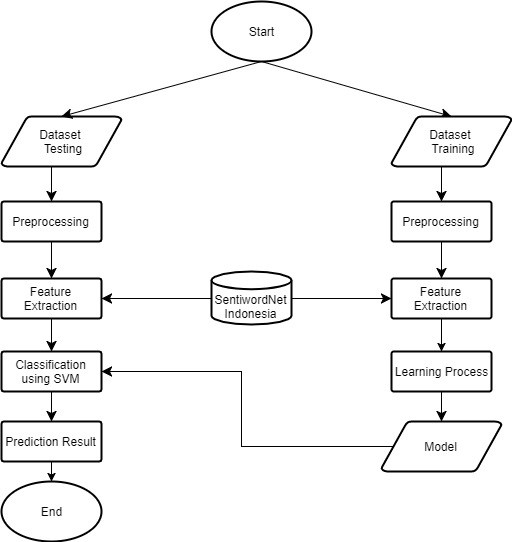
\includegraphics[width=10cm]{images/flowchart.jpg}}	
	\captionof{figure}{\textit{Flowchart} Sistem Analisis Sentimen}
\end{minipage}
\end{adjustbox}

Alur proses sistem dimulai dari data \textit{training}. Kemudian dilanjutkan dengan \textit{preprocessing}. Setelah itu, data \textit{training} yang sudah di \textit{preprocessing }akan masuk ke tahap \textit{feature extraction} untuk mendapatkan informasi dari setiap teks. \textit{Feature extraction }akan menggunakan data SentiWordNet untuk mendapatkan fitur nilai sentimen dari sebuah teks. Kemudian melakukan \textit{learning process} untuk menghasilkan model klasifikasi SVM. Setelah model didapatkan, data \textit{testing} dapat melakukan tahap-tahap seperti pada data \textit{training}, yaitu \textit{preprocessing }dan\textit{ feature extraction}. Setelah mendapat fitur dari data \textit{testing}, selanjutnya dapat melakukan klasifikasi teks dengan model yang sudah melalui \textit{learning process}. 

\subsection{Analisis Data}
Dalam penelitian ini, akan digunakan 236 data \textit{tweet} yang sudah diberi kelas pada setiap \textit{tweet}. Kelas tersebut dibagi menjadi 4 kelas yaitu, kelas positif, kelas negatif, kelas netral dan kelas sarkasme. Selain itu, akan digunakan 177 data \textit{tweet} sebagai data training, dan 59 data \textit{tweet} sebagai data \textit{testing}. Berikut contoh dari data \textit{tweet} yang akan digunakan:

\begin{enumerate}[leftmargin=*]
	\item Kelas Positif\\
	Sukses untuk pak @aniesbaswedan, stop reklamasi !!
	\item Kelas Negatif\\
	Anggota DPR skrg tidak mementingkan rakyat.
	\item Kelas Netral\\
	Menurut Netizen, Apakah DPR RI/DPRD sudah mewakili aspirasi rakyat?
	\item Kelas Sarkasme\\
	Semoga FH dan FZ ada di DPR selamanya.. krn sepi dunia kalau gak ada mereka.. :)
\end{enumerate}

\noindent Karakteristik data yang digunakan:
\begin{enumerate}[leftmargin=*]
	\item Semua sarkasme akan dianggap sebagai sarkasme positif.
	\item Jika ada perbandingan pada sebuah kalimat, pemberian label 
	berdasarkan kalimat yang lebih memberi nilai positif maupun negatif, 
	sebagai contoh \textit{tweet} "Tapi, penilaian sy kinerja 
	pemerintahan dan kpk lebih baik daripada yang di dpr", teks tersebut 
	akan diberi label positif.
\end{enumerate}
		
\subsection{\textit{Text Preprocessing}}
Sebelum melakukan ekstraksi fitur, akan dilakukan \textit{text} \textit{preprocessing }pada data \textit{training} dan data \textit{testing}. \textit{Text preprocessing }dilakukan untuk mengurangi \textit{noise}, dan mengurangi kata-kata non-formal. Beberapa metode untuk menangani \textit{noise} atau kata-kata non-formal pada \textit{text preprocessing }seperti \textit{case folding, remove hashtag}, URL dan \textit{mention}, \textit{remove punctuation}, \textit{tokenization}, \textit{misuse of word}, \textit{abbreviation word}, \textit{stopword removal}, dan \textit{stemming}. Berikut ini adalah \textit{flowchart text preprocessing} yang akan dilakukan:

\begin{adjustbox}{width=1\textwidth}
\begin{minipage}{\linewidth}
	\framebox[\textwidth]{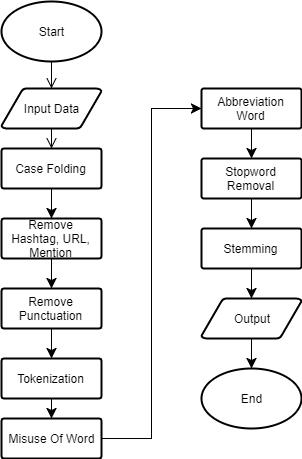
\includegraphics[width=10cm,height=10cm]{images/text_preprocessing.png}}	
	\captionof{figure}{\textit{Flowchart Text Preprocessing}}
\end{minipage}
\end{adjustbox}

\subsubsection{\textit{Case Folding}}
Pada tahap \textit{Case Folding, }kalimat pada teks akan diubah menjadi huruf kecil. \textit{Case folding }dilakukan untuk mengatasi masalah kata yang sama, hanya berbeda huruf kapital.

\begin{table}[H]
	\caption{Tabel Hasil \textit{Case Folding}}
	\centering
	\small
	\begin{adjustbox}{width=1\textwidth}
	\begin{tabular}{|p{6.50cm}|p{6.50cm}|}
		\hline
		\textbf{Teks} & \textbf{Hasil} \\
		\hline
		\textbf{BPK} terbaik. \textbf{BI} terbaik. \textbf{DPR} ter? \textbf{@Fahrihamzah} ter? \textbf{Mandi} dlu \textbf{Ooom!} 
		& \textbf{bpk} terbaik. \textbf{bi} terbaik. \textbf{dpr} ter? \textbf{@fahrihamzah} ter? \textbf{mandi} dlu \textbf{ooom!} \\
		\hline
	\end{tabular}
	\end{adjustbox}
\end{table}
\subsubsection{\textit{Remove Hashtag}, URL, \textit{Mention}}
Pada tahap ini, semua \textit{hashtag}, URL, \textit{mention} akan dihapus dari teks. Penghapusan ini dilakukan karena dalam teks sarkasme sering terdapat \textit{hashtag} \#sarkasme, hal ini dapat membantu dalam sebuah fitur jika tidak menghapusnya. Namun setiap teks yang memiliki \textit{hashtag} \#sarkasme, tidak menentukan bahwa sebuah 
teks adalah sarkasme, sehingga \textit{hashtag} akan dihapus. Berikut ini adalah contoh hasil \textit{remove hashtag}, URL, dan \textit{mention}:
\begin{table}[H]
	\caption{Tabel Hasil \textit{Remove Hashtag}, URL, \textit{Mention}}
	\centering
	\small
	\begin{adjustbox}{width=1\textwidth}
	\begin{tabular}{|p{6.50cm}|p{6.50cm}|}
		\hline
		\textbf{Teks} & \textbf{Hasil} \\
		\hline
		bpk terbaik. bi terbaik. dpr ter? \textbf{@fahrihamzah} ter? mandi dlu ooom! & bpk terbaik. bi terbaik. dpr ter? ter? mandi dlu ooom! \\
		\hline
	\end{tabular}
	\end{adjustbox}
\end{table}
\subsubsection{\textit{Remove Punctuation}}
Pada tahap ini, semua tanda baca akan dihapus dari teks, kecuali tanda petik ("), tanda petik tunggal ('), tanda seru (!), tanda tanya (?) dan tanda pemisah (-). Tanda baca tertentu tidak dihapus, karena akan digunakan sebagai salah satu fitur yang ada. Contoh tanda baca yang akan dihapus adalah "\%", "\&", "*", "\{\}", "()", "[]", ":", dan lain-lain. Penghapusan tanda baca dilakukan untuk memperkecil fitur. Berikut ini adalah contoh hasil \textit{remove punctuation}:
\begin{table}[H]
	\caption{Tabel Hasil \textit{Remove Punctuation}}
	\centering
	\small
	\begin{adjustbox}{width=1\textwidth}
	\begin{tabular}{|p{6.50cm}|p{6.50cm}|}
		\hline
		\textbf{Teks} & \textbf{Hasil} \\
		\hline
		bpk terbaik\textbf{.} bi terbaik\textbf{.} dpr ter? ter? mandi dlu ooom! & bpk terbaik bi terbaik dpr ter? ter? mandi dlu ooom! \\
		\hline
	\end{tabular}
	\end{adjustbox}
\end{table}
\subsubsection{\textit{Tokenization}}
\textit{Tokenization} adalah tahap memecahkan kalimat menjadi token-token. \textit{Tokenization} dilakukan untuk mengubah kalimat menjadi token kata, dan kata-kata yang diikuti tanda baca tanpa diberi jarak spasi akan ikut dipisahkan. Sebagai contoh kalimat "asyik!!!", kata asyik akan terpisah dari tanda baca seru (!), sehingga menjadi token kata "asyik", "!", "!", "!". Pada tahap ini akan digunakan 
\textit{library }NLTK, sebagai \textit{tokenization}. Penulis lebih memilih NLTK dibanding Tweet-preprocessor, karena Tweet-preprocessor tidak dapat mengatasi kata yang diikuti tanda baca. Berikut ini adalah \textit{tweet} yang akan dilakukan \textit{tokenization}:

\begin{small}
	\begin{adjustbox}{width=1\textwidth}
		\framebox[14cm]{bpk terbaik bi terbaik dpr ter? ter? mandi dlu ooom!}
	\end{adjustbox}
\end{small}
\setlength\LTleft{\fill}           
\setlength\LTright{\fill}
\noindent Hasil dari \textit{tokenization} dari teks tersebut adalah:
\begin{small}
	\begin{longtable}{@{\extracolsep{\fill}}|p{2cm}|}
		\caption{Tabel Hasil \textit{Tokenization}}	\\
		\hline
		\textbf{Token} \\
		\hline
		\endhead
		bpk \\
		\hline
		terbaik \\
		\hline
		bi \\
		\hline
		terbaik \\
		\hline
		dpr \\
		\hline
		ter \\
		\hline
		? \\
		\hline
		ter \\
		\hline
		? \\
		\hline
		mandi \\
		\hline
		dlu \\
		\hline
		ooom \\
		\hline
	\end{longtable}
\end{small}
	


\subsubsection{\textit{Misuse of Word}}
Setelah tahap \textit{tokenization}, tahap selanjutnya adalah mengubah penyalahgunaan kata atau huruf sama yang saling bersebelahan. Tahap ini diperlukan supaya mengurangi kesalahan penggunaan kata. \textit{Method} Python yang digunakan untuk menangani masalah ini adalah "itertools.groupby(string)". Berikut hasil dari \textit{misuse of word}: 
\begin{small}
	\begin{longtable}{|p{2cm}|p{2cm}|}
		\caption{Tabel Hasil \textit{Misuse of Word}}\\
		\hline
		\textbf{Token} & \textbf{Hasil} \\
		\hline
		\endhead
		bpk & bpk \\
		\hline
		terbaik & terbaik \\
		\hline
		bi & bi \\
		\hline
		terbaik & terbaik \\
		\hline
		dpr & dpr \\
		\hline
		ter & ter \\
		\hline
		? & ? \\
		\hline		
		ter & ter \\
		\hline
		? & ? \\
		\hline
		mandi & mandi \\
		\hline
		dlu & dlu \\
		\hline
		\textbf{ooom} & \textbf{om} \\
		\hline		
	\end{longtable}
\end{small}
\subsubsection{\textit{Abbreviation Word}}
Setelah tahap \textit{misuse of word, }tahap selanjutnya adalah 
mengubah kata-kata yang menggunakan singkatan. Pada tahap ini akan 
dilakukan pencarian token kata ke dalam kamus kata \textit{abbreviation
} yang sudah dibuat secara manual dan menggantikan token kata tersebut 
dengan persamaan katanya. Berikut hasil dari \textit{abbreviation word
}:
\begin{small}
	\begin{longtable}{|p{2cm}|p{2cm}|}
		\caption{Tabel Hasil \textit{Abbreviation Word}}\\
		\hline
		\textbf{Token} & \textbf{Hasil} \\
		\hline
		\endhead
		bpk & bpk \\
		\hline
		terbaik & terbaik \\
		\hline
		bi & bi \\
		\hline
		terbaik & terbaik \\
		\hline
		dpr & dpr \\
		\hline
		ter & ter \\
		\hline
		? & ? \\
		\hline		
		ter & ter \\
		\hline
		? & ? \\
		\hline
		mandi & mandi \\
		\hline
		\textbf{dlu} & \textbf{dulu} \\
		\hline
		om & om \\
		\hline	
	\end{longtable}
\end{small}
\subsubsection{\textit{Stopword Removal}}
Setelah tahap \textit{abbreviation word}, maka teks akan siap 
memasuki tahap berikutnya yaitu \textit{Stopword Removal. }Pada tahap 
ini, token-token kata yang terdapat pada daftar \textit{stopword} akan 
dihilangkan, karena dianggap sebagai kata-kata yang tidak 
penting. Berikut ini adalah hasil dari \textit{stopword removal}:

\begin{small}
	\begin{longtable}{|p{2cm}|p{2cm}|}
		\caption{Tabel Hasil \textit{Stopword Removal}}\\	
		\hline
		\textbf{Token} & \textbf{Hasil} \\
		\hline
		\endhead
		bpk & bpk \\
		\hline
		terbaik & terbaik \\
		\hline
		bi & bi \\
		\hline
		terbaik & terbaik \\
		\hline
		dpr & dpr \\
		\hline
		ter & ter \\
		\hline
		? & ? \\
		\hline		
		ter & ter \\
		\hline
		? & ? \\
		\hline
		mandi & mandi \\
		\hline
		\textbf{dulu} & \textbf{-} \\
		\hline
		om & om \\
		\hline	
	\end{longtable}	
\end{small}


\subsubsection{\textit{Stemming}}
Setelah tahap \textit{stopword removal}, maka teks akan siap memasuki 
tahap berikutnya yaitu \textit{stemming. }Pada tahap \textit{stemming 
}ini, token yang ada akan diubah menjadi kata dasar. Pada tahap ini 
penulis akan menggunakan \textit{library} sastrawi yang terdapat pada 
python untuk melakukan \textit{stemming}. Berikut ini adalah hasil 
dari tahap \textit{stemming}:
\begin{small}
	\begin{longtable}{|p{2cm}|p{2cm}|}
		\caption{Tabel Hasil \textit{Stemming}}\\
		\hline
		\textbf{Token} & \textbf{Hasil} \\
		\hline
		\endhead
		bpk & bpk \\
		\hline
		\textbf{terbaik} & \textbf{baik} \\
		\hline
		bi & bi \\
		\hline
		\textbf{terbaik} & \textbf{baik} \\
		\hline
		dpr & dpr \\
		\hline
		ter & ter \\
		\hline
		? & ? \\
		\hline		
		ter & ter \\
		\hline
		? & ? \\
		\hline
		mandi & mandi \\
		\hline
		om & om \\
		\hline	
	\end{longtable}
\end{small}
\subsection{Feature Extraction}
Setelah melakukan pemrosesan teks menjadi lebih terstruktur, setiap kata dalam dokumen teks diekstraksi agar setiap teks memperoleh dan mengkalkulasi berdasarkan kata yang penting untuk diolah lebih lanjut saat mengklasifikasi. Pada penelitian ini, digunakan proses \textit{unigram}, \textit{part of speech}, \textit{sentiment Score}, \textit{punctuation based}, \textit{capitalization}, \textit{topic}, \textit{interjection} dan \textit{question word}.

\subsubsection{\textit{Unigram}}
\textit{Unigram} adalah fitur untuk mengambil kata dari sebuah teks. \textit{Unigram} merupakan fitur yang paling sesuai untuk media sosial Indonesia, Karena struktur kata yang digunakan pada media sosial Indonesia sangat beragam dan tidak formal \cite{5}. Fitur ini akan digunakan untuk menghitung kemunculan kata pada sebuah teks.

\begin{table}[H]
	\caption{Contoh Perhitungan Fitur \textit{Unigram}}
	\centering
	\small
	\begin{adjustbox}{width=1\textwidth}
	\begin{tabular}{|p{4.6cm}|p{4cm}|p{4cm}|}
		\hline
		\textbf{Kata} & \textbf{D1} & \textbf{D2} \\
		\hline
		DPR & 1 & 1 \\
		\hline
		Sukses & 2 & 0 \\
		\hline
	\end{tabular}
	\end{adjustbox}
\end{table}
Tabel di atas menunjukkan kata "DPR" muncul sebanyak 1 kali pada dokumen D1 dan D2, sedangkan kata "Sukses" muncul sebanyak 2 kali pada dokumen D1 dan tidak muncul pada dokumen D2.

\subsubsection{\textit{Part of Speech}}
Fitur ini digunakan untuk menghitung jumlah kata benda, kata sifat, kata kerja dan kata keterangan yang terdapat pada teks. Sebelum dapat menghitung kemunculannya, diperlukan \textit{tagging} terlebih dahulu untuk tiap teks. \textit{Tagging} adalah proses menandai sebuah kata pada teks sesuai dengan \textit{tag} yang ada. Berikut ini hasil dari proses \textit{tagging} pada \textit{tweet} "Anggota DPR sekarang 
tidak mementingkan rakyat": 

\begin{table}[H]
	\centering
	\small
	\begin{adjustbox}{width=1\textwidth}
	\begin{tabular}{|p{2cm}|p{2cm}|p{2cm}|p{1.3cm}|p{3cm}|p{1cm}|}
		\hline
		Anggota / NN & DPR / IN & Sekarang / NN & Tidak / NEG & Mementingkan / 
		VBT & Rakyat / NN \\
		\hline
	\end{tabular}
	\end{adjustbox}
\end{table}
Berikut perhitungan kemunculan POS \textit{tag} pada \textit{tweet} "Anggota DPR sekarang tidak mementingkan rakyat":
\begin{table}[H]
	\caption{Contoh Perhitungan Fitur \textit{Part of Speech}}
	\centering
	\small
	\begin{adjustbox}{width=1\textwidth}
	\begin{tabular}{|p{7cm}|p{6cm}|}
		\hline
		\textbf{POS Tag} & \textbf{Jumlah Kemunculan} \\
		\hline
		Jumlah kata benda & 3 (Anggota, Sekarang, Rakyat) \\
		\hline
		Jumlah kata keterangan & 1 (DPR) \\
		\hline
		Jumlah kata negasi & 1 (Tidak) \\
		\hline
		Jumlah kata kerja & 1 (Mementingkan) \\
		\hline
		Jumlah kata sifat & 0 \\
		\hline
	\end{tabular}
	\end{adjustbox}
\end{table}

\subsubsection{\textit{Sentiment Score}}
\textit{Tweet} yang sudah di preprocessing kemudian dicari nilai sentimennya pada SentiWordNet yang disediakan. Untuk mencari nilai sentimen teks, sebelumnya harus melakukan pos tagging terlebih dahulu untuk setiap kata. Kemudian hasilnya digunakan untuk mencari kata yang terdapat pada SentiWordNet. Masukan yang diperlukan untuk menggunakan SentiWordNet adalah kata dan \textit{tag} dari kata tersebut. Sebagai 
Contoh, "makan/v". Berikut adalah daftar POS Tagging yang diperlukan untuk menggunakan SentiWordNet: \textit{Noun} (n), \textit{Verb} (v), \textit{Adverb} (r), dan \textit{Adjective} (a).

Berikut perhitungan nilai sentimen yang didapatkan dari SentiWordNet Indonesia:

\begin{table}[H]
	\caption{Contoh Perhitungan Fitur \textit{Sentiment Score}}
	\centering
	\small
	\begin{adjustbox}{width=1\textwidth}
	\begin{tabular}{|p{7cm}|p{6cm}|}
		\hline
		\textbf{Kata/POS Tag} & \textbf{Nilai Sentimen (Positif, Negatif)} \\
		\hline
		Anggota / NN (n) & (0.01209677, 0.01612903) \\
		\hline
		DPR / IN (-) & - \\
		\hline
		Sekarang / NN (n) & (0.04166667, 0.01388889) \\
		\hline
		Tidak / NEG (-) & - \\
		\hline
		Mementingkan / VBT (v) & (0.01785714, 0.03571428) \\
		\hline
		Rakyat / NN (n) & (0.01785714, 0.00892857) \\
		\hline
		Total Nilai Sentimen (Positif, Negatif) & (0.08947773, 0.05680363) \\
		\hline
	\end{tabular}
	\end{adjustbox}
\end{table}
\subsubsection{\textit{Punctuation Based}}
\textit{Punctuation Based} adalah fitur yang digunakan untuk menghitung tanda seru (!), tanda tanya (?), dan tanda petik (", ') pada teks \cite{3}. Berikut perhitungan kemunculan \textit{punctuation} atau tanda baca pada \textit{tweet} "Angota DPR sekarang tidak mementingkan rakyat", dengan masing-masing maksimal kemunculan tanda baca seru (!), tanda tanya (?), tanda petik (", ') pada data \textit{training} adalah 5, 8, dan 2. Berikut ini adalah hasil dari perhitungan fitur \textit{punctuation based}:

\begin{table}[H]
	\caption{Contoh Perhitungan Fitur \textit{Punctuation Based}}
	\centering
	\small
	\begin{adjustbox}{width=1\textwidth}
	\begin{tabular}{|p{7cm}|p{6cm}|}
		\hline
		\textbf{Tanda Baca} & \textbf{Jumlah Kemunculan}\\
		\hline
		\textit{Exclamation Mark }(!) & 0/5=0 \\
		\hline
		\textit{Question Mark }(?) & 0/8=0 \\
		\hline
		\textit{Quotation Mark }(", ') & 0/2=0 \\
		\hline
	\end{tabular}
	\end{adjustbox}
\end{table}
\subsubsection{\textit{Capitalization}}
\textit{Capitalization} adalah fitur yang digunakan untuk menghitung jumlah kata yang memiliki keseluruhan hurufnya merupakan huruf kapital pada sebuah \textit{tweet}. Berikut perhitungan kemunculan \textit{capitalization} pada \textit{tweet} "Angota DPR sekarang tidak mementingkan rakyat", dengan kemunculan maksimal kata kapital pada data \textit{training} adalah 5:

\begin{table}[H]
	\caption{Contoh Perhitungan Fitur \textit{Capitalization}}
	\centering
	\small
	\begin{adjustbox}{width=1\textwidth}
	\begin{tabular}{|p{7cm}|p{6cm}|}
		\hline
		\textbf{Kata kapital} & \textbf{Jumlah kemunculan}\\
		\hline
		Jumlah kemunculan kata kapital & 1/5 = 0.2 (DPR) \\
		\hline
	\end{tabular}
	\end{adjustbox}
\end{table}
\subsubsection{\textit{Topic}}
Fitur ini digunakan untuk mencari topik dari sebuah teks menggunakan \textit{library} LDA pada python yaitu gensim. Contoh perhitungan topik \textit{modelling} pada \textit{tweet} "Anggota DPR sekarang tidak mementingkan rakyat", dengan 4 data \textit{training }dan banyak topik adalah 2:

\begin{table}[H]
	\caption{Tabel Data \textit{Training}}
	\centering
	\small
	\begin{adjustbox}{width=1\textwidth}
	\begin{tabular}{|p{3cm}|p{10cm}|}
		\hline
		\textbf{Dokumen} & \textbf{Kalimat} \\
		\hline
		\textbf{D1} & Sudah pak mundur dari DPR saja, ngeluh mulu kapan kerjanya \\
		\hline
		\textbf{D2} & Titip salam buat bu Prabowo, semoga sukses. \\
		\hline
		\textbf{D3} & DPR = Dewan Perwakilan Rampok \\
		\hline
		\textbf{D4} & Tapi , penilaian saya kinerja pemerintahan dan kpk lebih baik 
		daripada yang di dpr \\
		\hline
	\end{tabular}
	\end{adjustbox}
\end{table}

\noindent Mengganti kata-kata \textit{unique} pada teks dengan indeks kata.
\begin{table}[H]
	\caption{\textit{Word Index}}
	\centering
	\small
	\begin{adjustbox}{width=1\textwidth}
	\begin{tabular}{|p{3cm}|p{10cm}|}
		\hline
		\textbf{Dokumen} & \textbf{Kalimat} \\
		\hline
		\textbf{D1} & 1 2 3 4 \textbf{5} 6 7 8 9 10 \\
		\hline
		\textbf{D2} & 11 12 13 14 15 16 17 \\
		\hline
		\textbf{D3} & \textbf{5} 18 19 20 21 \\
		\hline
		\textbf{D4} & 22 23 24 25 26 27 28 29 30 31 32 33 \textbf{5} \\
		\hline
	\end{tabular}
	\end{adjustbox}
\end{table}
\noindent Selanjutnya memberikan topik terhadap tiap token pada dokumen secara random.

\begin{table}[H]
	\caption{\textit{Token-topic}}
	\centering
	\small
	\begin{adjustbox}{width=1\textwidth}
	\begin{tabular}{|p{2.5cm}|l|l|l|l|l|l|l|l|l|l|l|l|l|}
		\hline
		\textbf{Dokumen} &\multicolumn{13}{c|}{\textbf{ Indeks Kata/Topik}} \\
		\hline
		\textbf{D1} & 1 & 2 & 3 & 4 & 5 & 6 & 7 & 8 & 9 & 10 & & & \\
		\hline
		& 1 & 2 & 1 & 1 & 2 & 1 & 1 & 2 & 2 & 1 & & & \\
		\hline
		\textbf{D2} & 11 & 12 & 13 & 14 & 15 & 16 & 17 & & & & & & \\
		\hline
		& 1 & 2 & 1 & 1 & 1 & 2 & 2 & & & & & & \\
		\hline
		\textbf{D3} & 5 & 18 & 19 & 20 & 21 & & & & & & & & \\
		\hline
		& 2 & 1 & 1 & 2 & 2 & & & & & & & & \\
		\hline
		\textbf{D4} & 22 & 23 & 24 & 25 & 26 & 27 & 28 & 29 & 30 & 31 & 32 & 33 & 5 \\
		\hline
		& 2 & 2 & 1 & 2 & 2 & 1 & 1 & 1 & 2 & 2 & 1 & 2 & 1 \\
		\hline
	\end{tabular}
	\end{adjustbox}
\end{table}
\noindent Kemudian menghitung kemunculan \textit{topic} pada setiap \textit{
	word index}.
\begin{table}[H]
	\caption{\textit{Word-topic} 1}
	\centering
	\small
	\begin{adjustbox}{width=1\textwidth}
	\begin{tabular}{|p{3.2cm}|p{0.5cm}|p{0.5cm}|p{0.5cm}|p{0.5cm}|p{0.5cm}|p{0.5cm}|p{0.5cm}|p{0.5cm}|p{0.5cm}|p{0.5cm}|p{0.5cm}|}
		\hline
		\textbf{Topik/Indeks Kata} & \textbf{1} & \textbf{2} & \textbf{3} & \textbf{4} & \textbf{5} & \textbf{6} & \textbf{7} & \textbf{8} & \textbf{9} & \textbf{10} & \textbf{11} \\
		\hline
		1 & 1 & 0 & 1 & 1 & 1 & 1 & 1 & 0 & 0 & 1 & 1 \\
		\hline
		2 & 0 & 1 & 0 & 0 & 2 & 0 & 0 & 1 & 1 & 0 & 0 \\
		\hline
	\end{tabular}
	\end{adjustbox}
\end{table} 

\begin{table}[H]
	\caption{\textit{Word-topic} 2}
	\centering
	\small
	\begin{adjustbox}{width=1\textwidth}
	\begin{tabular}{|p{3.2cm}|p{0.5cm}|p{0.5cm}|p{0.5cm}|p{0.5cm}|p{0.5cm}|p{0.5cm}|p{0.5cm}|p{0.5cm}|p{0.5cm}|p{0.5cm}|p{0.5cm}|}
		\hline
		\textbf{Topik/Indeks Kata} & \textbf{12} & \textbf{13} & \textbf{14} & \textbf{15} & \textbf{16} & \textbf{17} & \textbf{18} & \textbf{19} & \textbf{20} & \textbf{21} & \textbf{22} 
		\\
		\hline
		1 & 0 & 1 & 1 & 1 & 0 & 0 & 1 & 1 & 0 & 0 & 0 \\
		\hline
		2 & 1 & 0 & 0 & 0 & 1 & 1 & 0 & 0 & 1 & 1 & 1 \\
		\hline
	\end{tabular}
	\end{adjustbox}
\end{table}

\begin{table}[H]
	\caption{\textit{Word-topic} 3}
	\centering
	\small
	\begin{adjustbox}{width=1\textwidth}
	\begin{tabular}{|p{3.2cm}|p{0.5cm}|p{0.5cm}|p{0.5cm}|p{0.5cm}|p{0.5cm}|p{0.5cm}|p{0.5cm}|p{0.5cm}|p{0.5cm}|p{0.5cm}|p{0.5cm}|}
		\hline
		\textbf{Topik/Indeks Kata} & \textbf{23} & \textbf{24} & \textbf{25} & \textbf{26} & \textbf{27} & \textbf{28} & \textbf{29} & \textbf{30} & \textbf{31} & \textbf{32} & \textbf{33} 
		\\
		\hline
		1 & 0 & 1 & 0 & 0 & 1 & 1 & 1 & 0 & 0 & 1 & 0 \\
		\hline
		2 & 1 & 0 & 1 & 1 & 0 & 0 & 0 & 1 & 1 & 0 & 1 \\
		\hline
	\end{tabular}
	\end{adjustbox}
\end{table}
\noindent Setelah itu menghitung kemunculan \textit{topic }pada setiap \textit{document}.
\begin{table}[H]
	\caption{\textit{Document-topic}}
	\centering
	\small
	\begin{adjustbox}{width=1\textwidth}
	\begin{tabular}{|p{4.6cm}|p{4cm}|p{4cm}|}
		\hline
		\textbf{Dokumen} & \textbf{Topik 1} & \textbf{Topik 2} \\
		\hline
		\textbf{D1} & 6 & 4 \\
		\hline
		\textbf{D2} & 4 & 3 \\
		\hline
		\textbf{D3} & 2 & 3 \\
		\hline
		\textbf{D4} & 6 & 7 \\
		\hline
	\end{tabular}
	\end{adjustbox}
\end{table}

Kemudian dilakukan perhitungan dengan persamaan LDA. Pengulangan dilakukan sampai dokumen terakhir selesai dihitung. Berikut merupakan contoh hasil probabilitas dari setiap kata terhadap topik:

\begin{table}[H]
	\caption{Probabilitas \textit{Word-topic}}
	\centering
	\small
	\begin{adjustbox}{width=1\textwidth}
	\begin{tabular}{|p{2cm}|p{1cm}|p{1cm}|p{1cm}|p{1cm}|p{1cm}|p{1cm}|p{1cm}|p{1cm}|}
		\hline
		\textbf{Topic / Indeks Kata} & \textbf{1} & \textbf{2} & \textbf{3} & \textbf{4} & \textbf{5} & \textbf{6} & \textbf{7} & \textbf{8} \\
		\hline
		1 & 0.0578 & 0.0134 & 0.0621 & 0.0278 & 0.0244 & 0.0198 & 0.0172 & 
		0.0273 \\
		\hline
		2 & 0,037 & 0.0246 & 0.012 & 0.012 & 0.0319 & 0.0287 & 0.652 & 1 \\
		\hline
	\end{tabular}
	\end{adjustbox}
\end{table}
\noindent Berikut merupakan contoh hasil probabilitas dari dokumen terhadap topik:

\begin{table}[H]
	\caption{Probabilitas \textit{Document-topic}}
	\centering
	\small
	\begin{adjustbox}{width=1\textwidth}
	\begin{tabular}{|p{4.5cm}|p{4cm}|p{4cm}|}
		\hline
		\textbf{Dokumen} & \textbf{Topik 1} & \textbf{Topik 2 }\\
		\hline
		\textbf{D1} & 0.5 & 0.5 \\
		\hline
		\textbf{D2} & 0.45 & 0.55 \\
		\hline
		\textbf{D3} & 0.25 & 0.75 \\
		\hline
		\textbf{D4} & 0.65 & 0.35 \\
		\hline
	\end{tabular}
	\end{adjustbox}
\end{table}
\noindent Berikut adalah contoh hasil probabilitas topik pada \textit{tweet} 
"Anggota DPR sekarang tidak mementingkan rakyat":
\begin{table}[H]
	\caption{Contoh Hasil Perhitungan Fitur \textit{Topic}}
	\centering
	\small
	\begin{adjustbox}{width=1\textwidth}
	\begin{tabular}{|p{8cm}|p{5cm}|}
		\hline
		\textbf{Topik} & \textbf{Probabilitas} \\
		\hline
		Topik 1 & 0.3567 \\
		\hline
		Topik 2 & 0.456 \\
		\hline
	\end{tabular}
	\end{adjustbox}
\end{table}
\subsubsection{\textit{Interjection}}
Fitur ini untuk menghitung jumlah kemunculan kata interjeksi yang terdapat pada sebuah teks. Contoh dari kata interjeksi adalah "aha", "bah", "wew", "wow", "yay", "nah", "uh", dan lain-lain. Fitur ini digunakan untuk pengklasifikasian kelas sarkasme. Berikut adalah perhitungan kemunculan kata \textit{interjection} pada \textit{tweet
} "Angota DPR sekarang tidak mementingkan rakyat":

\begin{table}[H]
	\caption{Contoh Hasil Perhitungan Fitur \textit{Interjection}}
	\centering
	\small
	\begin{adjustbox}{width=1\textwidth}
	\begin{tabular}{|p{7cm}|p{6cm}|}
		\hline
		\textbf{Teks} & \textbf{Jumlah kemunculan kata interjeksi} \\
		\hline
		Angota DPR sekarang tidak mementingkan rakyat & 0 \\
		\hline
	\end{tabular}
	\end{adjustbox}
\end{table}

\subsubsection{\textit{Question Word}}
Fitur ini digunakan untuk mengklasifikasikan teks netral. Dengan mendeteksi kata tanya seperti "siapa", "apa", "kapan", "mengapa", "dimana", dan "bagaimana", kata-kata tersebut akan memberikan nilai sentimen netral pada sebuah teks. Fitur ini akan 
memberikan nilai \textit{true} (1) jika sebuah teks mengandung kata tanya dan sebaliknya akan memberikan nilai \textit{false} (0) jika sebuah teks tidak mengandung kata tanya. Berikut ini adalah contoh hasil fitur ekstraksi \textit{question word}:
\begin{table}[H]
	\caption{Contoh Hasil Perhitungan Fitur \textit{Question Word}}
	\centering
	\small
	\begin{adjustbox}{width=1\textwidth}
	\begin{tabular}{|p{7cm}|p{6cm}|}
		\hline
		\textbf{Teks} & \textbf{Nilai (\textit{True}/\textit{False})} \\
		\hline
		Angota DPR sekarang tidak mementingkan rakyat & \textit{False}, karena tidak 
		terdapat kata tanya pada teks \\
		\hline
	\end{tabular}
	\end{adjustbox}
\end{table}
\subsubsection{TF-IDF}
Setelah mendapatkan nilai tiap fitur, dilakukan fitur ekstraksi TF-IDF. Berikut ini adalah contoh untuk perhitungan TF-IDF pada fitur \textit{unigram}:
\begin{table}[H]
	\caption{Contoh Data untuk Perhitungan TF-IDF}
	\centering
	\small
	\begin{adjustbox}{width=1\textwidth}
	\begin{tabular}{|p{6cm}|p{3.25cm}|p{3.25cm}|}
		\hline
		\textbf{Kata} & \textbf{D1} & \textbf{D2} \\
		\hline
		DPR & 5 & 2 \\
		\hline
		Sukses & 2 & 0 \\
		\hline
		Semoga & 2 & 8 \\
		\hline
		Total Kata & 9 & 10 \\
		\hline
	\end{tabular}
	\end{adjustbox}
\end{table}
\noindent Dengan menggunakan rumus TF, diperoleh nilai sebagai berikut:
\begin{table}[H]
	\caption{Contoh Hasil Perhitungan TF}
	\centering
	\small
	\begin{adjustbox}{width=1\textwidth}
	\begin{tabular}{|p{6cm}|p{3.25cm}|p{3.25cm}|}
		\hline
		\textbf{TF} & \textbf{D1} & \textbf{D2} \\
		\hline
		 TF (DPR)\ \ \ \ & 5/9 = 0.56 & 2/10 = 0.2 \\
		\hline
		TF (Sukses) & 2/9 = 0.22 & 0/10 = 0 \\
		\hline
		TF (Semoga) & 2/9 = 0.22 & 8/10 = 0.8 \\
		\hline
	\end{tabular}
	\end{adjustbox}
\end{table}

\noindent Dengan menggunakan IDF, diperoleh nilai sebagai berikut :
\begin{table}[H]
	\caption{Contoh Hasil Perhitungan IDF}
	\centering
	\small
	\begin{adjustbox}{width=1\textwidth}
	\begin{tabular}{|p{7cm}|p{6cm}|}
		\hline
		\textbf{IDF} & \textbf{Nilai IDF} \\
		\hline
		IDF (DPR) & Log(2/2) = 0 \\
		\hline
		IDF (Sukses) & Log(2/1) = 0.301 \\
		\hline
		IDF (Semoga) & Log(2/2) = 0 \\
		\hline
	\end{tabular}
	\end{adjustbox}
\end{table}
Setelah mendapatkan nilai TF dan nilai IDF, maka TF-IDF dapat dihitung, berikut ini adalah hasil dari TF-IDF: 
\begin{table}[H]
	\caption{Contoh Hasil Perhitungan Fitur TF-IDF}
	\centering
	\small
	\begin{adjustbox}{width=1\textwidth}
	\begin{tabular}{|p{4cm}|p{4.25cm}|p{4.25cm}|}
		\hline
		\textbf{Kata}& \textbf{D1} & \textbf{D2} \\
		\hline
		DPR & 0.56 * 0 = 0 & 0.2 * 0 = 0 \\
		\hline
		Sukses & 0.22 * 0.301 = 0.0661 & 0 * 0.301 = 0 \\
		\hline
		Semoga & 0.22 * 0 = 0 & 0.8 * 0 = 0 \\
		\hline
	\end{tabular}
	\end{adjustbox}
\end{table}
\noindent Langkah di atas dilakukan untuk setiap fitur yang ada, hingga dapat nilai TF-IDFnya.
\subsection{Perhitungan \textit{Support Vector Machine}}
Hasil perhitungan TF-IDF di atas akan digunakan sebagai nilai masukan dalam SVM. Pada penelitian ini, proses klasifikasi teks menggunakan SVM linear dengan metode \textit{One versus Rest}. Digunakannya SVM linear Karena fitur yang dimiliki lebih banyak dibanding dataset yang ada. Klasifikasi akan dilakukan menggunakan \textit{levelled method} \cite{5} dan \textit{direct method} \cite{5}.

Untuk dapat melakukan klasifikasi diperlukan \textit{training} model terlebih dahulu. Langkah awal dalam \textit{training }model adalah memberi nilai masukan seperti C, tol, \textit{max\_passes}, fitur-fitur data \textit{training}, dan label dari setiap data. Pengulangan perhitungan pada nilai alpha dan bias akan dilakukan sampai memenuhi \textit{max\_passes }yang sudah ditentukan. Ketika pengulangan selesai, hasil perhitungan nilai alpha dan bias akan disimpan. Berikut adalah \textit{flowchart} sistem klasifikasi pada \textit{Support Vector Machine} (SVM) dengan \textit{Simplified 
Sequential Minimal Optimization }(SMO):

\begin{adjustbox}{width=1\textwidth}
\begin{minipage}{\linewidth}
	\framebox[\textwidth]{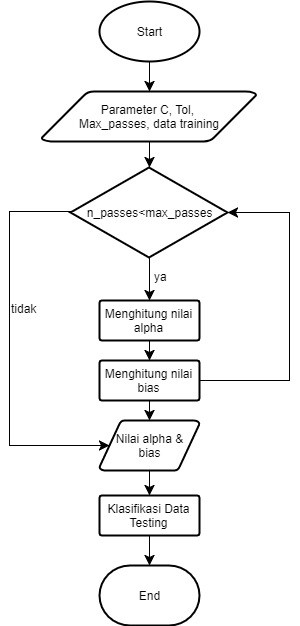
\includegraphics[width=10cm,height=13cm]{images/SVM.jpg}}	
	\captionof{figure}{\textit{Flowchart} Klasifikasi \textit{Support Vector Machine} (SVM) dengan SMO}
\end{minipage}
\end{adjustbox}

\noindent Berikut ini adalah contoh perhitungan klasifikasi teks pada Twitter kelas netral dengan data \textit{training} sebagai berikut:
\begin{table}[H]
	\caption{Data \textit{Training}}
	\centering
	\small
	\begin{adjustbox}{width=1\textwidth}
	\begin{tabular}{|p{2.5cm}|p{1.5cm}|p{1.5cm}|p{1.5cm}|p{1.5cm}|p{1.5cm}|p{1cm}|}
		\hline
		\multirow{2}{*}{\textbf{Dokumen}} & \multicolumn{5}{c|}{\textbf{Kata}}& \multirow{2}{*}{\textbf{Kelas}}\\
		\cline{2-6}
		& \textbf{DPR} & \textbf{Sukses} & \textbf{Semoga} & \textbf{Bagus} & \textbf{Jelek} & \\
		\hline
		D1 & 0.01 & 0.02 & 0.04 & 0.02 & 0.03 & 1 \\
		\hline
		D2 & 0 & 0.003 & 0.02 & 0.01 & 0 & 1 \\
		\hline
		D3 & 0.02 & 0.01 & 0 & 0.01 & 0 & -1 \\
		\hline
		D4 & 0.02 & 0 & 0.03 & 0.04 & 0.05 & -1 \\
		\hline
		D5 & 0 & 0.03 & 0.02 & 0.01 & 0.02 & 1 \\
		\hline
	\end{tabular}
	\end{adjustbox}
\end{table}

\noindent Berikut ini adalah data \textit{testing }yang akan digunakan untuk klasifikasi:

\begin{table}[H]
	\caption{Data \textit{Testing}}
	\centering
	\small
	\begin{adjustbox}{width=1\textwidth}
	\begin{tabular}{|p{2.5cm}|p{1.5cm}|p{1.5cm}|p{1.5cm}|p{1.5cm}|p{1.5cm}|p{1cm}|}
		\hline
		\multirow{2}{*}{\textbf{Dokumen}} & \multicolumn{5}{c|}{\textbf{Kata}}& \multirow{2}{*}{\textbf{Kelas}}\\
		\cline{2-6}
		& \textbf{DPR} & \textbf{Sukses} & \textbf{Semoga} & \textbf{Bagus} & \textbf{Jelek} & \\
		\hline
		T1 & 0.03 & 0 & 0.03 & 0.02 & 0 & ?\\
		\hline
	\end{tabular}
	\end{adjustbox}
\end{table}
Pada tabel 3.30, kelas 1 menunjukan kelas opini positif, sedangkan kelas -1 menunjukkan kelas opini lainnya. Proses dimulai dengan menghitung \textit{kernel} linear dengan menggunakan rumus tabel 2.7. Berikut ini contoh perhitungan nilai \textit{kernel} data \textit{training }pada tabel 3.30:
\begin{table}[H]
	\centering
	\small
	\begin{adjustbox}{width=1\textwidth}
	\begin{tabular}{|p{13.55cm}|}
		\hline
		K(D1,D2) = (0.01*0.01) + (0.02*0.02) + (0.04*0.04) + (0.02*0.02) + 
		(0.03*0.03) = 0.0034\\
		K(D1,D2) = (0.01*0) + (0.02*0.003) + (0.04*0.02) + (0.02*0.01) + (0.03*0) = 0.00106\\
		K(D1,D3) = (0.01*0.02) + (0.02*0.01) + (0.04*0) + (0.02*0.01) + (0.03*0) = 0.0006\\
		K(D1,D4) = (0.01*0.02) + (0.02*0) + (0.04*0.03) + (0.02*0.04) + (0.03*0.05) = 0.0037\\
		K(D1,D5) = (0.01*0) + (0.02*0.03) + (0.04*0.02) + (0.02*0.01) + (0.03*0) = 0.0022 
		\\
		\hline
	\end{tabular}
	\end{adjustbox}
\end{table}
\noindent Berikut ini adalah tabel hasil dari perhitungan \textit{kernel} pada setiap dokumen:
\begin{table}[H]
	\caption{Hasil Perhitungan \textit{Kernel} Linear pada Data \textit{Training}}
	\centering
	\small
	\begin{adjustbox}{width=1\textwidth}
	\begin{tabular}{|p{2cm}|p{2cm}|p{2cm}|p{1.9cm}|p{1.9cm}|p{1.5cm}|}
		\hline
		& \textbf{D1} & \textbf{D2} & \textbf{D3} & \textbf{D4} & \textbf{D5} \\
		\hline
		\textbf{D1} & 0.0034 & 0.00106 & 0.0006 & 0.0037 & 0.0022 \\
		\hline
		\textbf{D2} & 0.00106 & 0.000509 & 0,00013 & 0.001 & 0.00059 \\
		\hline
		\textbf{D3} & 0.0006 & 0.00013 & 0.0006 & 0,0008 & 0.0004 \\
		\hline
		\textbf{D4} & 0.0037 & 0.001 & 0.0008 & 0.0054 & 0.002 \\
		\hline
		\textbf{D5} & 0.0022 & 0.00059 & 0.0004 & 0.002 & 0.0018 \\
		\hline
	\end{tabular}
	\end{adjustbox}
\end{table}
Setelah mendapatkan perhitungan \textit{kernel} linear tahap selanjutnya mencari nilai alpha dan bias dengan algoritme \textit{Simplified} SMO sebagai berikut:
\begin{table}[H]
	\centering
	\small
	\begin{adjustbox}{width=1\textwidth}
	\begin{tabular}{|p{13.55cm}|}
		\hline
		\begin{enumerate}[label={},leftmargin=*,noitemsep]
			\item C=0.05 (Parameter Regularisasi)
			\item Tol=0.0001 (Toleransi Numerik)
			\item maxIter= 2 (maksimal pengulangan yang dilakukan ketika alpha tidak berubah)
			\item $\alpha_{i}$= 0
			\item $\alpha_{i}$(old)= 0
			\item b=0
			\item iter=0
			\item iter $<$ maxIter //kondisi while
			\begin{enumerate}[label={},noitemsep]
				\item jum\_perubahan\_alpha = 0
				\item i = 1//loop sebanyak jumlah dokumen \textit{training}
				\begin{enumerate}[label={},noitemsep]
					\item E$_{i}$ = f(x$_{1}$) - y$_{1}$
					\item = $[$((0 * 1 * 0.0034) + (0 * 1 * 0.000106) + (0 * -1 * 0.0006) + (0 * -1 * 0.0037) 
					+ (0 * 1 * 0.0022)) + 0$]$ - 1
					\item //kondisi if terpenuhi
					\item j = 3 //pilih j random, j != i
					\item E$_{3}$ = f(x$_{3}$) - y$_{3 }$
					\item = $[$((0 * 1 * 0.0006) + (0 * 1 * 0.00013) + (0 * -1 * 0.0006) + (0 * -1 * 0.0008) + (0 * 1 * 0.0004)) + 0$]$ - -1
					\item = 1
					\item $\alpha_{1}$(old) = 0
					\item $\alpha_{3}$(old) = 0
					\item L = max(0,(0-0))=0
					\item H = min(0.05,(0.0.5 + 0 - 0)) = 0.05
					\item //kondisi L!=H //kondisi L!=H terpenuhi
					\item $\eta$ = 2 * 0.06 - 0.16 - 0.09 = (-0.13)
					\item //kondisi eta $<$ 0 terpenuhi
					\item $\alpha_{3}$= 0 - $[$ ((-1 * (-1 - 1))) / (-0.13) $]$ = 15.385
					\item kondisi $\alpha_{3}>$ H terpenuhi
					\item $\alpha_{3}$= 0.05
					\item // kondisi abs($\alpha_{3}$ - $\alpha_{3}$(old)) $>$ 10$^{-5}$ terpenuhi
					\item $\alpha_{ 1 }$= 0 + (1 * -1 * (0 - 0.05)) = 0.05
					\item b$_{1 }$= 0 - (-1) - (1 * (0.05 - 0) * 0.16) - 
					(-1 * (0.05 - 0) * 0.06) = 0.995
					\item b$_{2}$ = 0 - (1) - (1 * (0.05 - 0) * 
					0.06) - (-1 * (0.05 - 0) * 0.09) = -0.9985
					\item b = (0.995 + (-0.9985))/2 = -0.0035
					\item jum\_perubahan\_alpha = 1
								
				\end{enumerate}
				\item //pengulangan dilakukan terus sampai data ke i=5
				\item iter = 0 // kondisi jum\_perubahan\_alpha !=0	
			\end{enumerate}
			\item //pengulangan dilakukan terus sampai kondisi while tidak terpenuhi 	
		\end{enumerate}
		\\
		\hline
	\end{tabular}
	\end{adjustbox}
\end{table}
\noindent Berikut ini adalah nilai alpha dan bias dari perhitungan \textit{simplified} SMO:

\begin{table}[H]
	\caption{Nilai Alpha dan Bias pada perhitungan SMO}
	\centering
	\small
	\begin{adjustbox}{width=1\textwidth}
	\begin{tabular}{|p{1.87cm}|p{1.87cm}|p{1.87cm}|p{1.87cm}|p{1.87cm}|p{2cm}|}
		\hline
		$\alpha_{1}$ & $\alpha_{2}$ & $\alpha_{3}$ & $\alpha_{4}$ & $\alpha_{5}$ & bias\\
		\hline
		0.78 & 0.5 & 0.3 & 0.21 & 0.25 & 0.135 \\
		\hline
	\end{tabular}
	\end{adjustbox}
\end{table}

Setelah mendapatkan nilai alpha dan bias, maka dapat dilakukan klasifikasi teks pada tabel 3.31. Perhitungan klasifikasi \textit{testing} juga dilakukan dengan perhitungan \textit{kernel} linear sebagai berikut:
\begin{table}[H]
	\centering
	\small
	\begin{adjustbox}{width=1\textwidth}	
	\begin{tabular}{|p{13.55cm}|}
		\hline
		K(T1,D1) = (0.03*0.01) + (0*0.02) + (0.03*0.04) + (0.02*0.02) + (0*0.03) = 0.0019\\
		K(T1,D2) = (0.03*0) + (0*0.03) + (0.03*0.02) + (0.02*0.01) + 
		(0*0) = 0.0008\\
		K(T1,D3) = (0.03*0.02) + (0*0.01) + (0.03*0) + (0.02*0.01) 
		+ (0*0) = 0.0008\\
		K(T1,D4) = (0.03*0.02) + (0*0) + (0.03*0.03) + 
		(0.02*0.04) + (0*0.05) = 0.0023\\
		K(T1,D5) = (0.03*0) + (0*0.03) + (0.03*0) 
		+ (0.02*0.03) + (0*0.02) = 0.0008 \\
		\hline
	\end{tabular}
	\end{adjustbox}
\end{table}
\noindent Berikut ini adalah hasil perhitungan \textit{kernel }linear pada data \textit{testing} : 

\begin{table}[H]
	\caption{Hasil Perhitungan \textit{Kernel} Linear pada Data \textit{Testing}}
	\centering
	\small
	\begin{adjustbox}{width=1\textwidth}
	\begin{tabular}{|p{2cm}|p{2cm}|p{2cm}|p{1.9cm}|p{1.9cm}|p{1.5cm}|}
		\hline
		& \textbf{D1} & \textbf{D2} & \textbf{D3} & \textbf{D4} & \textbf{D5} \\
		\hline
		\textbf{T1} & 0.0019 & 0.0008 & 0.0008 & 0.0023 & 0.0008 \\
		\hline
	\end{tabular}
	\end{adjustbox}
\end{table}
\noindent Setelah perhitungan \textit{kernel} linear dilakukan maka dapat dilakukan perhitungan klasifikasi sebagai berikut:
\begin{table}[H]
	\centering
	\small
	\begin{adjustbox}{width=1\textwidth}	
	\begin{tabular}{|p{13.55cm}|}
		\hline
		F(x) = (0.78 * 1 * 0.0019) + (0.5 * 1 * 0.0008) + (0.3 * -1 * 0.0008) + (0.21 * -1 * 0.0023) + (0.25 * 1 * 0.0008) + 0.135 = -1.86 = -1 \\
		\hline
	\end{tabular}
	\end{adjustbox}
\end{table}
Berdasarkan perhitungan di atas, dokumen T1 termasuk dalam kelas 1 yang merupakan kelas bukan netral.
\pagebreak
\subsection{\textit{Class Diagram}}
Berikut ini adalah \textit{design} \textit{class diagram} pada sistem analisis sentimen yang akan dibuat:

	
\begin{adjustbox}{width=1\textwidth}
\noindent\begin{minipage}{\linewidth}
	\framebox[\textwidth]{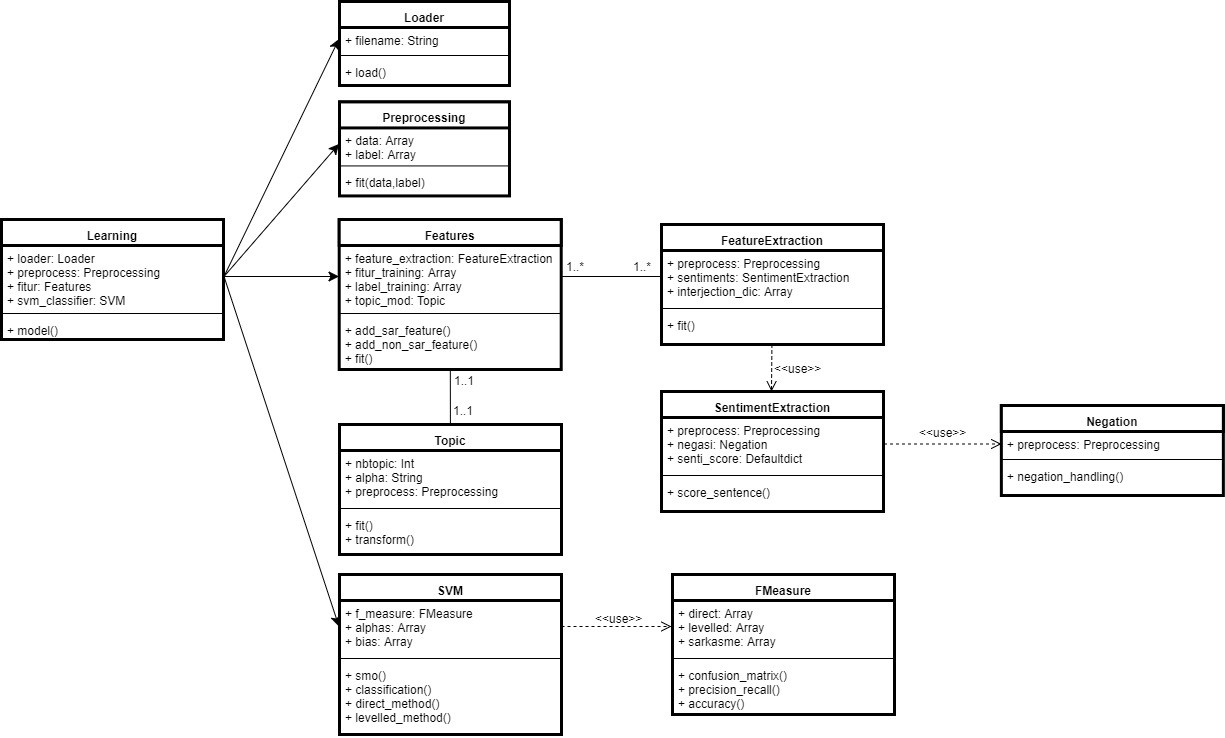
\includegraphics[width=13cm]{images/class_diagram.jpg}}	
	\captionof{figure}{\textit{Class Diagram} Sistem Analisis Sentimen}
\end{minipage}
\end{adjustbox}
\newpage
	\setcounter{page}{1}
	\setlength\LTleft{0pt}            % default: \fill
	\setlength\LTright{0pt}           % default: \fill	
	%-----------------------------------------------------------------------------%
\chapter{IMPLEMENTASI DAN PENGUJIAN}
%-----------------------------------------------------------------------------%

%
\vspace{4.5pt}
Pada bab ini akan menjelaskan tentang pengimplementasian dan pengujian terhadap analisis sentimen yang telah dibangun berdasarkan bab-bab sebelumnya.
\section{Lingkungan Aplikasi}
Dalam aplikasi terbagi menjadi dua bagian, yaitu lingkungan implementasi perangkat keras dan perangkat lunak. Di dalam penelitian ini, perangkat keras yang digunakan adalah:
\begin{enumerate}[leftmargin=*]
	\item Processor Intel Core i3-4150 CPU 3.50GHz Dual Core
	\item RAM 8 GB.
\end{enumerate}

Spesifikasi perangkat lunak yang digunakan untuk pengembangan sistem adalah:
\begin{enumerate}[leftmargin=*]
	\item Sistem Operasi\quad\quad\quad\,: Windows 10 Enterprise 1709 64-bit.
	\item Tool Pengembangan\quad: Eclipse Java EE IDE for Web Developers.
	\item Versi\quad\quad\quad\quad\quad\quad\quad\,: Neon.3 Release (4.6.3).
\end{enumerate}

\section{Daftar \textit{Project}, \textit{Class} dan \textit{Method}}
Pada bagian ini akan dijelaskan mengenai \textit{Project}, \textit{class} dan \textit{method} yang terbentuk pada \textit{prototype} sistem Apertura dengan arsitektur microservice.
\subsection{\textit{Project} Customer}
\textit{Project Customer} berisi susunan \textit{class} pembentuk \textit{webservice customer}. Dalam project ini terdapat 4 buah \textit{package} yang berfungsi untuk memisahkan \textit{class} sesuai dengan fungsinya masing-masing. Ke empat \textit{package} ini yaitu \textit{package} controller yang berisi method-method yang dijalankan pada \textit{web service}, \textit{package} model yang berisi entitas dan tabel, \textit{package} repository yang menghubungkan entitas di \textit{package} model dengan database, dan \textit{package} service yang menginisialisasi \textit{webservice} yang akan terbentuk. Pada bagian ini akan dijelaskan mengenai \textit{class} dan \textit{method} yang digunakan pada pengembangan \textit{ webservice customer}:
\subsubsection{\textit{Package} Controller}
\textit{Package} controller berisi method API yang dapat digunakan untuk berkomunikasi dengan \textit{service} customer. \textit{Class} yang terdapat dalam \textit{package} ini adalah \textit{class} CustomerController dan CustomergroupController yang berisi 5 buah fungsi API. Di bawah ini merupakan daftar \textit{class} untuk \textit{package} controller pada \textit{webservice} customer.
\begin{table}[H]
	\small
	\centering
	\caption{Daftar {\itshape Class} pada {\itshape Package} Controller}
	\begin{adjustbox}{width=1\textwidth}
		\begin{tabular}{| p {3 cm} | p {8 cm} | p {3 cm} |}
			\hline
			{\bfseries Package} & {\bfseries Class} & {\bfseries Jenis Class} \\
			\hline
			\multirow{2}{*}{Controller} & CustomerController & {\itshape Class} \\
			& CustomergroupController & {\itshape Class} \\
			\hline
		\end{tabular}
	\end{adjustbox}
\end{table}
\begin{table}[H]
	\caption{Daftar \textit{Method} pada \textit{Class} CustomerController}
	\centering
	\small
	\begin{adjustbox}{width=1\textwidth}	
		\begin{tabular}{|p{0.4cm}|p{3.2cm}|p{1.4cm}|p{1.7cm}|p{1.55cm}|p{3cm}|}
			\hline
			\multirow{2}{*}{\textbf{No}} & \multirow{2}{*}{\textit{\textbf{Method}}} & \multicolumn{2}{c|}{\textit{\textbf{Input}}} & \multirow{2}{*}{\textit{\textbf{Output}}} & 
			\multirow{2}{*}{\textbf{Keterangan}}\\
			\cline{3-4}
			& & \textbf{Tipe} & \textbf{Variabel} & & \\
			\hline
			1 & addCustomer & void & Customer & Customer, HttpStatus & \textit{Method} ini digunakan untuk membuat \textit{object} customer yang baru melalui \textit{webservice}\\
			\hline
			2 & updateCustomer & void & Customer & HttpStatus & \textit{Method} ini digunakan untuk mengubah attribut dari \textit{object} customer yang baru melalui \textit{webservice}\\
			\hline
			3 & getCustomer & void & id & Customer, HttpStatus & \textit{Method} ini digunakan untuk mengambil satu \textit{object} customer yang baru melalui \textit{webservice}\\
			\hline
		\end{tabular}
	\end{adjustbox}
\end{table}
\begin{table}[H]
	\centering
	\small
	\begin{adjustbox}{width=1\textwidth}	
		\begin{tabular}{|p{0.4cm}|p{2.5cm}|p{1cm}|p{1.1cm}|p{3.4cm}|p{3cm}|}
			\hline
			4 & getAllCustomer & void & - & $<$List$<$Customer$>$$>$, HttpStatus & \textit{Method} ini digunakan untuk mengambil semua \textit{list} \textit{object} customer yang baru melalui \textit{webservice}\\
			\hline
			5 & deleteCustomer & void & id &HttpStatus & \textit{Method} ini digunakan untuk menghapus satu \textit{object} customer yang baru melalui \textit{webservice}\\
			\hline
		\end{tabular}
	\end{adjustbox}
\end{table}
\begin{table}[H]
	\caption{Daftar \textit{Method} pada \textit{Class} CustomergroupController}
	\centering
	\small
	\begin{adjustbox}{width=1\textwidth}	
		\begin{tabular}{|p{0.4cm}|p{3.5cm}|p{1.4cm}|p{1.7cm}|p{1.55cm}|p{3cm}|}
			\hline
			\multirow{2}{*}{\textbf{No}} & \multirow{2}{*}{\textit{\textbf{Method}}} & \multicolumn{2}{c|}{\textit{\textbf{Input}}} & \multirow{2}{*}{\textit{\textbf{Output}}} & 
			\multirow{2}{*}{\textbf{Keterangan}}\\
			\cline{3-4}
			& & \textbf{Tipe} & \textbf{Variabel} & & \\
			\hline
			1 & addCustomerGroup & Customer & customer & customer, HttpStatus & \textit{Method} ini digunakan untuk membuat \textit{object} CustomerGroup yang baru melalui \textit{webservice}\\
			\hline
			2 & updateCustomerGroup & Customer & customer & HttpStatus & \textit{Method} ini digunakan untuk mengubah attribut dari \textit{object} CustomerGroup yang baru melalui \textit{webservice}\\
			\hline
			3 & getCustomerGroup & Customer & customer & customer, HttpStatus & \textit{Method} ini digunakan untuk mengambil satu \textit{object} CustomerGroup yang baru melalui \textit{webservice}\\
			\hline
			4 & getAllCustomerGroup & Customer & customer & customer, HttpStatus & \textit{Method} ini digunakan untuk mengambil semua \textit{list} \textit{object} CustomerGroup yang baru melalui \textit{webservice}\\
			\hline
		\end{tabular}
	\end{adjustbox}
\end{table}
\begin{table}[H]
	\centering
	\small
	\begin{adjustbox}{width=1\textwidth}	
		\begin{tabular}{|p{0.4cm}|p{3.5cm}|p{1.4cm}|p{1.7cm}|p{1.55cm}|p{3cm}|}
			\hline
			5 & deleteCustomerGroup & Customer & customer & customer, HttpStatus & \textit{Method} ini digunakan untuk menghapus satu \textit{object} CustomerGroup yang baru melalui \textit{webservice}\\
			\hline
		\end{tabular}
	\end{adjustbox}
\end{table}
\subsubsection{\textit{Package} Model Customer}
\textit{Package} customer model berisi entitas-entitas penyusun dari \textit{service} customer. Berikut ini merupakan daftar \textit{class} untuk \textit{package} model.
\begin{table}[H]
	\small
	\centering
	\caption{Daftar {\itshape Class} pada {\itshape Package} model}
	\begin{adjustbox}{width=1\textwidth}
		\begin{tabular}{| p {3 cm} | p {8 cm} | p {3 cm} |}
			\hline
			{\bfseries Package} & {\bfseries Class} & {\bfseries Jenis Class} \\
			\hline
			\multirow{13}{*}{Model} & Regency & {\itshape Class} \\
			& AddressType & {\itshape Class} \\
			& Contact & {\itshape Class} \\
			& ContactAddress & {\itshape Class} \\
			& ContactEducation & {\itshape Class} \\
			& Country & {\itshape Class} \\
			& Customer & {\itshape Class} \\
			& Customergroup & {\itshape Class} \\
			& HealthConsumer & {\itshape Class} \\
			& Insurance & {\itshape Class} \\
			& InsuranceBridgeConf & {\itshape Class} \\
			& Profession & {\itshape Class} \\
			& Province & {\itshape Class} \\
			\hline
		\end{tabular}
	\end{adjustbox}
\end{table}
\begin{table}[H]
	\caption{Daftar attribut pada \textit{Class} Customer}
	\centering
	\small
	\begin{adjustbox}{width=1\textwidth}	
		\begin{tabular}{|p{4cm} p{2.1cm} p{3cm} p{3.1cm}|}
			\hline
			\multicolumn{2}{|l}{\textbf{Variabel:}}&\multicolumn{2}{l|}{\textbf{Variabel:}}\\
			boolean&cust\_no&Date&registrationdate\\
			boolean&active&int&idPriceLevel\\
			double&creditlimit&double&disc\\
			Customergroup&customergroup&&\\
			\hline
		\end{tabular}
	\end{adjustbox}
\end{table}

\begin{table}[H]
	\caption{Daftar attribut pada \textit{Class} Customergroup}
	\centering
	\small
	\begin{adjustbox}{width=1\textwidth}	
		\begin{tabular}{|p{4cm} p{2.1cm} p{3cm} p{3.1cm}|}
			\hline
			\multicolumn{2}{|l}{\textbf{Variabel:}}&\multicolumn{2}{l|}{}\\
			long&systemid&&\\
			String&groupname&&\\
			String&memo&&\\
			\hline
		\end{tabular}
	\end{adjustbox}
\end{table}

\begin{table}[H]
	\caption{Daftar attribut pada \textit{Class} Contact}
	\centering
	\small
	\begin{adjustbox}{width=1\textwidth}	
		\begin{tabular}{|p{2cm} p{2.1cm} p{5cm} p{3.1cm}|}
			\hline
			\multicolumn{2}{|l}{\textbf{Variabel:}}&\multicolumn{2}{l|}{\textbf{Variabel:}}\\
			long&systemid&String&initial\\
			String&lastname&int&amountofchildren\\
			int&maritalstatus&List$<$ContactAddress$>$&arrAddress\\
			String&middlename&Collection$<$ContactEducation$>$&arrEdu\\
			Date&birthday&String&notes\\
			String&birthplace&String&officeext\\
			String&bloodtype&String&passportid\\
			double&bodyheight&byte[]&photo\\
			double&bodyweight&String&prefixtitle\\
			String&citizenid&String&sms\\
			String&citizentype&String&suffixtitle\\
			Country&citizenship&Date&sys\_createdate\\
			String&email&String&sys\_creator\\
			String&firstname&Date&sys\_lastupdate\\
			int&gender&String&sys\_lastupdater\\
			String&homephone&String&taxid\\
			String&messaging&String&web\\
			\hline
		\end{tabular}
	\end{adjustbox}
\end{table}
\begin{table}[H]
	\caption{Daftar attribut pada \textit{Class} Contact Address}
	\centering
	\small
	\begin{adjustbox}{width=1\textwidth}	
		\begin{tabular}{|p{4cm} p{2.1cm} p{3cm} p{3.1cm}|}
			\hline
			\multicolumn{2}{|l}{\textbf{Variabel:}}&\multicolumn{2}{l|}{\textbf{Variabel:}}\\
			Long&systemid&String&postcode\\
			AddressType&addresstype&Regency&regency\\
			String&street&boolean&asbillingaddress\\
			String&fax&Date&sys\_createdate\\
			Contact&owner&String&sys\_creator\\
			String&phone&Date&sys\_lastupdate\\
			String&sys\_lastupdater&&\\
			\hline
		\end{tabular}
	\end{adjustbox}
\end{table}
\begin{table}[H]
	\caption{Daftar attribut pada \textit{Class} Address Type}
	\centering
	\small
	\begin{adjustbox}{width=1\textwidth}	
		\begin{tabular}{|p{4cm} p{2.1cm} p{3cm} p{3.1cm}|}
			\hline
			\multicolumn{2}{|l}{\textbf{Variabel:}}&\multicolumn{2}{l|}{\textbf{}}\\
			Integer&systemid&&\\
			String&memo&&\\
			String&typename&&\\
			\hline
		\end{tabular}
	\end{adjustbox}
\end{table}
\begin{table}[H]
	\caption{Daftar attribut pada \textit{Class} Contact Education}
	\centering
	\small
	\begin{adjustbox}{width=1\textwidth}	
		\begin{tabular}{|p{3cm} p{3.1cm} p{3cm} p{3.1cm}|}
			\hline
			\multicolumn{2}{|l}{\textbf{Variabel:}}&\multicolumn{2}{l|}{\textbf{\textbf{Variabel:}}}\\
			Date&finishrolling&Contact&owner\\
			String&gpa&String&sponsors\\
			int&grade&Date&startrolling\\
			String&institutionaladdress&Date&sys\_createdate\\
			String&institutionname&int&sys\_creator\\
			String&major&Date&sys\_lastupdate\\
			String&notes&int&sys\_lastupdater\\
			\hline
		\end{tabular}
	\end{adjustbox}
\end{table}
\begin{table}[H]
	\caption{Daftar attribut pada \textit{Class} Country}
	\centering
	\small
	\begin{adjustbox}{width=1\textwidth}	
		\begin{tabular}{|p{4cm} p{2.1cm} p{3cm} p{3.1cm}|}
			\hline
			\multicolumn{2}{|l}{\textbf{Variabel:}}&\multicolumn{2}{l|}{\textbf{}}\\
			Long&systemid&&\\
			String&name&&\\
			\hline
		\end{tabular}
	\end{adjustbox}
\end{table}
\begin{table}[H]
	\caption{Daftar attribut pada \textit{Class} HealthConsumer}
	\centering
	\small
	\begin{adjustbox}{width=1\textwidth}	
		\begin{tabular}{|p{4cm} p{2.1cm} p{3cm} p{3.1cm}|}
			\hline
			\multicolumn{2}{|l}{\textbf{Variabel:}}&\multicolumn{2}{l|}{\textbf{}}\\
			String&regis\_no&&\\
			Profession&id\_prof&&\\
			Insurance&insurance&&\\
			String&insurance\_type&&\\
			String&insurance\_no&&\\
			String&insurance\_prg&&\\
			\hline
		\end{tabular}
	\end{adjustbox}
\end{table}
\begin{table}[H]
	\caption{Daftar attribut pada \textit{Class} Insurance}
	\centering
	\small
	\begin{adjustbox}{width=1\textwidth}	
		\begin{tabular}{|p{5cm} p{3.1cm} p{2cm} p{2.1cm}|}
			\hline
			\multicolumn{2}{|l}{\textbf{Variabel:}}&\multicolumn{2}{l|}{\textbf{}}\\
			List$<$InsuranceBridgeConf$>$&insuranceBrigdeConfList&&\\
			int&systemid&&\\
			String&insurance&&\\
			String&memo&&\\
			boolean&active&&\\
			boolean&sysbuiltin&&\\
			\hline
		\end{tabular}
	\end{adjustbox}
\end{table}
\begin{table}[H]
	\caption{Daftar attribut pada \textit{Class} InsuranceBridgeConf}
	\centering
	\small
	\begin{adjustbox}{width=1\textwidth}	
		\begin{tabular}{|p{5cm} p{3.1cm} p{2cm} p{2.1cm}|}
			\hline
			\multicolumn{2}{|l}{\textbf{Variabel:}}&\multicolumn{2}{l|}{\textbf{}}\\
			Long&systemid&&\\
			String&field&&\\
			String&def\_val&&\\
			String&memo&&\\
			\hline
		\end{tabular}
	\end{adjustbox}
\end{table}
\begin{table}[H]
	\caption{Daftar attribut pada \textit{Class} Profession}
	\centering
	\small
	\begin{adjustbox}{width=1\textwidth}	
		\begin{tabular}{|p{5cm} p{3.1cm} p{2cm} p{2.1cm}|}
			\hline
			\multicolumn{2}{|l}{\textbf{Variabel:}}&\multicolumn{2}{l|}{\textbf{}}\\
			Integer&systemid&&\\
			String&profname&&\\
			String&memo&&\\
			Calendar&sys\_createdate&&\\
			Calendar&last\_createdate&&\\
			\hline
		\end{tabular}
	\end{adjustbox}
\end{table}
\begin{table}[H]
	\caption{Daftar attribut pada \textit{Class} Province}
	\centering
	\small
	\begin{adjustbox}{width=1\textwidth}	
		\begin{tabular}{|p{5cm} p{3.1cm} p{2cm} p{2.1cm}|}
			\hline
			\multicolumn{2}{|l}{\textbf{Variabel:}}&\multicolumn{2}{l|}{\textbf{}}\\
			Long&systemid&&\\
			Country&countryCode&&\\
			String&name&&\\
			Set$<$Regency$>$&regencySet&&\\
			\hline
		\end{tabular}
	\end{adjustbox}
\end{table}
\begin{table}[H]
	\caption{Daftar attribut pada \textit{Class} Regency}
	\centering
	\small
	\begin{adjustbox}{width=1\textwidth}	
		\begin{tabular}{|p{5cm} p{3.1cm} p{2cm} p{2.1cm}|}
			\hline
			\multicolumn{2}{|l}{\textbf{Variabel:}}&\multicolumn{2}{l|}{\textbf{}}\\
			Long&systemid&&\\
			Province&provId&&\\
			String&name&&\\
			\hline
		\end{tabular}
	\end{adjustbox}
\end{table}
\subsubsection{\textit{Package} Repository}
\textit{Package} repository berisi \textit{class-class} yang menjadi representasi model dari tabel-tabel yang berada pada basis data. Berikut ini merupakan \textit{class-class} yang terdapat pada \textit{package} repository.
\begin{table}[H]
	\small
	\centering
	\caption{Daftar {\itshape Class} pada {\itshape Package} repository}
	\begin{adjustbox}{width=1\textwidth}
		\begin{tabular}{| p {3 cm} | p {8 cm} | p {3 cm} |}
			\hline
			{\bfseries Package} & {\bfseries Class} & {\bfseries Jenis Class} \\
			\hline
			\multirow{2}{*}{repository} & CustomerRepository & {\itshape Interface} \\
			& CustomergroupRepository & {\itshape Interface} \\
			\hline
		\end{tabular}
	\end{adjustbox}
\end{table}
\subsubsection{\textit{Package} Service}
\textit{Package} service berisi \textit{class-class} yang menginisialisasi \textit{web service} customer yang akan terbentuk dan digunakan pada \textit{package} controller. Berikut ini merupakan \textit{class-class} yang terdapat pada \textit{package} service.
\begin{table}[H]
	\small
	\centering
	\caption{Daftar {\itshape Class} pada {\itshape Package} serviec}
	\begin{adjustbox}{width=1\textwidth}
		\begin{tabular}{| p {3 cm} | p {8 cm} | p {3 cm} |}
			\hline
			{\bfseries Package} & {\bfseries Class} & {\bfseries Jenis Class} \\
			\hline
			\multirow{5}{*}{service} & CRUDService & {\itshape Interface} \\
			& CustomergroupService & {\itshape Interface} \\
			& CustomerService & {\itshape Interface} \\
			& DefaultCustomergroupService & {\itshape Class} \\
			& DefaultCustomerService & {\itshape Class} \\
			\hline
		\end{tabular}
	\end{adjustbox}
\end{table}
\subsection{\textit{Project} \textit{Human Resource}}
\textit{Project Human Resource} berisi susunan \textit{class} pembentuk \textit{webservice Human Resource}. Dalam project ini terdapat 4 buah \textit{package} yang berfungsi untuk memisahkan \textit{class} sesuai dengan fungsinya masing-masing. Ke empat \textit{package} ini yaitu \textit{package} controller yang berisi method-method yang dijalankan pada \textit{web service}, \textit{package} model yang berisi entitas dan tabel, \textit{package} repository yang menghubungkan entitas di \textit{package} model dengan database, dan \textit{package} service yang menginisialisasi \textit{webserviec} yang akan terbentuk. Pada bagian ini akan dijelaskan mengenai \textit{class} dan \textit{method} yang digunakan pada pengembangan \textit{ webservice customer}:
\subsubsection{\textit{Package} Controller}
\textit{Package} controller berisi method API yang dapat digunakan untuk berkomunikasi dengan \textit{service} Human Resource. \textit{Class} yang terdapat dalam \textit{package} ini adalah \textit{class} EmployeeController dan JobSpecialityController yang berisi 5 buah fungsi API. Di bawah ini merupakan daftar \textit{class} untuk \textit{package} controller pada \textit{webservice} \textit{Human Resource}.
\begin{table}[H]
	\small
	\centering
	\caption{Daftar {\itshape Class} pada {\itshape Package} Controller}
	\begin{adjustbox}{width=1\textwidth}
		\begin{tabular}{| p {3 cm} | p {8 cm} | p {3 cm} |}
			\hline
			{\bfseries Package} & {\bfseries Class} & {\bfseries Jenis Class} \\
			\hline
			\multirow{2}{*}{Controller} & EmployeeController & {\itshape Class} \\
			& JobspecialityController & {\itshape Class} \\
			\hline
		\end{tabular}
	\end{adjustbox}
\end{table}
\begin{table}[H]
	\caption{Daftar \textit{Method} pada \textit{Class} EmployeeController}
	\centering
	\small
	\begin{adjustbox}{width=1\textwidth}	
		\begin{tabular}{|p{0.4cm}|p{2.5cm}|p{0.9cm}|p{1.5cm}|p{3.4cm}|p{2.5cm}|}
			\hline
			\multirow{2}{*}{\textbf{No}} & \multirow{2}{*}{\textit{\textbf{Method}}} & \multicolumn{2}{c|}{\textit{\textbf{Input}}} & \multirow{2}{*}{\textit{\textbf{Output}}} & 
			\multirow{2}{*}{\textbf{Keterangan}}\\
			\cline{3-4}
			& & \textbf{Tipe} & \textbf{Variabel} & & \\
			\hline
			1 & addEmployee & void & Employee & Employee, HttpStatus & \textit{Method} ini digunakan untuk membuat \textit{object} employee yang baru melalui \textit{webservice}\\
			\hline
			2 & updateEmployee & void & Employee & HttpStatus & \textit{Method} ini digunakan untuk mengubah attribut dari \textit{object} employee yang baru melalui \textit{webservice}\\
			\hline
			3 & getEmployee & void & id & Employee, HttpStatus & \textit{Method} ini digunakan untuk mengambil satu \textit{object} employee yang baru melalui \textit{webservice}\\
			\hline
			4 & getAllEmployees & void & - & $<$List$<$Employee$>$$>$, HttpStatus & \textit{Method} ini digunakan untuk mengambil semua \textit{list} \textit{object} employee yang baru melalui \textit{webservice}\\
			\hline
		\end{tabular}
	\end{adjustbox}
\end{table}
\begin{table}[H]
	\centering
	\small
	\begin{adjustbox}{width=1\textwidth}	
		\begin{tabular}{|p{0.4cm}|p{2.5cm}|p{0.9cm}|p{1.5cm}|p{3.4cm}|p{2.5cm}|}
			\hline
			5 & deleteEmployee & void & id & HttpStatus & \textit{Method} ini digunakan untuk menghapus satu \textit{object} employee yang baru melalui \textit{webservice}\\
			\hline
		\end{tabular}
	\end{adjustbox}
\end{table}
\begin{table}[H]
	\caption{Daftar \textit{Method} pada \textit{Class} JobspecialityController}
	\centering
	\small
	\begin{adjustbox}{width=1\textwidth}	
		\begin{tabular}{|p{0.4cm}|p{3.2cm}|p{0.8cm}|p{1.9cm}|p{2.85cm}|p{2.4cm}|}
			\hline
			\multirow{2}{*}{\textbf{No}} & \multirow{2}{*}{\textit{\textbf{Method}}} & \multicolumn{2}{c|}{\textit{\textbf{Input}}} & \multirow{2}{*}{\textit{\textbf{Output}}} & 
			\multirow{2}{*}{\textbf{Keterangan}}\\
			\cline{3-4}
			& & \textbf{Tipe} & \textbf{Variabel} & & \\
			\hline
			1 & addJobSpeciality & void & Jobspeciality & Jobspeciality, HttpStatus & \textit{Method} ini digunakan untuk membuat \textit{object} Jobspeciality yang baru melalui \textit{webservice}\\
			\hline
			2 & updateJobSpeciality & void & Jobspeciality & HttpStatus & \textit{Method} ini digunakan untuk mengubah attribut dari \textit{object} Jobspeciality yang baru melalui \textit{webservice}\\
			\hline
			3 & getJobSpeciality & void & id & Jobspeciality, HttpStatus & \textit{Method} ini digunakan untuk mengambil satu \textit{object} Jobspeciality yang baru melalui \textit{webservice}\\
			\hline
		\end{tabular}
	\end{adjustbox}
\end{table}
\begin{table}[H]
	\centering
	\small
	\begin{adjustbox}{width=1\textwidth}	
		\begin{tabular}{|p{0.4cm}|p{3.2cm}|p{1.cm}|p{1.7cm}|p{2.75cm}|p{2.5cm}|}
			\hline
			4 & getAllJobsSpeciality & void & - & $<$List
			$<$Jobspeciality$>$$>$, HttpStatus & \textit{Method} ini digunakan untuk mengambil semua \textit{list} \textit{object} Jobspeciality yang baru melalui \textit{webservice}\\
			\hline
			5 & deleteJobSpeciality & void & id & Jobspeciality, HttpStatus & \textit{Method} ini digunakan untuk menghapus satu \textit{object} CustomerGroup yang baru melalui \textit{webservice}\\
			\hline
		\end{tabular}
	\end{adjustbox}
\end{table}
\subsubsection{\textit{Package} Model Human Resource}
\textit{Package} Human Resource model berisi entitas-entitas penyusun dari \textit{service} Human Resource. Berikut ini merupakan daftar \textit{class} untuk \textit{package} model.
\begin{table}[H]
	\small
	\centering
	\caption{Daftar {\itshape Class} pada {\itshape Package} model}
	\begin{adjustbox}{width=1\textwidth}
		\begin{tabular}{| p {3 cm} | p {8 cm} | p {3 cm} |}
			\hline
			{\bfseries Package} & {\bfseries Class} & {\bfseries Jenis Class} \\
			\hline
			\multirow{12}{*}{Model} & Regency & {\itshape Class} \\
			& AddressType & {\itshape Class} \\
			& Contact & {\itshape Class} \\
			& ContactAddress & {\itshape Class} \\
			& ContactEducation & {\itshape Class} \\
			& Country & {\itshape Class} \\
			& Department & {\itshape Class} \\
			& Employee & {\itshape Class} \\
			& Employment & {\itshape Class} \\
			& Jobspeciality & {\itshape Class} \\
			& Province & {\itshape Class} \\
			& RoleInDept & {\itshape Class} \\
			\hline
		\end{tabular}
	\end{adjustbox}
\end{table}
\begin{table}[H]
	\caption{Daftar attribut pada \textit{Class} Employment}
	\centering
	\small
	\begin{adjustbox}{width=1\textwidth}	
		\begin{tabular}{|p{4cm} p{2.1cm} p{3cm} p{3.1cm}|}
			\hline
			\multicolumn{2}{|l}{\textbf{Variabel:}}&\multicolumn{2}{l|}{\textbf{Variabel:}}\\
			Long&systemid&Employee&employee\\
			String&ein&Date&hiredate\\
			BigInteger&basesalary&RoleInDept&roleIndept\\
			Integer&contracttype&String& sourceinstitution\\
			int&sourcetype&Date& createdate\\
			Date&lastupdate&Date& terminatedate\\
			\hline
		\end{tabular}
	\end{adjustbox}
\end{table}
\begin{table}[H]
	\caption{Daftar attribut pada \textit{Class} Employee}
	\centering
	\small
	\begin{adjustbox}{width=1\textwidth}	
		\begin{tabular}{|p{4cm} p{2.1cm} p{3cm} p{3.1cm}|}
			\hline
			\multicolumn{2}{|l}{\textbf{Variabel:}}&\multicolumn{2}{l|}{}\\
			String&m\_ein&&\\
			Jobspeciality&jobspeciality&&\\
			Collection$<$Employment$>$&employmentCollection&&\\
			\hline
		\end{tabular}
	\end{adjustbox}
\end{table}
\begin{table}[H]
	\caption{Daftar attribut pada \textit{Class} Departement}
	\centering
	\small
	\begin{adjustbox}{width=1\textwidth}	
		\begin{tabular}{|p{4cm} p{2.1cm} p{3cm} p{3.1cm}|}
			\hline
			\multicolumn{2}{|l}{\textbf{Variabel:}}&\multicolumn{2}{l|}{\textbf{}}\\
			int&systemid&&\\
			String&deptname&&\\
			String&memo&&\\
			Collection$<$RoleInDept$>$&roles&&\\
			Date&createdate&&\\
			Date&lastupdate&&\\
			\hline
		\end{tabular}
	\end{adjustbox}
\end{table}
\begin{table}[H]
	\caption{Daftar attribut pada \textit{Class} Contact}
	\centering
	\small
	\begin{adjustbox}{width=1\textwidth}	
		\begin{tabular}{|p{2cm} p{2.1cm} p{5cm} p{3.1cm}|}
			\hline
			\multicolumn{2}{|l}{\textbf{Variabel:}}&\multicolumn{2}{l|}{\textbf{Variabel:}}\\
			long&systemid&String&initial\\
			String&lastname&int&amountofchildren\\
			int&maritalstatus&List$<$ContactAddress$>$&arrAddress\\
			String&middlename&Collection$<$ContactEducation$>$&arrEdu\\
			Date&birthday&String&notes\\
			String&birthplace&String&officeext\\
			String&bloodtype&String&passportid\\
			double&bodyheight&byte[]&photo\\
			double&bodyweight&String&prefixtitle\\
			String&citizenid&String&sms\\
			String&citizentype&String&suffixtitle\\
			Country&citizenship&Date&sys\_createdate\\
			String&email&String&sys\_creator\\
			String&firstname&Date&sys\_lastupdate\\
			int&gender&String&sys\_lastupdater\\
			String&homephone&String&taxid\\
			String&messaging&String&web\\
			\hline
		\end{tabular}
	\end{adjustbox}
\end{table}
\begin{table}[H]
	\caption{Daftar attribut pada \textit{Class} ContactAddress}
	\centering
	\small
	\begin{adjustbox}{width=1\textwidth}	
		\begin{tabular}{|p{4cm} p{2.1cm} p{3cm} p{3.1cm}|}
			\hline
			\multicolumn{2}{|l}{\textbf{Variabel:}}&\multicolumn{2}{l|}{\textbf{Variabel:}}\\
			Long&systemid&String&postcode\\
			AddressType&addresstype&Regency&regency\\
			String&street&boolean&asbillingaddress\\
			String&fax&Date&sys\_createdate\\
			Contact&owner&String&sys\_creator\\
			String&phone&Date&sys\_lastupdate\\
			String&sys\_lastupdater&&\\
			\hline
		\end{tabular}
	\end{adjustbox}
\end{table}
\begin{table}[H]
	\caption{Daftar attribut pada \textit{Class} AddressType}
	\centering
	\small
	\begin{adjustbox}{width=1\textwidth}	
		\begin{tabular}{|p{4cm} p{2.1cm} p{3cm} p{3.1cm}|}
			\hline
			\multicolumn{2}{|l}{\textbf{Variabel:}}&\multicolumn{2}{l|}{\textbf{}}\\
			Integer&systemid&&\\
			String&memo&&\\
			String&typename&&\\
			\hline
		\end{tabular}
	\end{adjustbox}
\end{table}
\begin{table}[H]
	\caption{Daftar attribut pada \textit{Class} ContactEducation}
	\centering
	\small
	\begin{adjustbox}{width=1\textwidth}	
		\begin{tabular}{|p{3cm} p{3.1cm} p{3cm} p{3.1cm}|}
			\hline
			\multicolumn{2}{|l}{\textbf{Variabel:}}&\multicolumn{2}{l|}{\textbf{\textbf{Variabel:}}}\\
			Date&finishrolling&Contact&owner\\
			String&gpa&String&sponsors\\
			int&grade&Date&startrolling\\
			String&institutionaladdress&Date&sys\_createdate\\
			String&institutionname&int&sys\_creator\\
			String&major&Date&sys\_lastupdate\\
			String&notes&int&sys\_lastupdater\\
			\hline
		\end{tabular}
	\end{adjustbox}
\end{table}
\begin{table}[H]
	\caption{Daftar attribut pada \textit{Class} Country}
	\centering
	\small
	\begin{adjustbox}{width=1\textwidth}	
		\begin{tabular}{|p{4cm} p{2.1cm} p{3cm} p{3.1cm}|}
			\hline
			\multicolumn{2}{|l}{\textbf{Variabel:}}&\multicolumn{2}{l|}{\textbf{}}\\
			Long&systemid&&\\
			String&name&&\\
			\hline
		\end{tabular}
	\end{adjustbox}
\end{table}
\begin{table}[H]
	\caption{Daftar attribut pada \textit{Class} Jobspeciality}
	\centering
	\small
	\begin{adjustbox}{width=1\textwidth}	
		\begin{tabular}{|p{5cm} p{3.1cm} p{2cm} p{2.1cm}|}
			\hline
			\multicolumn{2}{|l}{\textbf{Variabel:}}&\multicolumn{2}{l|}{\textbf{}}\\
			Long&systemid&&\\
			String&specialityName&&\\
			String&memo&&\\
			\hline
		\end{tabular}
	\end{adjustbox}
\end{table}
\begin{table}[H]
	\caption{Daftar attribut pada \textit{Class} RoleInDept}
	\centering
	\small
	\begin{adjustbox}{width=1\textwidth}	
		\begin{tabular}{|p{5cm} p{3.1cm} p{2cm} p{2.1cm}|}
			\hline
			\multicolumn{2}{|l}{\textbf{Variabel:}}&\multicolumn{2}{l|}{\textbf{}}\\
			int&systemid&&\\
			Department&department&&\\
			String&rolename&&\\
			String&abbreviation&&\\
			RoleInDept&parentRole&&\\
			String&memo&&\\
			\hline
		\end{tabular}
	\end{adjustbox}
\end{table}
\begin{table}[H]
	\caption{Daftar attribut pada \textit{Class} Province}
	\centering
	\small
	\begin{adjustbox}{width=1\textwidth}	
		\begin{tabular}{|p{5cm} p{3.1cm} p{2cm} p{2.1cm}|}
			\hline
			\multicolumn{2}{|l}{\textbf{Variabel:}}&\multicolumn{2}{l|}{\textbf{}}\\
			Long&systemid&&\\
			Country&countryCode&&\\
			String&name&&\\
			Set$<$Regency$>$&regencySet&&\\
			\hline
		\end{tabular}
	\end{adjustbox}
\end{table}
\begin{table}[H]
	\caption{Daftar attribut pada \textit{Class} Regency}
	\centering
	\small
	\begin{adjustbox}{width=1\textwidth}	
		\begin{tabular}{|p{5cm} p{3.1cm} p{2cm} p{2.1cm}|}
			\hline
			\multicolumn{2}{|l}{\textbf{Variabel:}}&\multicolumn{2}{l|}{\textbf{}}\\
			Long&systemid&&\\
			Province&provId&&\\
			String&name&&\\
			\hline
		\end{tabular}
	\end{adjustbox}
\end{table}
\subsubsection{\textit{Package} Repository}
\textit{Package} repository berisi \textit{class-class} yang menjadi representasi model dari tabel-tabel yang berada pada basis data. Berikut ini merupakan \textit{class-class} yang terdapat pada \textit{package} repository.
\begin{table}[H]
	\small
	\centering
	\caption{Daftar {\itshape Class} pada {\itshape Package} repository}
	\begin{adjustbox}{width=1\textwidth}
		\begin{tabular}{| p {3 cm} | p {8 cm} | p {3 cm} |}
			\hline
			{\bfseries Package} & {\bfseries Class} & {\bfseries Jenis Class} \\
			\hline
			\multirow{2}{*}{repository} & EmployeeRepository & {\itshape Interface} \\
			& JobspecialityRepository & {\itshape Interface} \\
			\hline
		\end{tabular}
	\end{adjustbox}
\end{table}
\subsubsection{\textit{Package} Service}
\textit{Package} service berisi \textit{class-class} yang menginisialisasi \textit{web service} human resource yang akan terbentuk dan digunakan pada \textit{package} controller. Berikut ini merupakan \textit{class-class} yang terdapat pada \textit{package} service.
\begin{table}[H]
	\small
	\centering
	\caption{Daftar {\itshape Class} pada {\itshape Package} service}
	\begin{adjustbox}{width=1\textwidth}
		\begin{tabular}{| p {3 cm} | p {8 cm} | p {3 cm} |}
			\hline
			{\bfseries Package} & {\bfseries Class} & {\bfseries Jenis Class} \\
			\hline
			\multirow{5}{*}{service} & CRUDService & {\itshape Interface} \\
			& EmployeeService & {\itshape Interface} \\
			& JobspecialityService & {\itshape Interface} \\
			& DefaultEmployeeService & {\itshape Class} \\
			& DefaultJobspecialityService & {\itshape Class} \\
			\hline
		\end{tabular}
	\end{adjustbox}
\end{table}
\subsection{\textit{Project} \textit{Medical Unit}}
\textit{Project Medical Unit} berisi susunan \textit{class} pembentuk \textit{webservice Medical Unit}. Dalam project ini terdapat 4 buah \textit{package} yang berfungsi untuk memisahkan \textit{class} sesuai dengan fungsinya masing-masing. Ke empat \textit{package} ini yaitu \textit{package} controller yang berisi method-method yang dijalankan pada \textit{web service}, \textit{package} model yang berisi entitas dan tabel, \textit{package} repository yang menghubungkan entitas di \textit{package} model dengan database, dan \textit{package} service yang menginisialisasi \textit{webserviec} yang akan terbentuk. Pada bagian ini akan dijelaskan mengenai \textit{class} dan \textit{method} yang digunakan pada pengembangan \textit{ webservice Unit Medis}:
\subsubsection{\textit{Package} Controller}
\textit{Package} controller berisi method API yang dapat digunakan untuk berkomunikasi dengan \textit{service} Human Resource. \textit{Class} yang terdapat dalam \textit{package} ini adalah \textit{class} UnitmedisController yang berisi 5 buah fungsi API. Di bawah ini merupakan daftar \textit{class} untuk \textit{package} controller pada \textit{webservice} Unit Medis.
\begin{table}[H]
	\small
	\centering
	\caption{Daftar {\itshape Class} pada {\itshape Package} Controller}
	\begin{adjustbox}{width=1\textwidth}
		\begin{tabular}{| p {3 cm} | p {8 cm} | p {3 cm} |}
			\hline
			{\bfseries Package} & {\bfseries Class} & {\bfseries Jenis Class} \\
			\hline
			\multirow{1}{*}{Controller} & UnitmedisController & {\itshape Class} \\
			\hline
		\end{tabular}
	\end{adjustbox}
\end{table}
\begin{table}[H]
	\caption{Daftar \textit{Method} pada \textit{Class} UnitmedisController}
	\centering
	\small
	\begin{adjustbox}{width=1\textwidth}	
		\begin{tabular}{|p{0.4cm}|p{2.8cm}|p{0.9cm}|p{1.8cm}|p{2.8cm}|p{2.5cm}|}
			\hline
			\multirow{2}{*}{\textbf{No}} & \multirow{2}{*}{\textit{\textbf{Method}}} & \multicolumn{2}{c|}{\textit{\textbf{Input}}} & \multirow{2}{*}{\textit{\textbf{Output}}} & 
			\multirow{2}{*}{\textbf{Keterangan}}\\
			\cline{3-4}
			& & \textbf{Tipe} & \textbf{Variabel} & & \\
			\hline
			1 & addMedicalUnit & void & MedicalUnit & MedicalUnit, HttpStatus & \textit{Method} ini digunakan untuk membuat \textit{object} unit medis yang baru melalui \textit{webservice}\\
			\hline
			2 & updateMedicalUnit & void & MedicalUnit & HttpStatus & \textit{Method} ini digunakan untuk mengubah attribut dari \textit{object} unit medis yang baru melalui \textit{webservice}\\
			\hline
			3 & getMedicalUnit & void & id & MedicalUnit, HttpStatus & \textit{Method} ini digunakan untuk mengambil satu \textit{object} unit medis yang baru melalui \textit{webservice}\\
			\hline
			4 & getAllMedicalUnit & void & - & $<$List
			$<$MedicalUnit$>$$>$, HttpStatus & \textit{Method} ini digunakan untuk mengambil semua \textit{list} \textit{object} unit medis yang baru melalui \textit{webservice}\\
			\hline
			5 & deleteMedicalUnit & void & id & HttpStatus & \textit{Method} ini digunakan untuk menghapus satu \textit{object} unit medis yang baru melalui \textit{webservice}\\
			\hline
		\end{tabular}
	\end{adjustbox}
\end{table}
\subsubsection{\textit{Package} Model Medical Unit}
\textit{Package} Medical Unit model berisi entitas-entitas penyusun dari \textit{service} Medical Unit. Berikut ini merupakan daftar \textit{class} untuk \textit{package} model.
\begin{table}[H]
	\small
	\centering
	\caption{Daftar {\itshape Class} pada {\itshape Package} model}
	\begin{adjustbox}{width=1\textwidth}
		\begin{tabular}{| p {3 cm} | p {8 cm} | p {3 cm} |}
			\hline
			{\bfseries Package} & {\bfseries Class} & {\bfseries Jenis Class} \\
			\hline
			\multirow{16}{*}{Model} & MedicalUnit & {\itshape Class} \\
			& WorkingUnit & {\itshape Class} \\
			& WorkingUnitMembership & {\itshape Class} \\
			& WorkingUnitMembershipPK & {\itshape Class} \\
			& WUGroup & {\itshape Class} \\
			& AddressType & {\itshape Class} \\
			& Contact & {\itshape Class} \\
			& ContactAddress & {\itshape Class} \\
			& ContactEducation & {\itshape Class} \\
			& Country & {\itshape Class} \\
			& Department & {\itshape Class} \\
			& Employee & {\itshape Class} \\
			& Employment & {\itshape Class} \\
			& Jobspeciality & {\itshape Class} \\
			& Province & {\itshape Class} \\
			& RoleInDept & {\itshape Class} \\
			& Regency & {\itshape Class} \\
			\hline
		\end{tabular}
	\end{adjustbox}
\end{table}
\begin{table}[H]
	\caption{Daftar attribut pada \textit{Class} WorkingUnit}
	\centering
	\small
	\begin{adjustbox}{width=1\textwidth}	
		\begin{tabular}{|p{4cm} p{2.1cm} p{3cm} p{3.1cm}|}
			\hline
			\multicolumn{2}{|l}{\textbf{Variabel:}}&\multicolumn{2}{l|}{\textbf{Variabel:}}\\
			Long&systemid&&\\
			WUGroup&wugroup&&\\
			String&workunit\_name&&\\
			String&memo&&\\
			Calendar&createdate&&\\
			Calendar&lastupdate&&\\
			\hline
		\end{tabular}
	\end{adjustbox}
\end{table}
\begin{table}[H]
	\caption{Daftar attribut pada \textit{Class} MedicalUnit}
	\centering
	\small
	\begin{adjustbox}{width=1\textwidth}	
		\begin{tabular}{|p{4cm} p{2.1cm} p{3cm} p{3.1cm}|}
			\hline
			\multicolumn{2}{|l}{\textbf{Variabel:}}&\multicolumn{2}{l|}{}\\
			Long&systemid&&\\
			\hline
		\end{tabular}
	\end{adjustbox}
\end{table}
\begin{table}[H]
	\caption{Daftar attribut pada \textit{Class} WorkingUnitMembership}
	\centering
	\small
	\begin{adjustbox}{width=1\textwidth}	
		\begin{tabular}{|p{4cm} p{2.1cm} p{3cm} p{3.1cm}|}
			\hline
			\multicolumn{2}{|l}{\textbf{Variabel:}}&\multicolumn{2}{l|}{}\\
			WorkingUnit&workingunit&&\\
			Employee&employee&&\\
			boolean&workingunitpersonincharge&&\\
			String&description&&\\
			Calendar&sys\_createdate&&\\
			Calendar&syssys\_lastupdate&&\\
			\hline
		\end{tabular}
	\end{adjustbox}
\end{table}
\begin{table}[H]
	\caption{Daftar attribut pada \textit{Class} WUGroup}
	\centering
	\small
	\begin{adjustbox}{width=1\textwidth}	
		\begin{tabular}{|p{4cm} p{2.1cm} p{3cm} p{3.1cm}|}
			\hline
			\multicolumn{2}{|l}{\textbf{Variabel:}}&\multicolumn{2}{l|}{}\\
			Long&systemid&&\\
			String&groupname&&\\
			String&memo&&\\
			\hline
		\end{tabular}
	\end{adjustbox}
\end{table}
\begin{table}[H]
	\caption{Daftar attribut pada \textit{Class} WorkingUnitMembershipPK}
	\centering
	\small
	\begin{adjustbox}{width=1\textwidth}	
		\begin{tabular}{|p{4cm} p{2.1cm} p{3cm} p{3.1cm}|}
			\hline
			\multicolumn{2}{|l}{\textbf{Variabel:}}&\multicolumn{2}{l|}{}\\
			Long&workingunit&&\\
			Long&employee&&\\
			\hline
		\end{tabular}
	\end{adjustbox}
\end{table}
\begin{table}[H]
	\caption{Daftar attribut pada \textit{Class} Employment}
	\centering
	\small
	\begin{adjustbox}{width=1\textwidth}	
		\begin{tabular}{|p{4cm} p{2.1cm} p{3cm} p{3.1cm}|}
			\hline
			\multicolumn{2}{|l}{\textbf{Variabel:}}&\multicolumn{2}{l|}{\textbf{Variabel:}}\\
			Long&systemid&Employee&employee\\
			String&ein&Date&hiredate\\
			BigInteger&basesalary&RoleInDept&roleIndept\\
			Integer&contracttype&String& sourceinstitution\\
			int&sourcetype&Date& createdate\\
			Date&lastupdate&Date& terminatedate\\
			\hline
		\end{tabular}
	\end{adjustbox}
\end{table}
\begin{table}[H]
	\caption{Daftar attribut pada \textit{Class} Employee}
	\centering
	\small
	\begin{adjustbox}{width=1\textwidth}	
		\begin{tabular}{|p{4cm} p{2.1cm} p{3cm} p{3.1cm}|}
			\hline
			\multicolumn{2}{|l}{\textbf{Variabel:}}&\multicolumn{2}{l|}{}\\
			String&m\_ein&&\\
			Jobspeciality&jobspeciality&&\\
			Collection$<$Employment$>$&employmentCollection&&\\
			\hline
		\end{tabular}
	\end{adjustbox}
\end{table}
\begin{table}[H]
	\caption{Daftar attribut pada \textit{Class} Departement}
	\centering
	\small
	\begin{adjustbox}{width=1\textwidth}	
		\begin{tabular}{|p{4cm} p{2.1cm} p{3cm} p{3.1cm}|}
			\hline
			\multicolumn{2}{|l}{\textbf{Variabel:}}&\multicolumn{2}{l|}{\textbf{}}\\
			int&systemid&&\\
			String&deptname&&\\
			String&memo&&\\
			Collection$<$RoleInDept$>$&roles&&\\
			Date&createdate&&\\
			Date&lastupdate&&\\
			\hline
		\end{tabular}
	\end{adjustbox}
\end{table}
\begin{table}[H]
	\caption{Daftar attribut pada \textit{Class} ContactAddress}
	\centering
	\small
	\begin{adjustbox}{width=1\textwidth}	
		\begin{tabular}{|p{4cm} p{2.1cm} p{3cm} p{3.1cm}|}
			\hline
			\multicolumn{2}{|l}{\textbf{Variabel:}}&\multicolumn{2}{l|}{\textbf{Variabel:}}\\
			Long&systemid&String&postcode\\
			AddressType&addresstype&Regency&regency\\
			String&street&boolean&asbillingaddress\\
			String&fax&Date&sys\_createdate\\
			Contact&owner&String&sys\_creator\\
			String&phone&Date&sys\_lastupdate\\
			String&sys\_lastupdater&&\\
			\hline
		\end{tabular}
	\end{adjustbox}
\end{table}
\begin{table}[H]
	\caption{Daftar attribut pada \textit{Class} Contact}
	\centering
	\small
	\begin{adjustbox}{width=1\textwidth}	
		\begin{tabular}{|p{2cm} p{2.1cm} p{5cm} p{3.1cm}|}
			\hline
			\multicolumn{2}{|l}{\textbf{Variabel:}}&\multicolumn{2}{l|}{\textbf{Variabel:}}\\
			long&systemid&String&initial\\
			String&lastname&int&amountofchildren\\
			int&maritalstatus&List$<$ContactAddress$>$&arrAddress\\
			String&middlename&Collection$<$ContactEducation$>$&arrEdu\\
			Date&birthday&String&notes\\
			String&birthplace&String&officeext\\
			String&bloodtype&String&passportid\\
			double&bodyheight&byte[]&photo\\
			double&bodyweight&String&prefixtitle\\
			String&citizenid&String&sms\\
			String&citizentype&String&suffixtitle\\
			Country&citizenship&Date&sys\_createdate\\
			String&email&String&sys\_creator\\
			String&firstname&Date&sys\_lastupdate\\
			int&gender&String&sys\_lastupdater\\
			String&homephone&String&taxid\\
			String&messaging&String&web\\
			\hline
		\end{tabular}
	\end{adjustbox}
\end{table}
\begin{table}[H]
	\caption{Daftar attribut pada \textit{Class} AddressType}
	\centering
	\small
	\begin{adjustbox}{width=1\textwidth}	
		\begin{tabular}{|p{4cm} p{2.1cm} p{3cm} p{3.1cm}|}
			\hline
			\multicolumn{2}{|l}{\textbf{Variabel:}}&\multicolumn{2}{l|}{\textbf{}}\\
			Integer&systemid&&\\
			String&memo&&\\
			String&typename&&\\
			\hline
		\end{tabular}
	\end{adjustbox}
\end{table}
\begin{table}[H]
	\caption{Daftar attribut pada \textit{Class} ContactEducation}
	\centering
	\small
	\begin{adjustbox}{width=1\textwidth}	
		\begin{tabular}{|p{3cm} p{3.1cm} p{3cm} p{3.1cm}|}
			\hline
			\multicolumn{2}{|l}{\textbf{Variabel:}}&\multicolumn{2}{l|}{\textbf{\textbf{Variabel:}}}\\
			Date&finishrolling&Contact&owner\\
			String&gpa&String&sponsors\\
			int&grade&Date&startrolling\\
			String&institutionaladdress&Date&sys\_createdate\\
			String&institutionname&int&sys\_creator\\
			String&major&Date&sys\_lastupdate\\
			String&notes&int&sys\_lastupdater\\
			\hline
		\end{tabular}
	\end{adjustbox}
\end{table}
\begin{table}[H]
	\caption{Daftar attribut pada \textit{Class} Country}
	\centering
	\small
	\begin{adjustbox}{width=1\textwidth}	
		\begin{tabular}{|p{4cm} p{2.1cm} p{3cm} p{3.1cm}|}
			\hline
			\multicolumn{2}{|l}{\textbf{Variabel:}}&\multicolumn{2}{l|}{\textbf{}}\\
			Long&systemid&&\\
			String&name&&\\
			\hline
		\end{tabular}
	\end{adjustbox}
\end{table}
\begin{table}[H]
	\caption{Daftar attribut pada \textit{Class} Jobspeciality}
	\centering
	\small
	\begin{adjustbox}{width=1\textwidth}	
		\begin{tabular}{|p{5cm} p{3.1cm} p{2cm} p{2.1cm}|}
			\hline
			\multicolumn{2}{|l}{\textbf{Variabel:}}&\multicolumn{2}{l|}{\textbf{}}\\
			Long&systemid&&\\
			String&specialityName&&\\
			String&memo&&\\
			\hline
		\end{tabular}
	\end{adjustbox}
\end{table}
\begin{table}[H]
	\caption{Daftar attribut pada \textit{Class} RoleInDept}
	\centering
	\small
	\begin{adjustbox}{width=1\textwidth}	
		\begin{tabular}{|p{5cm} p{3.1cm} p{2cm} p{2.1cm}|}
			\hline
			\multicolumn{2}{|l}{\textbf{Variabel:}}&\multicolumn{2}{l|}{\textbf{}}\\
			int&systemid&&\\
			Department&department&&\\
			String&rolename&&\\
			String&abbreviation&&\\
			RoleInDept&parentRole&&\\
			String&memo&&\\
			\hline
		\end{tabular}
	\end{adjustbox}
\end{table}
\begin{table}[H]
	\caption{Daftar attribut pada \textit{Class} Province}
	\centering
	\small
	\begin{adjustbox}{width=1\textwidth}	
		\begin{tabular}{|p{5cm} p{3.1cm} p{2cm} p{2.1cm}|}
			\hline
			\multicolumn{2}{|l}{\textbf{Variabel:}}&\multicolumn{2}{l|}{\textbf{}}\\
			Long&systemid&&\\
			Country&countryCode&&\\
			String&name&&\\
			Set$<$Regency$>$&regencySet&&\\
			\hline
		\end{tabular}
	\end{adjustbox}
\end{table}
\begin{table}[H]
	\caption{Daftar attribut pada \textit{Class} Regency}
	\centering
	\small
	\begin{adjustbox}{width=1\textwidth}	
		\begin{tabular}{|p{5cm} p{3.1cm} p{2cm} p{2.1cm}|}
			\hline
			\multicolumn{2}{|l}{\textbf{Variabel:}}&\multicolumn{2}{l|}{\textbf{}}\\
			Long&systemid&&\\
			Province&provId&&\\
			String&name&&\\
			\hline
		\end{tabular}
	\end{adjustbox}
\end{table}
\subsubsection{\textit{Package} Repository}
\textit{Package} repository berisi \textit{class-class} yang menjadi representasi model dari tabel-tabel yang berada pada basis data. Berikut ini merupakan \textit{class-class} yang terdapat pada \textit{package} repository.
\begin{table}[H]
	\small
	\centering
	\caption{Daftar {\itshape Class} pada {\itshape Package} repository}
	\begin{adjustbox}{width=1\textwidth}
		\begin{tabular}{| p {3 cm} | p {8 cm} | p {3 cm} |}
			\hline
			{\bfseries Package} & {\bfseries Class} & {\bfseries Jenis Class} \\
			\hline
			\multirow{1}{*}{repository} & UnitmedisRepository & {\itshape Interface} \\
			\hline
		\end{tabular}
	\end{adjustbox}
\end{table}
\subsubsection{\textit{Package} Service}
\textit{Package} service berisi \textit{class-class} yang menginisialisasi \textit{web service} human resource yang akan terbentuk dan digunakan pada \textit{package} controller. Berikut ini merupakan \textit{class-class} yang terdapat pada \textit{package} service.
\begin{table}[H]
	\small
	\centering
	\caption{Daftar {\itshape Class} pada {\itshape Package} service}
	\begin{adjustbox}{width=1\textwidth}
		\begin{tabular}{| p {3 cm} | p {8 cm} | p {3 cm} |}
			\hline
			{\bfseries Package} & {\bfseries Class} & {\bfseries Jenis Class} \\
			\hline
			\multirow{3}{*}{service} & CRUDService & {\itshape Interface} \\
			& UnitmedisService & {\itshape Interface} \\
			& DefaultUnitmedisService & {\itshape Class} \\
			\hline
		\end{tabular}
	\end{adjustbox}
\end{table}
\subsection{\textit{Project} Rawat Jalan}
\textit{Project} Rawat Jalan berisi susunan \textit{class} pembentuk \textit{webservice} Rawat Jalan. Dalam project ini terdapat 4 buah \textit{package} yang berfungsi untuk memisahkan \textit{class} sesuai dengan fungsinya masing-masing. Ke empat \textit{package} ini yaitu \textit{package} controller yang berisi method-method yang dijalankan pada \textit{web service}, \textit{package} model yang berisi entitas dan tabel, \textit{package} repository yang menghubungkan entitas di \textit{package} model dengan database, dan \textit{package} service yang menginisialisasi \textit{webserviec} yang akan terbentuk. Pada bagian ini akan dijelaskan mengenai \textit{class} dan \textit{method} yang digunakan pada pengembangan \textit{webservice} Rawat Jalan:
\subsubsection{\textit{Package} Controller}

\textit{Package} controller berisi method API yang dapat digunakan untuk berkomunikasi dengan \textit{service} Rawat Jalan. \textit{Class} yang terdapat dalam \textit{package} ini adalah \textit{class} OutpatientWUQueueController yang berisi 5 buah fungsi API. Di bawah ini merupakan daftar \textit{class} untuk \textit{package} controller pada \textit{webservice} Rawat Jalan.
\begin{table}[H]
	\small
	\centering
	\caption{Daftar {\itshape Class} pada {\itshape Package} Controller}
	\begin{adjustbox}{width=1\textwidth}
		\begin{tabular}{| p {3 cm} | p {8 cm} | p {3 cm} |}
			\hline
			{\bfseries Package} & {\bfseries Class} & {\bfseries Jenis Class} \\
			\hline
			\multirow{1}{*}{Controller} & OutpatientWUQueueController & {\itshape Class} \\
			\hline
		\end{tabular}
	\end{adjustbox}
\end{table}
\begin{table}[H]
	\caption{Daftar \textit{Method} pada \textit{Class} OutpatientWUQueueController}
	\centering
	\small
	\begin{adjustbox}{width=1\textwidth}	
		\begin{tabular}{|p{0.4cm}|p{2.8cm}|p{0.9cm}|p{1.8cm}|p{2.8cm}|p{2.5cm}|}
			\hline
			\multirow{2}{*}{\textbf{No}} & \multirow{2}{*}{\textit{\textbf{Method}}} & \multicolumn{2}{c|}{\textit{\textbf{Input}}} & \multirow{2}{*}{\textit{\textbf{Output}}} & 
			\multirow{2}{*}{\textbf{Keterangan}}\\
			\cline{3-4}
			& & \textbf{Tipe} & \textbf{Variabel} & & \\
			\hline
			1 & addOutpatient
			Queue & void & Outpatient
			WUQueue & Outpatient
			WUQueue, HttpStatus & \textit{Method} ini digunakan untuk membuat \textit{object} rawat jalan yang baru melalui \textit{webservice}\\
			\hline
			2 & updateOutpatient
			Queue & void & Outpatient
			WUQueue & HttpStatus & \textit{Method} ini digunakan untuk mengubah attribut dari \textit{object} rawat jalan yang baru melalui \textit{webservice}\\
			\hline
			3 & getOutpatient
			Queue & void & id & Outpatient
			WUQueue, HttpStatus & \textit{Method} ini digunakan untuk mengambil satu \textit{object} rawat jalan yang baru melalui \textit{webservice}\\
			\hline
			4 & getAllOut
			patientQueue & void & - & $<$List
			$<$OutpatientWU
			Queue$>$$>$, HttpStatus & \textit{Method} ini digunakan untuk mengambil semua \textit{list} \textit{object} rawat jalan yang baru melalui \textit{webservice}\\
			\hline
			5 & deleteOutpatient
			Queue & void & id & HttpStatus & \textit{Method} ini digunakan untuk menghapus satu \textit{object} rawat jalan yang baru melalui \textit{webservice}\\
			\hline
		\end{tabular}
	\end{adjustbox}
\end{table}
\subsubsection{\textit{Package} Model Rawat Jalan}
\textit{Package} Rawat Jalan model berisi entitas-entitas penyusun dari \textit{service} Rawat Jalan. Berikut ini merupakan daftar \textit{class} untuk \textit{package} model.
\begin{table}[H]
	\small
	\centering
	\caption{Daftar {\itshape Class} pada {\itshape Package} model}
	\begin{adjustbox}{width=1\textwidth}
		\begin{tabular}{| p {3 cm} | p {8 cm} | p {3 cm} |}
			\hline
			{\bfseries Package} & {\bfseries Class} & {\bfseries Jenis Class} \\
			\hline
			\multirow{26}{*}{Model} & OutpatientWUQueue & {\itshape Class} \\
			& OutpatientWUQueueHistory & {\itshape Class} \\
			& OutpatientWUQueuePK & {\itshape Class} \\
			& WorkingUnit & {\itshape Class} \\
			& WorkingUnitMembership & {\itshape Class} \\
			& WorkingUnitMembershipPK & {\itshape Class} \\
			& WUGroup & {\itshape Class} \\
			& AddressType & {\itshape Class} \\
			& Contact & {\itshape Class} \\
			& ContactAddress & {\itshape Class} \\
			& ContactEducation & {\itshape Class} \\
			& Customer & {\itshape Class} \\
			& Customergroup & {\itshape Class} \\
			& HealthConsumer & {\itshape Class} \\
			& Insurance & {\itshape Class} \\
			& InsuranceBridgeConf & {\itshape Class} \\
			& Profession & {\itshape Class} \\
			& Country & {\itshape Class} \\
			& Department & {\itshape Class} \\
			& Employee & {\itshape Class} \\
			& Employment & {\itshape Class} \\
			& Jobspeciality & {\itshape Class} \\
			& Province & {\itshape Class} \\
			& RoleInDept & {\itshape Class} \\
			& Regency & {\itshape Class} \\
			& MedicalUnit & {\itshape Class} \\
			\hline
		\end{tabular}
	\end{adjustbox}
\end{table}
\begin{table}[H]
	\caption{Daftar attribut pada \textit{Class} OutpatientWUQueue}
	\centering
	\small
	\begin{adjustbox}{width=1\textwidth}	
		\begin{tabular}{|p{4.5cm} p{2.1cm} p{2.5cm} p{3.1cm}|}
			\hline
			\multicolumn{2}{|l}{\textbf{Variabel:}}&\multicolumn{2}{l|}{\textbf{\textbf{Variabel:}}}\\
			OutpatientWUQueue&hc&Calendar&syscreatetime\\
			MedicalUnit&medunit&Calendar&syslastupdate\\
			String&regis\_no&Insurance&insurance\\
			Date&registertimee&String&insuranceno\\
			Date&finishtime&String&insurancetype\\
			int&priority&String&via\\
			String&memo&String&rujukan\_tipe\\
			String&rujukan\_doc\_no&String&rujukan\_nama\_asal\\
			OutpatientWUQueueHistory&history&String&insuranceprg\\
			\hline
		\end{tabular}
	\end{adjustbox}
\end{table}
\begin{table}[H]
	\caption{Daftar attribut pada \textit{Class} outpatienthistory}
	\centering
	\small
	\begin{adjustbox}{width=1\textwidth}	
		\begin{tabular}{|p{3.5cm} p{3.1cm} p{2.5cm} p{3.1cm}|}
			\hline
			\multicolumn{2}{|l}{\textbf{Variabel:}}&\multicolumn{2}{l|}{\textbf{\textbf{Variabel:}}}\\
			OutpatientWUQueue&hc&Calendar&syscreatetime\\
			MedicalUnit&medunit&Calendar&syslastupdate\\
			String&regis\_no&Insurance&insurance\\
			Date&registertimee&String&insuranceno\\
			Date&finishtime&String&insurancetype\\
			int&priority&String&via\\
			String&memo&String&rujukan\_tipe\\
			String&rujukan\_nama\_asal&String&rujukan\_doc\_no\\
			String&insuranceprg&&\\
			\hline
		\end{tabular}
	\end{adjustbox}
\end{table}
\begin{table}[H]
	\caption{Daftar attribut pada \textit{Class} OutpatientWUQueuePK}
	\centering
	\small
	\begin{adjustbox}{width=1\textwidth}	
		\begin{tabular}{|p{4cm} p{2.1cm} p{3cm} p{3.1cm}|}
			\hline
			\multicolumn{2}{|l}{\textbf{Variabel:}}&\multicolumn{2}{l|}{\textbf{}}\\
			long&hc&&\\
			long&medunit&&\\
			\hline
		\end{tabular}
	\end{adjustbox}
\end{table}
\begin{table}[H]
	\caption{Daftar attribut pada \textit{Class} HealthConsumer}
	\centering
	\small
	\begin{adjustbox}{width=1\textwidth}	
		\begin{tabular}{|p{4cm} p{2.1cm} p{3cm} p{3.1cm}|}
			\hline
			\multicolumn{2}{|l}{\textbf{Variabel:}}&\multicolumn{2}{l|}{\textbf{}}\\
			String&regis\_no&&\\
			Profession&id\_prof&&\\
			Insurance&insurance&&\\
			String&insurance\_type&&\\
			String&insurance\_no&&\\
			String&insurance\_prg&&\\
			\hline
		\end{tabular}
	\end{adjustbox}
\end{table}
\begin{table}[H]
	\caption{Daftar attribut pada \textit{Class} Insurance}
	\centering
	\small
	\begin{adjustbox}{width=1\textwidth}	
		\begin{tabular}{|p{5cm} p{3.1cm} p{2cm} p{2.1cm}|}
			\hline
			\multicolumn{2}{|l}{\textbf{Variabel:}}&\multicolumn{2}{l|}{\textbf{}}\\
			List$<$InsuranceBridgeConf$>$&insuranceBrigdeConfList&&\\
			int&systemid&&\\
			String&insurance&&\\
			String&memo&&\\
			boolean&active&&\\
			boolean&sysbuiltin&&\\
			\hline
		\end{tabular}
	\end{adjustbox}
\end{table}
\begin{table}[H]
	\caption{Daftar attribut pada \textit{Class} InsuranceBridgeConf}
	\centering
	\small
	\begin{adjustbox}{width=1\textwidth}	
		\begin{tabular}{|p{5cm} p{3.1cm} p{2cm} p{2.1cm}|}
			\hline
			\multicolumn{2}{|l}{\textbf{Variabel:}}&\multicolumn{2}{l|}{\textbf{}}\\
			Long&systemid&&\\
			String&field&&\\
			String&def\_val&&\\
			String&memo&&\\
			\hline
		\end{tabular}
	\end{adjustbox}
\end{table}
\begin{table}[H]
	\caption{Daftar attribut pada \textit{Class} Profession}
	\centering
	\small
	\begin{adjustbox}{width=1\textwidth}	
		\begin{tabular}{|p{5cm} p{3.1cm} p{2cm} p{2.1cm}|}
			\hline
			\multicolumn{2}{|l}{\textbf{Variabel:}}&\multicolumn{2}{l|}{\textbf{}}\\
			Integer&systemid&&\\
			String&profname&&\\
			String&memo&&\\
			Calendar&sys\_createdate&&\\
			Calendar&last\_createdate&&\\
			\hline
		\end{tabular}
	\end{adjustbox}
\end{table}
\begin{table}[H]
	\caption{Daftar attribut pada \textit{Class} Customer}
	\centering
	\small
	\begin{adjustbox}{width=1\textwidth}	
		\begin{tabular}{|p{4cm} p{2.1cm} p{3cm} p{3.1cm}|}
			\hline
			\multicolumn{2}{|l}{\textbf{Variabel:}}&\multicolumn{2}{l|}{\textbf{Variabel:}}\\
			boolean&cust\_no&Date&registrationdate\\
			boolean&active&int&idPriceLevel\\
			double&creditlimit&double&disc\\
			Customergroup&customergroup&&\\
			\hline
		\end{tabular}
	\end{adjustbox}
\end{table}

\begin{table}[H]
	\caption{Daftar attribut pada \textit{Class} Customergroup}
	\centering
	\small
	\begin{adjustbox}{width=1\textwidth}	
		\begin{tabular}{|p{4cm} p{2.1cm} p{3cm} p{3.1cm}|}
			\hline
			\multicolumn{2}{|l}{\textbf{Variabel:}}&\multicolumn{2}{l|}{}\\
			long&systemid&&\\
			String&groupname&&\\
			String&memo&&\\
			\hline
		\end{tabular}
	\end{adjustbox}
\end{table}
\begin{table}[H]
	\caption{Daftar attribut pada \textit{Class} WorkingUnit}
	\centering
	\small
	\begin{adjustbox}{width=1\textwidth}	
		\begin{tabular}{|p{4cm} p{2.1cm} p{3cm} p{3.1cm}|}
			\hline
			\multicolumn{2}{|l}{\textbf{Variabel:}}&\multicolumn{2}{l|}{\textbf{}}\\
			Long&systemid&&\\
			WUGroup&wugroup&&\\
			String&workunit\_name&&\\
			String&memo&&\\
			Calendar&createdate&&\\
			Calendar&lastupdate&&\\
			\hline
		\end{tabular}
	\end{adjustbox}
\end{table}
\begin{table}[H]
	\caption{Daftar attribut pada \textit{Class} MedicalUnit}
	\centering
	\small
	\begin{adjustbox}{width=1\textwidth}	
		\begin{tabular}{|p{4cm} p{2.1cm} p{3cm} p{3.1cm}|}
			\hline
			\multicolumn{2}{|l}{\textbf{Variabel:}}&\multicolumn{2}{l|}{}\\
			Long&systemid&&\\
			\hline
		\end{tabular}
	\end{adjustbox}
\end{table}
\begin{table}[H]
	\caption{Daftar attribut pada \textit{Class} WorkingUnitMembership}
	\centering
	\small
	\begin{adjustbox}{width=1\textwidth}	
		\begin{tabular}{|p{4cm} p{2.1cm} p{3cm} p{3.1cm}|}
			\hline
			\multicolumn{2}{|l}{\textbf{Variabel:}}&\multicolumn{2}{l|}{}\\
			WorkingUnit&workingunit&&\\
			Employee&employee&&\\
			boolean&workingunitpersonincharge&&\\
			String&description&&\\
			Calendar&sys\_createdate&&\\
			Calendar&syssys\_lastupdate&&\\
			\hline
		\end{tabular}
	\end{adjustbox}
\end{table}
\begin{table}[H]
	\caption{Daftar attribut pada \textit{Class} WUGroup}
	\centering
	\small
	\begin{adjustbox}{width=1\textwidth}	
		\begin{tabular}{|p{4cm} p{2.1cm} p{3cm} p{3.1cm}|}
			\hline
			\multicolumn{2}{|l}{\textbf{Variabel:}}&\multicolumn{2}{l|}{}\\
			Long&systemid&&\\
			String&groupname&&\\
			String&memo&&\\
			\hline
		\end{tabular}
	\end{adjustbox}
\end{table}
\begin{table}[H]
	\caption{Daftar attribut pada \textit{Class} WorkingUnitMembershipPK}
	\centering
	\small
	\begin{adjustbox}{width=1\textwidth}	
		\begin{tabular}{|p{4cm} p{2.1cm} p{3cm} p{3.1cm}|}
			\hline
			\multicolumn{2}{|l}{\textbf{Variabel:}}&\multicolumn{2}{l|}{}\\
			Long&workingunit&&\\
			Long&employee&&\\
			\hline
		\end{tabular}
	\end{adjustbox}
\end{table}
\begin{table}[H]
	\caption{Daftar attribut pada \textit{Class} Employment}
	\centering
	\small
	\begin{adjustbox}{width=1\textwidth}	
		\begin{tabular}{|p{4cm} p{2.1cm} p{3cm} p{3.1cm}|}
			\hline
			\multicolumn{2}{|l}{\textbf{Variabel:}}&\multicolumn{2}{l|}{\textbf{Variabel:}}\\
			Long&systemid&Employee&employee\\
			String&ein&Date&hiredate\\
			BigInteger&basesalary&RoleInDept&roleIndept\\
			Integer&contracttype&String& sourceinstitution\\
			int&sourcetype&Date& createdate\\
			Date&lastupdate&Date& terminatedate\\
			\hline
		\end{tabular}
	\end{adjustbox}
\end{table}
\begin{table}[H]
	\caption{Daftar attribut pada \textit{Class} Employee}
	\centering
	\small
	\begin{adjustbox}{width=1\textwidth}	
		\begin{tabular}{|p{4cm} p{2.1cm} p{3cm} p{3.1cm}|}
			\hline
			\multicolumn{2}{|l}{\textbf{Variabel:}}&\multicolumn{2}{l|}{}\\
			String&m\_ein&&\\
			Jobspeciality&jobspeciality&&\\
			Collection$<$Employment$>$&employmentCollection&&\\
			\hline
		\end{tabular}
	\end{adjustbox}
\end{table}
\begin{table}[H]
	\caption{Daftar attribut pada \textit{Class} Departement}
	\centering
	\small
	\begin{adjustbox}{width=1\textwidth}	
		\begin{tabular}{|p{4cm} p{2.1cm} p{3cm} p{3.1cm}|}
			\hline
			\multicolumn{2}{|l}{\textbf{Variabel:}}&\multicolumn{2}{l|}{\textbf{}}\\
			int&systemid&&\\
			String&deptname&&\\
			String&memo&&\\
			Collection$<$RoleInDept$>$&roles&&\\
			Date&createdate&&\\
			Date&lastupdate&&\\
			\hline
		\end{tabular}
	\end{adjustbox}
\end{table}
\begin{table}[H]
	\caption{Daftar attribut pada \textit{Class} ContactAddress}
	\centering
	\small
	\begin{adjustbox}{width=1\textwidth}	
		\begin{tabular}{|p{4cm} p{2.1cm} p{3cm} p{3.1cm}|}
			\hline
			\multicolumn{2}{|l}{\textbf{Variabel:}}&\multicolumn{2}{l|}{\textbf{Variabel:}}\\
			Long&systemid&String&postcode\\
			AddressType&addresstype&Regency&regency\\
			String&street&boolean&asbillingaddress\\
			String&fax&Date&sys\_createdate\\
			Contact&owner&String&sys\_creator\\
			String&phone&Date&sys\_lastupdate\\
			String&sys\_lastupdater&&\\
			\hline
		\end{tabular}
	\end{adjustbox}
\end{table}
\begin{table}[H]
	\caption{Daftar attribut pada \textit{Class} Contact}
	\centering
	\small
	\begin{adjustbox}{width=1\textwidth}	
		\begin{tabular}{|p{2cm} p{2.1cm} p{5cm} p{3.1cm}|}
			\hline
			\multicolumn{2}{|l}{\textbf{Variabel:}}&\multicolumn{2}{l|}{\textbf{Variabel:}}\\
			long&systemid&String&initial\\
			String&lastname&int&amountofchildren\\
			int&maritalstatus&List$<$ContactAddress$>$&arrAddress\\
			String&middlename&Collection$<$ContactEducation$>$&arrEdu\\
			Date&birthday&String&notes\\
			String&birthplace&String&officeext\\
			String&bloodtype&String&passportid\\
			double&bodyheight&byte[]&photo\\
			double&bodyweight&String&prefixtitle\\
			String&citizenid&String&sms\\
			String&citizentype&String&suffixtitle\\
			Country&citizenship&Date&sys\_createdate\\
			String&email&String&sys\_creator\\
			String&firstname&Date&sys\_lastupdate\\
			int&gender&String&sys\_lastupdater\\
			String&homephone&String&taxid\\
			String&messaging&String&web\\
			\hline
		\end{tabular}
	\end{adjustbox}
\end{table}
\begin{table}[H]
	\caption{Daftar attribut pada \textit{Class} AddressType}
	\centering
	\small
	\begin{adjustbox}{width=1\textwidth}	
		\begin{tabular}{|p{4cm} p{2.1cm} p{3cm} p{3.1cm}|}
			\hline
			\multicolumn{2}{|l}{\textbf{Variabel:}}&\multicolumn{2}{l|}{\textbf{}}\\
			Integer&systemid&&\\
			String&memo&&\\
			String&typename&&\\
			\hline
		\end{tabular}
	\end{adjustbox}
\end{table}
\begin{table}[H]
	\caption{Daftar attribut pada \textit{Class} ContactEducation}
	\centering
	\small
	\begin{adjustbox}{width=1\textwidth}	
		\begin{tabular}{|p{3cm} p{3.1cm} p{3cm} p{3.1cm}|}
			\hline
			\multicolumn{2}{|l}{\textbf{Variabel:}}&\multicolumn{2}{l|}{\textbf{\textbf{Variabel:}}}\\
			Date&finishrolling&Contact&owner\\
			String&gpa&String&sponsors\\
			int&grade&Date&startrolling\\
			String&institutionaladdress&Date&sys\_createdate\\
			String&institutionname&int&sys\_creator\\
			String&major&Date&sys\_lastupdate\\
			String&notes&int&sys\_lastupdater\\
			\hline
		\end{tabular}
	\end{adjustbox}
\end{table}
\begin{table}[H]
	\caption{Daftar attribut pada \textit{Class} Country}
	\centering
	\small
	\begin{adjustbox}{width=1\textwidth}	
		\begin{tabular}{|p{4cm} p{2.1cm} p{3cm} p{3.1cm}|}
			\hline
			\multicolumn{2}{|l}{\textbf{Variabel:}}&\multicolumn{2}{l|}{\textbf{}}\\
			Long&systemid&&\\
			String&name&&\\
			\hline
		\end{tabular}
	\end{adjustbox}
\end{table}
\begin{table}[H]
	\caption{Daftar attribut pada \textit{Class} Jobspeciality}
	\centering
	\small
	\begin{adjustbox}{width=1\textwidth}	
		\begin{tabular}{|p{5cm} p{3.1cm} p{2cm} p{2.1cm}|}
			\hline
			\multicolumn{2}{|l}{\textbf{Variabel:}}&\multicolumn{2}{l|}{\textbf{}}\\
			Long&systemid&&\\
			String&specialityName&&\\
			String&memo&&\\
			\hline
		\end{tabular}
	\end{adjustbox}
\end{table}
\begin{table}[H]
	\caption{Daftar attribut pada \textit{Class} RoleInDept}
	\centering
	\small
	\begin{adjustbox}{width=1\textwidth}	
		\begin{tabular}{|p{5cm} p{3.1cm} p{2cm} p{2.1cm}|}
			\hline
			\multicolumn{2}{|l}{\textbf{Variabel:}}&\multicolumn{2}{l|}{\textbf{}}\\
			int&systemid&&\\
			Department&department&&\\
			String&rolename&&\\
			String&abbreviation&&\\
			RoleInDept&parentRole&&\\
			String&memo&&\\
			\hline
		\end{tabular}
	\end{adjustbox}
\end{table}
\begin{table}[H]
	\caption{Daftar attribut pada \textit{Class} Province}
	\centering
	\small
	\begin{adjustbox}{width=1\textwidth}	
		\begin{tabular}{|p{5cm} p{3.1cm} p{2cm} p{2.1cm}|}
			\hline
			\multicolumn{2}{|l}{\textbf{Variabel:}}&\multicolumn{2}{l|}{\textbf{}}\\
			Long&systemid&&\\
			Country&countryCode&&\\
			String&name&&\\
			Set$<$Regency$>$&regencySet&&\\
			\hline
		\end{tabular}
	\end{adjustbox}
\end{table}
\begin{table}[H]
	\caption{Daftar attribut pada \textit{Class} Regency}
	\centering
	\small
	\begin{adjustbox}{width=1\textwidth}	
		\begin{tabular}{|p{5cm} p{3.1cm} p{2cm} p{2.1cm}|}
			\hline
			\multicolumn{2}{|l}{\textbf{Variabel:}}&\multicolumn{2}{l|}{\textbf{}}\\
			Long&systemid&&\\
			Province&provId&&\\
			String&name&&\\
			\hline
		\end{tabular}
	\end{adjustbox}
\end{table}
\subsubsection{\textit{Package} Repository}
\textit{Package} repository berisi \textit{class-class} yang menjadi representasi model dari tabel-tabel yang berada pada basis data. Berikut ini merupakan \textit{class-class} yang terdapat pada \textit{package} repository.
\begin{table}[H]
	\small
	\centering
	\caption{Daftar {\itshape Class} pada {\itshape Package} repository}
	\begin{adjustbox}{width=1\textwidth}
		\begin{tabular}{| p {3 cm} | p {8 cm} | p {3 cm} |}
			\hline
			{\bfseries Package} & {\bfseries Class} & {\bfseries Jenis Class} \\
			\hline
			\multirow{1}{*}{repository} & OutpatientWUQueueRepository & {\itshape Interface} \\
			\hline
		\end{tabular}
	\end{adjustbox}
\end{table}
\subsubsection{\textit{Package} Service}
\textit{Package} service berisi \textit{class-class} yang menginisialisasi \textit{web service} human resource yang akan terbentuk dan digunakan pada \textit{package} controller. Berikut ini merupakan \textit{class-class} yang terdapat pada \textit{package} service.
\begin{table}[H]
	\small
	\centering
	\caption{Daftar {\itshape Class} pada {\itshape Package} service}
	\begin{adjustbox}{width=1\textwidth}
		\begin{tabular}{| p {3 cm} | p {8 cm} | p {3 cm} |}
			\hline
			{\bfseries Package} & {\bfseries Class} & {\bfseries Jenis Class} \\
			\hline
			\multirow{3}{*}{service} & CRUDService & {\itshape Interface} \\
			& OutpatientWUQueueService & {\itshape Interface} \\
			& DefaultOutpatientWUQueueService & {\itshape Class} \\
			\hline
		\end{tabular}
	\end{adjustbox}
\end{table}
\section{Perbandingan Model Arsitektur Microservice dan Monolitik}
Pada bagian ini akan dilakukan pengujian dalam bentuk perbandingan terhadap kedua jenis model arsitektur. Perbandingan dilakukan dengan memberikan analisa dari cara sistem bekerja pada kedua jenis arsitektur untuk setiap parameter uji yang terdiri dari : tingkat performa, availabilitas, skalabilitas, dan reliabilitas dari sistem.

Setiap analisis perbandingan arsitektur didasarkan oleh kasus nyata yang benar terjadi pada perangkat lunak Apertura dalam kurun waktu 1 tahun terakhir. Hal ini dimaksudkan untuk melihat apakah arsitektur microservice benar dapat menjadi solusi untuk setiap tantangan yang dihadapi perangkat lunak Apertura yang mengimplementasi desain arsitektur monolitik.
Berikut hasil analisa perbandingan dari kedua arsitektur :
\begin{enumerate}[leftmargin=*]
	\item Tingkat Reliabilitas. Sebuah sistem yang \textit{reliable} harus dapat memberikan kinerja yang dapat dipercaya oleh \textit{clients} dan ekosistem tempat sistem itu berada. Bagi seorang anggota pengembang, tingkat reliabilitas juga berpengaruh dalam tahap \textit{development} dan \textit{deployment}, tim pengembang harus memastikan sistem yang mereka buat dapat \textit{reliable} bukan hanya dari sudut pandang mereka saja, namun juga untuk anggota pengembang lain
	\begin{table}[H]
		\small
		\begin{adjustbox}{width=1\textwidth}
			\begin{tabular}{| p {2 cm} | p {10 cm} |}
				\hline
				Arsitektur & Perbandingan Tingkat Reliabilitas\\
				\hline
				\textbf{Monolitik} & Salah satu tantangan yang dihadapi pada arsitektur Apertura adalah banyaknya fitur yang terhambat untuk dikembangkan. Salah satu fitur yang ingin dikembangkan adalah fitur "Laporan Insiden Rumah Sakit", fitur ini berfungsi untuk mencatat insiden yang terjadi di RS, seperti kecelakaan, komplain dari pasien, kejadian tidak terduga di rumah sakit serta dampaknya. Masalah yang menjadi alasan untuk pengembangan fitur ini adalah banyaknya \textit{code} yang masih belum seragam pada sistem. Akibatnya, \textit{developer} Apertura menjadi ragu untuk mengembangkan fitur atau \textit{code} buatannya mereka sendiri karena dikhawatirkan dapat menyebabkan keseluruhan sistem \textit{broken} dan berujung pada banyaknya \textit{bug} pada sistem.
				
				Hal ini apabila ditelaah lebih lanjut dikarenakan model \textit{development} yang terikat dengan keterbatasan desain monolitik itu sendiri yang disebabkan tingginya level \textit{coupling}. Kelemahan tingkat \textit{coupling} yang tinggi menjadikan perubahan yang terjadi pada sebuah modul berdampak pada modul lainnya, menjadikan tim pengembang tidak dapat bekerja secara mandiri dan fokus pada modulnya masing-masing.\\
				\hline
				\textbf{Microservice} & Tantangan yang dihadapi oleh perangkat Apertura dapat dapat diperbaiki dengan menerapkan konsep microservice. Dengan memisahkan \textit{table database} untuk fitur "Laporan Insiden Rumah Sakit" dari modul lain, \textit{developer} tidak perlu takut membuat sistem \textit{broken}, karena proses pengembangan terenkapsulasi dari modul lain. Hal ini ditunjang kelebihan arsitektur microservice yang menjadikan sistem lebih mandiri dan \textit{less coupled} mendukung lingkungan \textit{development} untuk menjadi lebih mandiri dan fokus pada modul masing-masing, sehingga perubahan yang tim pengembang lakukan dalam suatu modul tidak akan bertentangan dengan modul lain.
				
				\textit{Drawback} : 
				\begin{enumerate}[leftmargin=*]
					\item Tidak 100\% menghilangkan tingkat \textit{coupling}. Perubahan pada objek atau alamat dari\textit{web API} masih perlu diketahui oleh tim pengembang lain.
				\end{enumerate}\\
				\hline
			\end{tabular}
		\end{adjustbox}
	\end{table}
	\newpage
	\item Perbandingan Performa. Kemampuan sistem untuk menangani masalah yang diberikan dan seberapa efisien sistem menggunakan sumber daya yang tersedia (seperti \textit{hardware} dan komponen infrastruktur lainnya) serta penanganan dan pemrosesan tugas yang tepat.
	\begin{table}[H]
		\small
		\begin{adjustbox}{width=1\textwidth}
			\begin{tabular}{| p {2 cm} | p {10 cm} |}
				\hline
				Arsitektur & Perbandingan Performa\\
				\hline
				\textbf{Monolitik} & Arsitektur monolitik memberikan performa yang lebih baik dan cepat memberikan \textit{response} balasan ketika berhubungan dengan \textit{database}, hal ini karena pengambilan data dan \textit{join} yang mudah dilakukan antar tabel dalam 1 database.
				
				\textit{Drawback} :
				\begin{enumerate}[leftmargin=*]
					\item Cenderung terjadi \textit{bottleneck effect} pada sistem ketika menangani \textit{request} yang banyak. Contoh kasus yang dapat dijadikan contoh adalah ketika sistem dipaksa untuk menangani \textit{request} yang banyak dalam satu waktu bersamaan. Karena pada arsitektur monolitik hanya terdapat 1 buah \textit{handler} untuk menangani \textit{request}. Seperti pada modul rawat jalan, dimana banyak \textit{user} melakukan pendaftaran di saat bersamaan pada beberapa \textit{counter} pendaftaran. Akibatnya \textit{user} yang ingin meminta jadwal unit medis bertugas harus mengantri bersamaan dengan \textit{request} pendaftaran rawat jalan, yang mengakibatkan respon dari sistem lebih lama.
				\end{enumerate}\\
				\hline
				\textbf{Microservice} & Performa sistem akan menurun karena mengharuskan \textit{join} data dengan service lain. Solusi untuk dapat menangani kelemahan ini adalah melakukan join pada level \textit{programming}, dimana data hasil \textit{response} di load pada sistem, kemudian melakukan \textit{in-memory join}.
				
				Namun masalah \textit{bottleneck effect} dapat lebih teratasi pada arsitektur microservice, dikarenakan antrian \textit{request} dapat diurai sesuai dengan modul yang akan memberikan \textit{response} balasan, menjadikan sistem lebih \textit{responsive} terhadap \textit{request} yang banyak. Pada contoh kasus, \textit{user} yang ingin meminta jadwal unit medis bertugas tidak perlu antri dengan \textit{user} yang melakukan \textit{request} pendaftaran rawat jalan dikarena \textit{handler} modul rawat jalan dengan unit medis sudah \textit{independent}, menjadikan kinerja sistem lebih cepat.\\
				\hline
			\end{tabular}
		\end{adjustbox}
	\end{table}
	\newpage
	\item Tingkat Availabilitas. Availabilitas menjadi salah satu parameter yang penting untuk mengukur seberapa baik sistem bekerja. Apabila sebuah sistem memiliki tingkat \textit{downtime} yang rendah, maka fitur-fitur dalam sistem tersebut dapat bekerja dengan optimal.
	\begin{table}[H]
		\small
		\begin{adjustbox}{width=1\textwidth}
			\begin{tabular}{| p {2 cm} | p {10 cm} |}
				\hline
				Arsitektur & Perbandingan Tingkat Availabilitas\\
				\hline
				\textbf{Monolitik} & Untuk membandingkan seberapa besar tingkat availabilitas dari sistem Apertura, maka akan diangkat sebuah skenario masalah yang pernah terjadi pada sistem, yaitu ketika sistem diharuskan untuk sementara waktu berada pada \textit{status down} untuk melakukan \textit{maintenance} atau perbahan pada \textit{database}. Dalam penelitian ini, modul-modul yang tercipta untuk jasa rawat jalan rumah sakit ada 4 modul, yaitu modul \textit{customer, human resources, medical unit,} dan modul \textit{outpatient}. Total fitur yang ada dari semua modul tersebut berjumlah 13 fitur.
				
				(\textit{Customer}: Menampilkan data pasien dan mencari pasien. \textit{Human Resources}: Menampilkan data dokter, edit data dokter, dan mencari dokter. \textit{Medical Unit}: Menampilkan data \textit{medical unit}, menambah \textit{medical unit} baru, menghapus \textit{medical unit}, dan mencari \textit{medical unit}. \textit{Outpatient}: Menampilkan, menambah, menghapus, dan mencari data rawat jalan.)
				
				Dalam arsitektur monolitik, \textit{status down} yang terjadi mengharuskan sistem untuk tidak berfungsi sementara, yang dimana berarti semua fitur tidak akan berfungsi seluruhnya dikarenakan modul-modul bergantung pada 1 buah database dalam sebuah \textit{server} terpusat.
				\\
				\hline
				\textbf{Microservice} & Pada model arsitektur microservice, \textit{status down} yang terjadi tidak akan menyebabkan keseluruhan fitur menjadi lumpuh. Misalnya apabila mengharuskan terjadi \textit{down} pada modul rawat jalan, maka fitur menampilkan, menambah, menghapus, dan mencari data rawat jalan akan tidak dapat berfungsi, namun 9 fitur yang lain seperti melihat unit medis bertugas, melihat data dokter dan data pasien akan tetap berjalan dengan normal. Menjadikan sistem lebih \textit{high availability}.
				
				\textit{Drawback} : 
				\begin{enumerate}[leftmargin=*]
					\item Cost yang lebih besar dikarenakan kebutuhan menyiapkan \textit{server} tambahan untuk setiap service yang di\textit{deploy}.
					\item Dibutuhkan usaha yang lebih besar untuk mengawasi banyak \textit{server}.
				\end{enumerate}\\
				\hline
			\end{tabular}
		\end{adjustbox}
	\end{table}
	\newpage
	\item Skalabilitas. Kemampuan sistem untuk beradaptasi terhadap perubahan yang terjadi. Sebuah sistem yang gagal untuk beradaptasi terhadap perubahan akan meningkatkan tingkat latensi, tingkat availabilitas yang rendah, bahkan sampai pada meningkatkan resiko \textit{crash}. Sistem yang skalabilitasnya tinggi akan menjadi sistem yang siap bertumbuh dan menjadi lebih besar.
	\begin{table}[H]
		\small
		\begin{adjustbox}{width=1\textwidth}
			\begin{tabular}{| p {2 cm} | p {10 cm} |}
				\hline
				Arsitektur & Perbandingan Skalabilitas Sistem\\
				\hline
				\textbf{Monolitik} & Skenario yang dapat diangkat untuk melihat seberapa besar tingkat skalabilitas dari perangkat lunak Apertura adalah dengan menganalisa bagaimana sistem akan berubah saat sistem menjadi besar. Dalam arsitektur monolitik, sistem dapat direplikasi menjadi 2 buah monolitik yang identik. Kegunaan dari replikasi ini adalah mengantisipasi apabila sistem pertama tidak dapat atau mulai turun performanya ketika sistem bertambah besar, maka sistem replika siap membantu. Sebagai contoh sistem pertama mulai sibuk dengan pendaftaran antrian rawat jalan yang baru, maka sistem replika dapat membantu untuk menangani permintaan melihat unit medis bertugas atau melihat data dokter. Namun kelemahan dari metode ini pada monolitik adalah replikasi membutuhkan biaya yang besar dikarenakan sistem monolitik yang begitu besar dan tidak terpisahkan.\\
				\hline
				\textbf{Microservice} & Sifat microservice yang 'moduler' baik sebagai solusi untuk mendukung sistem ketika sistem butuh beradaptasi. Service yang cenderung sibuk dapat direplikasi dan diakses menggunakan alamat API yang berbeda dan disimpan pada databasenya masing-masing. Misalnya untuk kasus rawat jalan, pendaftaran dapat menggunakan 2 service rawat jalan yang berbeda halaman. Lalu data dari 2 service tersebut di \textit{load} dan ditampilan pada halaman rawat jalan kemudian \textit{sorting} berdasarkan waktu pendaftaran. Kelebihan yang dirasakan adalah replikasi tidak mengharuskan dilakukan pada keseluruhan sistem, melainkan hanya modul yang lebih padat.
				
				\textit{Drawback} : 
				\begin{enumerate}[leftmargin=*]
					\item Melakukan \textit{deployment} pada microservice lebih kompleks karena memungkinkan konfigurasi yang berbeda untuk setiap service.
					\item Membutuhkan integrasi lanjutan agar dapat bersinergi dengan service lain. Misalnya harus memberi tahu service lain apabila terjadi perubahan alamat IP (internet protocol) pada \textit{web API}.
				\end{enumerate}\\
				\hline
			\end{tabular}
		\end{adjustbox}
	\end{table}
\end{enumerate}
\newpage
	\setcounter{page}{1}
	%-----------------------------------------------------------------------------%
\chapter{PENUTUP}
%-----------------------------------------------------------------------------%

%
\vspace{4.5pt}
Bab ini berisi kesimpulan dan saran dari implementasi dan perbandingan performa arsitektur microservice dengan monolitik.
\section{Kesimpulan}
Kesimpulan dari pembuatan sistem analisis dan 
pengujian-pengujian yang telah dilakukan adalah sebagai berikut:
\begin{enumerate}
	\item Untuk dapat melakukan migrasi dari aplikasi monolitik menjadi microservice dibutuhkan perencanaan yang matang, dimulai dari analisis proses bisnis aplikasi, menentukan service yang akan terbentuk, memilih teknologi yang akan digunakan, memilih cara berkomunikasi, dan memilih metode deployment yang tepat.
	\item Desain arsitektur microservice dapat menjadi solusi dalam menyelesaikan tantangan yang menjadi kendala dalam arsitektur monolitik dan cocok untuk diterapkan pada perangkat lunak Apertura.
	\item Arsitektur microservice lebih cocok untuk diimplementasi  pada sistem yang memiliki landasan yang kuat dan siap untuk berkembang menjadi aplikasi yang besar.
	\item Dibutuhkan tools automasi yang lebih banyak untuk diterapkan pada aplikasi berbasis microservice agar mencapai hasil performa yang maksimal.
\end{enumerate}
\section{Saran}
Saran dari penulis untuk pengembangan yang dilakukan untuk arsitektur microservic adalah:
\begin{enumerate}
	\item Lebih banyak eksplorasi dan menggunakan tools yang dapat menunjang kemudahan deployment dari arsitektur microservice.
	\item Menggunakan \textit{framework} untuk penunjang integritas data.
\end{enumerate}
\newpage
	
	
	
	\pagenumbering{roman}
	\setcounter{page}{\thesavepage}
	\fancypagestyle{plain}{%
		\renewcommand{\headrulewidth}{0pt}%
		\fancyhf{}%
		\fancyfoot[c]{\thepage}%
	}
	\cfoot{\thepage}
	\rfoot{}
	
	% Merubah Nama Bibliografi ke Daftar Pustaka
	\renewcommand{\bibname}{DAFTAR PUSTAKA}
	\phantomsection
	\addcontentsline{toc}{chapter}{DAFTAR PUSTAKA}
	% Daftar Pustaka
	
\begin{thebibliography}{7}

\bibitem{1}
{Ramadhani, R. A. A., Indriani, F., \& Nugrahadi, D. T. \emph{Comparison of Naive Bayes Smoothing Methods for Twitter Sentiment Analysis. Comparison of Naive Bayes Smoothing Methods for Twitter Sentiment Analysis.}}
\bibitem{2}
{Tsytsarau, M., \& Palpanas, T. (2012). Survey on mining subjective data on the web. \emph{Data Mining and Knowledge Discovery,} 24(3), 478-514}
\bibitem{3}
{Ptáček, T., Habernal, I., \& Hong, J. (2014). Sarcasm detection on czech and english Twitter. In \emph{Proceedings of COLING 2014, the 25th International Conference on Computational Linguistics: Technical Papers} (pp. 213-223).}
\bibitem{4}
{Peng, C. C., Lakis, M., \& Pan, J. W. Detecting Sarcasm in Text.}
\bibitem{5}
{Lunando, E., \& Purwarianti, A. (2013, September). \emph{Indonesian social media sentiment analysis with sarcasm detection.} In \emph{Advanced Computer Science and Information Sistems (ICACSIS), 2013 International Conference on} (pp. 195-198). IEEE.}
\bibitem{6}
{Java, A., Song, X., Finin, T., \& Tseng, B. (2007, August). Why we Twitter: understanding microblogging usage and communities. In \emph{Proceedings of the 9th WebKDD and 1st SNA-KDD 2007 workshop on Web mining and social network analysis}(pp. 56-65). ACM.}

\bibitem{7}
{Karamizadeh, S., Abdullah, S. M., Halimi, M., Shayan, J., \& javad Rajabi, M. (2014, September). Advantage and drawback of \emph{Support Vector Machine} functionality. In \emph{Computer, Communications, and Control Technology (I4CT), 2014 International Conference on} (pp. 63-65). IEEE.}

\bibitem{8}
{Malouf, R. (2002, August). A comparison of algorithms for \emph{Maximum Entropy} parameter estimation. In \emph{proceedings of the 6th conference on Natural language learning-Volume 20 }(pp. 1-7). Association for Computational Linguistics.}

\bibitem{9}
{Chowdhury, G. G. (2003). Natural language processing. \emph{Annual review of information science and technology,} 37(1), 51-89.}

\bibitem{10}
{Liu, B. (2012). Sentiment analysis and opinion mining. \emph{Synthesis lectures on human language technologies, }5(1), 1-167.}

\bibitem{11}
{Baştanlar, Y., \& Özuysal, M. (2014). Introduction to machine learning. \emph{miRNomics: MicroRNA Biology and Computational Analysis,} 105-128.}

\bibitem{12}
{Adriani, M., Asian, J., Nazief, B., Tahaghoghi, S. M., \& Williams, H. E. (2007). Stemming Indonesian: A confix-stripping approach. \emph{ACM Transactions on Asian Language Information Processing (TALIP), }6(4), 1-33.}

\bibitem{13}
{Wicaksono, A. F., \& Purwarianti, A. (2010, August). HMM based part-of-speech tagger for Bahasa Indonesia. In \emph{Fourth International MALINDO Workshop, Jakarta.}}

\bibitem{14}
{Blei, D. M., Ng, A. Y., \& Jordan, M. I. (2003). Latent dirichlet allocation. \emph{Journal of machine Learning research, }3(Jan), 993-1022.}

\bibitem{15}
{Shabtai, A., Moskovitch, R., Elovici, Y., \& Glezer, C. (2009). Detection of malicious code by applying machine learning classifiers on static features: A state-of-the-art survey. \emph{information security technical report,} 14(1), 16-29. }

\bibitem{16}
{Berwick, R. (2003). An Idiot’s guide to Support Vector Machines (SVMs). \emph{Retrieved on October, }21, 2011.}

\bibitem{17}
{Wang, Z., \& Xue, X. (2014). Multi-class \emph{Support Vector Machine}. In \emph{Support Vector Machines Applications }(pp. 23-48). Springer International Publishing.}

\bibitem{18}
{CS 229, Autumn 2009 “The Simplified SMO Algorithm”.}

\bibitem{19}
{Kwak, H., Lee, C., Park, H., \& Moon, S. (2010, April). What is Twitter, a social network or a news media?. In \emph{Proceedings of the 19th international conference on World wide web }(pp. 591-600). ACM.}

\bibitem{20}
{Shamay-Tsoory, S. G., Tomer, R., \& Aharon-Peretz, J. (2005). The neuroanatomical basis of understanding sarcasm and its relationship to social cognition. \emph{Neuropsychology,} 19(3), 288.}
\end{thebibliography}

	
	%
	% Lampiran 
	%
	
	\setcounter{originalpagenumber}{\number\value{page}}%
	\setcounter{page}{0}
	\pagenumbering{arabic}
	
	\onehalfspacing
	\begin{appendix}
		%
% @author  Andreas Febrian
% @version 1.00 
% 
% Hanya sebuah pembatas bertuliskan LAMPIRAN ditengah halaman. 
% 

\begin{titlepage}
	\centering 
	\vspace*{6cm}
	\noindent \Huge{LAMPIRAN}
\end{titlepage}
	\end{appendix}
	
	\pagenumbering{arabic}% 
	\setcounter{page}{\number\value{originalpagenumber}}
	\clearpage
	\phantomsection \addcontentsline{toc}{chapter}{LAMPIRAN}
	
\end{document}